% Capitolul 5: Modele VAR bayesiene, modele factoriale și nowcasting
% Analiza avansată a seriilor de timp și previziune -- Programul de master Statistică aplicată și data science, anul I, semestrul 2, Academia de Studii Economice din București
% GENERAT de latex/build_chapter5.py -- modificați generatorul, nu acest fișier.

\newcommand{\coursename}{Analiza avansată a seriilor de timp și previziune}
\def\atslang{ro}
% Preambul comun ATS -- Analiza avansată a seriilor de timp și previziune / Advanced Time Series Analysis and Forecasting
% (Beamer, 16:9). Același design ca MFM, SFM și TSA (copiat din TSA, 5 octombrie 2026). Înainte de % Preambul comun ATS -- Analiza avansată a seriilor de timp și previziune / Advanced Time Series Analysis and Forecasting
% (Beamer, 16:9). Același design ca MFM, SFM și TSA (copiat din TSA, 5 octombrie 2026). Înainte de % Preambul comun ATS -- Analiza avansată a seriilor de timp și previziune / Advanced Time Series Analysis and Forecasting
% (Beamer, 16:9). Același design ca MFM, SFM și TSA (copiat din TSA, 5 octombrie 2026). Înainte de \input{../../latex/preamble} se definește
%   \newcommand{\coursename}{Advanced Time Series Analysis and Forecasting}          (EN)
%   \newcommand{\coursename}{Analiza avansată a seriilor de timp și previziune}       (RO)  și  \def\atslang{ro}
% Fișierele .tex se află în EN/Courses, EN/Seminars, RO/Cursuri, RO/Seminarii (două niveluri sub rădăcină).
% Deck-urile sînt generate de latex/build_chapterN.py / build_seminarN.py (vezi latex/ats_build.py).

\documentclass[9pt, aspectratio=169, t]{beamer}
\providecommand{\coursename}{Advanced Time Series Analysis and Forecasting}

% Ensure content fits on slides
\setbeamersize{text margin left=8mm, text margin right=8mm}
% Smaller institute font (title page)
\setbeamerfont{institute}{size=\footnotesize}

%=============================================================================
% THEME AND STYLE CONFIGURATION
%=============================================================================
\usetheme{default}
% Using default theme for clean header/footer control

% Color Palette (matching Redispatch PDF)
\definecolor{MainBlue}{RGB}{26, 58, 110}
\definecolor{AccentBlue}{RGB}{26, 58, 110}
\definecolor{IDAred}{RGB}{205, 0, 0}
\definecolor{DarkGray}{RGB}{51, 51, 51}
\definecolor{MediumGray}{RGB}{128, 128, 128}
\definecolor{LightGray}{RGB}{248, 248, 248}
\definecolor{VeryLightGray}{RGB}{235, 235, 235}
\definecolor{KeynoteGray}{RGB}{218, 218, 218}
\definecolor{SectionGray}{RGB}{120, 120, 120}
\definecolor{FooterGray}{RGB}{100, 100, 100}
\definecolor{Crimson}{RGB}{220, 53, 69}
\definecolor{Forest}{RGB}{46, 125, 50}
\definecolor{Amber}{RGB}{181, 133, 63}
\definecolor{Orange}{RGB}{230, 126, 34}
\definecolor{Purple}{RGB}{142, 68, 173}

% Gradient background (exact Keynote 315° gradient: white to RGB 218,218,218)
\setbeamertemplate{background}{%
    \begin{tikzpicture}[remember picture, overlay]
        \shade[shading=axis, shading angle=315,
        top color=white, bottom color=KeynoteGray]
        (current page.south west) rectangle (current page.north east);
    \end{tikzpicture}%
}
% Fallback solid color for compatibility
\setbeamercolor{background canvas}{bg=}

\setbeamercolor{palette primary}{bg=MainBlue, fg=white}
\setbeamercolor{palette secondary}{bg=MainBlue!85, fg=white}
\setbeamercolor{palette tertiary}{bg=MainBlue!70, fg=white}
\setbeamercolor{structure}{fg=MainBlue}
\setbeamercolor{title}{fg=IDAred}
\setbeamercolor{frametitle}{fg=IDAred, bg=}
\setbeamercolor{block title}{bg=MainBlue, fg=white}
\setbeamercolor{block body}{bg=VeryLightGray, fg=DarkGray}
\setbeamercolor{block title alerted}{bg=Crimson, fg=white}
\setbeamercolor{block body alerted}{bg=Crimson!8, fg=DarkGray}
\setbeamercolor{block title example}{bg=Forest, fg=white}
\setbeamercolor{block body example}{bg=Forest!8, fg=DarkGray}
\setbeamercolor{item}{fg=MainBlue}

% Footer colors (override Madrid theme blue)
\setbeamercolor{author in head/foot}{fg=FooterGray, bg=}
\setbeamercolor{title in head/foot}{fg=FooterGray, bg=}
\setbeamercolor{date in head/foot}{fg=FooterGray, bg=}
\setbeamercolor{section in head/foot}{fg=FooterGray, bg=}
\setbeamercolor{subsection in head/foot}{fg=FooterGray, bg=}

% Bullet styles (apply everywhere including blocks)
\setbeamertemplate{itemize item}{\color{MainBlue}$\boxdot$}
\setbeamertemplate{itemize subitem}{\color{MainBlue}$\blacktriangleright$}
\setbeamertemplate{itemize subsubitem}{\color{MainBlue}\tiny$\bullet$}
\setbeamertemplate{itemize/enumerate body begin}{\normalsize}
\setbeamertemplate{itemize/enumerate subbody begin}{\normalsize}

% Item spacing - compact style
\setlength{\leftmargini}{10pt}       % Level 1: minimal indent
\setlength{\leftmarginii}{10pt}      % Level 2: minimal additional indent
% Compact list spacing (zero extra space before/after lists in blocks)
\makeatletter
\def\@listi{\leftmargin\leftmargini \topsep 0pt \parsep 0pt \itemsep 0pt}
\def\@listii{\leftmargin\leftmarginii \topsep 0pt \parsep 0pt \itemsep 0pt}
\makeatother

\setbeamertemplate{navigation symbols}{}

%=============================================================================
% CUSTOM HEADLINE
%=============================================================================
\setbeamertemplate{headline}{%
    \vskip10pt%
    \hbox to \paperwidth{%
        \hskip0.5cm%
        {\small\color{FooterGray}\renewcommand{\hyperlink}[2]{##2}\insertsectionhead}%
        \hfill%
        \textcolor{FooterGray}{\small\insertframenumber}%
        \hskip0.5cm%
    }%
    \vskip4pt%
    {\color{FooterGray}\hrule height 0.4pt}%
}

%=============================================================================
% CUSTOM FOOTER
%=============================================================================
\usepackage{fontawesome5}

\setbeamertemplate{footline}{%
    {\color{FooterGray}\hrule height 0.4pt}%
    \vskip4pt%
    \hbox to \paperwidth{%
        \hskip0.5cm%
        \textcolor{FooterGray}{\small\coursename}%
        \hfill%
        \raisebox{-0.1em}{%
            \begin{tikzpicture}[x=0.08em, y=0.08em, line width=0.4pt]
                \draw[FooterGray] (0,3) -- (1,4) -- (2,3.5) -- (3,5) -- (4,4) -- (5,6) -- (6,5.5) -- (7,4) -- (8,5) -- (9,7) -- (10,6) -- (11,5) -- (12,6.5) -- (13,8) -- (14,7) -- (15,6) -- (16,7.5) -- (17,9) -- (18,8) -- (19,7) -- (20,8.5) -- (21,10) -- (22,9) -- (23,8) -- (24,9.5);
            \end{tikzpicture}%
        }%
        \hskip0.5cm%
    }%
    \vskip6pt%
}

%=============================================================================
% PACKAGES
%=============================================================================
\usepackage[utf8]{inputenc}
\DeclareUnicodeCharacter{03B1}{\ensuremath{\alpha}}
\usepackage[T1]{fontenc}
\usepackage{amsmath, amssymb, amsthm}
\usepackage{mathtools}
\usepackage{bm}
\usepackage{tikz}
\usetikzlibrary{arrows.meta, positioning, shapes, calc, decorations.pathreplacing, shadings}
\usepackage{booktabs}
\usepackage{multirow}
\usepackage{array}
\usepackage{graphicx}
\usepackage{animate}
\usepackage{hyperref}
\usepackage{colortbl}
\usepackage{listings}
\lstset{language=Python, basicstyle=\ttfamily\scriptsize, keywordstyle=\color{MainBlue}\bfseries,
  commentstyle=\color{Forest}, stringstyle=\color{Crimson}, breaklines=true,
  frame=none, backgroundcolor=\color{VeryLightGray}, xleftmargin=2mm}
\hypersetup{colorlinks=true, linkcolor=MainBlue, urlcolor=MainBlue}
\graphicspath{{../../logos/}{../../charts/}{../../photos/}}
\usepackage{xcolor}
\hfuzz=2pt  % Suppress tiny overfull warnings (<2pt)
\vfuzz=2pt  % Suppress tiny vertical overfull warnings (<2pt)

%=============================================================================
% QUANTLET COMMANDS
%   \quantlet{<displayed name>}{<url>}       (generic)
%   \atsquantlet{Ch_05}{ATS_ch5_garch}       -> https://github.com/danpele/Advanced-Time-Series/tree/main/Quantlets/Ch_05/ATS_ch5_garch
%   \qlurl{<folder>} is defined per chapter by the generator (Quantlets/Ch_NN/<folder>)
%=============================================================================
\newcommand{\atsrepo}{https://github.com/danpele/Advanced-Time-Series}
\newcommand{\atsqlbase}{https://github.com/danpele/Advanced-Time-Series/tree/main/Quantlets}
\newcommand{\quantlet}[2]{%
    \hfill\href{#2}{%
        \raisebox{-0.15em}{
\includegraphics[height=0.7em]{ql_logo.png}}%
        \textcolor{MainBlue}{\tiny\ #1}%
    }%
}
\newcommand{\atsquantlet}[2]{\quantlet{\detokenize{#2}}{\atsqlbase/#1/#2}}

%=============================================================================
% NOTEBOOKS (Google Colab)
%   \colaburl{notebooks/EN/chapter5_seminar_notebook.ipynb} -> the Colab link of a file in the ATS repo
%   \nb: the chapter notebook (each seminar deck redefines it with \renewcommand)
%=============================================================================
\newcommand{\colaburl}[1]{https://colab.research.google.com/github/danpele/Advanced-Time-Series/blob/main/#1}
\newcommand{\nb}{https://colab.research.google.com/github/danpele/Advanced-Time-Series/tree/main/notebooks/EN}
\newcommand{\nbname}{notebooks/EN}

%=============================================================================
% SLIDE HELPERS (used by the generators; the same as in MFM)
%=============================================================================
% local font size for list bodies (the preamble forces \normalsize)
\newcommand{\itemsize}[1]{\setbeamertemplate{itemize/enumerate body begin}{#1}\setbeamertemplate{itemize/enumerate subbody begin}{#1}}
\newcommand{\intitle}[1]{{\hypersetup{urlcolor=white}#1}}   % white links inside coloured title bars
\newcommand{\imgcap}[1]{{\scriptsize #1}\\[0.5mm]}          % caption under a photo
\newcommand{\imgcredit}[2]{{\tiny\color{FooterGray}\href{#1}{#2}}}   % image credit: source URL, author/licence
\newcommand{\aiprompt}[1]{{\ttfamily\color{MainBlue}#1}}     % a prompt to an AI assistant

%=============================================================================
% SEMINARS: student version by default; the instructor wrapper *_solutions.tex sets \solutionstrue
%=============================================================================
\makeatletter\@ifundefined{ifsolutions}{\expandafter\newif\csname ifsolutions\endcsname}{}\makeatother
\newcommand{\solonly}[1]{\ifsolutions #1\fi}
\newcommand{\propsub}{\ifsolutions\else\framesubtitle{\ifdefined\atslang Rezolvarea se discută la seminar\else Solution discussed in class\fi}\fi}

%=============================================================================
% APPENDIX AND CHAPTER LINKS (latex/appendix_links.py writes the calls; it also re-declares these
% macros before \begin{document}, so the decks compile with or without this preamble block)
%=============================================================================
\providecommand{\atsapplink}[3]{\hypertarget{#2}{}\hyperlink{#1}{\beamergotobutton{#3}}}
\providecommand{\atsappback}[2]{\begin{tikzpicture}[remember picture,overlay]\node[anchor=south east] at ([xshift=-3mm,yshift=7mm]current page.south east){\hyperlink{#1}{\beamerreturnbutton{#2}}};\end{tikzpicture}}
\providecommand{\atschlink}[2]{\href{#1}{#2}}
\providecommand{\atschlinkt}[2]{\href{#1}{\usebeamercolor[fg]{frametitle}#2}}

%=============================================================================
% QUANTINAR COMMAND: link către un curs Quantinar (subiecte avansate)
%=============================================================================
\newcommand{\quantinar}[2]{%
    \href{#2}{%
        \raisebox{-0.15em}{
\includegraphics[height=0.8em]{qr_logo.png}}%
        \textcolor{MainBlue}{\scriptsize\ #1}%
    }%
}

%=============================================================================
% CUSTOM TITLE PAGE
%=============================================================================
\defbeamertemplate*{title page}{hybrid}[1][]
{
    \vspace{0.2cm}
    % Logos row - top header (with clickable links)
    \begin{center}
        \href{https://www.ase.ro}{
\includegraphics[height=1.0cm]{ase_logo.png}}\hspace{0.3cm}%
        \href{https://theida.net}{
\includegraphics[height=1.0cm]{ida_logo.png}}\hspace{0.3cm}%
        \href{https://blockchain-research-center.com}{
\includegraphics[height=1.0cm]{brc_logo.png}}\hspace{0.3cm}%
        \href{https://www.ai4efin.ase.ro}{
\includegraphics[height=1.0cm]{ai4efin_logo.png}}\hspace{0.3cm}%
        \href{https://ipe.ro/new}{
\includegraphics[height=1.0cm]{acad_logo.png}}\hspace{0.3cm}%
        \href{https://www.digital-finance-msca.com}{
\includegraphics[height=1.0cm]{msca_logo.png}}%
    \end{center}

    \vspace{0.6cm}

    % Main title with Q logos on sides (with clickable links)
    \begin{center}
        \begin{minipage}{0.1\textwidth}
            \centering
            \href{https://quantlet.com}{
\includegraphics[height=1.1cm]{ql_logo.png}}
        \end{minipage}%
        \begin{minipage}{0.78\textwidth}
            \centering
            {\LARGE\bfseries\usebeamercolor[fg]{title}\inserttitle}

            \vspace{0.3cm}

            {\usebeamerfont{subtitle}\usebeamercolor[fg]{title}\insertsubtitle}
        \end{minipage}%
        \begin{minipage}{0.1\textwidth}
            \centering
            \href{https://quantinar.com}{
\includegraphics[height=1.1cm]{qr_logo.png}}
        \end{minipage}
    \end{center}

    \vspace{0.6cm}

    % Authors (left aligned)
    \hspace{0.5cm}{\usebeamerfont{author}\insertauthor}

    \vspace{0.3cm}

    % Institute/Affiliations (left aligned)
    \hspace{0.5cm}\begin{minipage}[t]{0.9\textwidth}
        \raggedright\small\insertinstitute
    \end{minipage}
}

%=============================================================================
% THEOREM ENVIRONMENTS
%=============================================================================
\theoremstyle{definition}
\setbeamertemplate{theorems}[numbered]
\ifdefined\atslang
\newtheorem{defn}{Definiție}
\newtheorem{thm}{Teoremă}
\newtheorem{prop}{Propoziție}
\newtheorem{rmk}{Observație}
\else
\newtheorem{defn}{Definition}
\newtheorem{thm}{Theorem}
\newtheorem{prop}{Proposition}
\newtheorem{rmk}{Remark}
\fi

%=============================================================================
% CENTRED MINIPAGE (no extra vertical space)
%=============================================================================
\newenvironment{cminipage}[1]{%
    \par\noindent\hfill\begin{minipage}{#1}\ignorespaces
}{%
    \end{minipage}\hfill\null\par
}

%=============================================================================
% CUSTOM COMMANDS
%=============================================================================
\newcommand{\E}{\mathbb{E}}
\newcommand{\Var}{\text{Var}}
\newcommand{\Cov}{\text{Cov}}
\newcommand{\Corr}{\text{Corr}}
\newcommand{\R}{\mathbb{R}}
\newcommand{\N}{\mathbb{N}}
\newcommand{\Z}{\mathbb{Z}}
\newcommand{\B}{\mathbf{B}}
\newcommand{\imark}{\textcolor{MainBlue}{\textbullet}}
\newcommand{\RMSE}{\text{RMSE}}
\newcommand{\MAE}{\text{MAE}}
\newcommand{\MAPE}{\text{MAPE}}

% Boldface vector/matrix commands (VAR, VECM, state space)
\newcommand{\bY}{\mathbf{Y}}
\newcommand{\bX}{\mathbf{X}}
\newcommand{\bA}{\mathbf{A}}
\newcommand{\bB}{\mathbf{B}}
\newcommand{\bepsilon}{\boldsymbol{\varepsilon}}
\newcommand{\bSigma}{\boldsymbol{\Sigma}}
\newcommand{\bPhi}{\boldsymbol{\Phi}}
\newcommand{\bGamma}{\boldsymbol{\Gamma}}
\newcommand{\bPi}{\boldsymbol{\Pi}}
\newcommand{\bc}{\mathbf{c}}
\newcommand{\balpha}{\boldsymbol{\alpha}}
\newcommand{\bbeta}{\boldsymbol{\beta}}
\newcommand{\bvarepsilon}{\boldsymbol{\varepsilon}}

% Seminar marks
\newcommand{\correct}{\textcolor{Forest}{\checkmark}}
\newcommand{\incorrect}{\textcolor{Crimson}{\texttimes}}
 se definește
%   \newcommand{\coursename}{Advanced Time Series Analysis and Forecasting}          (EN)
%   \newcommand{\coursename}{Analiza avansată a seriilor de timp și previziune}       (RO)  și  \def\atslang{ro}
% Fișierele .tex se află în EN/Courses, EN/Seminars, RO/Cursuri, RO/Seminarii (două niveluri sub rădăcină).
% Deck-urile sînt generate de latex/build_chapterN.py / build_seminarN.py (vezi latex/ats_build.py).

\documentclass[9pt, aspectratio=169, t]{beamer}
\providecommand{\coursename}{Advanced Time Series Analysis and Forecasting}

% Ensure content fits on slides
\setbeamersize{text margin left=8mm, text margin right=8mm}
% Smaller institute font (title page)
\setbeamerfont{institute}{size=\footnotesize}

%=============================================================================
% THEME AND STYLE CONFIGURATION
%=============================================================================
\usetheme{default}
% Using default theme for clean header/footer control

% Color Palette (matching Redispatch PDF)
\definecolor{MainBlue}{RGB}{26, 58, 110}
\definecolor{AccentBlue}{RGB}{26, 58, 110}
\definecolor{IDAred}{RGB}{205, 0, 0}
\definecolor{DarkGray}{RGB}{51, 51, 51}
\definecolor{MediumGray}{RGB}{128, 128, 128}
\definecolor{LightGray}{RGB}{248, 248, 248}
\definecolor{VeryLightGray}{RGB}{235, 235, 235}
\definecolor{KeynoteGray}{RGB}{218, 218, 218}
\definecolor{SectionGray}{RGB}{120, 120, 120}
\definecolor{FooterGray}{RGB}{100, 100, 100}
\definecolor{Crimson}{RGB}{220, 53, 69}
\definecolor{Forest}{RGB}{46, 125, 50}
\definecolor{Amber}{RGB}{181, 133, 63}
\definecolor{Orange}{RGB}{230, 126, 34}
\definecolor{Purple}{RGB}{142, 68, 173}

% Gradient background (exact Keynote 315° gradient: white to RGB 218,218,218)
\setbeamertemplate{background}{%
    \begin{tikzpicture}[remember picture, overlay]
        \shade[shading=axis, shading angle=315,
        top color=white, bottom color=KeynoteGray]
        (current page.south west) rectangle (current page.north east);
    \end{tikzpicture}%
}
% Fallback solid color for compatibility
\setbeamercolor{background canvas}{bg=}

\setbeamercolor{palette primary}{bg=MainBlue, fg=white}
\setbeamercolor{palette secondary}{bg=MainBlue!85, fg=white}
\setbeamercolor{palette tertiary}{bg=MainBlue!70, fg=white}
\setbeamercolor{structure}{fg=MainBlue}
\setbeamercolor{title}{fg=IDAred}
\setbeamercolor{frametitle}{fg=IDAred, bg=}
\setbeamercolor{block title}{bg=MainBlue, fg=white}
\setbeamercolor{block body}{bg=VeryLightGray, fg=DarkGray}
\setbeamercolor{block title alerted}{bg=Crimson, fg=white}
\setbeamercolor{block body alerted}{bg=Crimson!8, fg=DarkGray}
\setbeamercolor{block title example}{bg=Forest, fg=white}
\setbeamercolor{block body example}{bg=Forest!8, fg=DarkGray}
\setbeamercolor{item}{fg=MainBlue}

% Footer colors (override Madrid theme blue)
\setbeamercolor{author in head/foot}{fg=FooterGray, bg=}
\setbeamercolor{title in head/foot}{fg=FooterGray, bg=}
\setbeamercolor{date in head/foot}{fg=FooterGray, bg=}
\setbeamercolor{section in head/foot}{fg=FooterGray, bg=}
\setbeamercolor{subsection in head/foot}{fg=FooterGray, bg=}

% Bullet styles (apply everywhere including blocks)
\setbeamertemplate{itemize item}{\color{MainBlue}$\boxdot$}
\setbeamertemplate{itemize subitem}{\color{MainBlue}$\blacktriangleright$}
\setbeamertemplate{itemize subsubitem}{\color{MainBlue}\tiny$\bullet$}
\setbeamertemplate{itemize/enumerate body begin}{\normalsize}
\setbeamertemplate{itemize/enumerate subbody begin}{\normalsize}

% Item spacing - compact style
\setlength{\leftmargini}{10pt}       % Level 1: minimal indent
\setlength{\leftmarginii}{10pt}      % Level 2: minimal additional indent
% Compact list spacing (zero extra space before/after lists in blocks)
\makeatletter
\def\@listi{\leftmargin\leftmargini \topsep 0pt \parsep 0pt \itemsep 0pt}
\def\@listii{\leftmargin\leftmarginii \topsep 0pt \parsep 0pt \itemsep 0pt}
\makeatother

\setbeamertemplate{navigation symbols}{}

%=============================================================================
% CUSTOM HEADLINE
%=============================================================================
\setbeamertemplate{headline}{%
    \vskip10pt%
    \hbox to \paperwidth{%
        \hskip0.5cm%
        {\small\color{FooterGray}\renewcommand{\hyperlink}[2]{##2}\insertsectionhead}%
        \hfill%
        \textcolor{FooterGray}{\small\insertframenumber}%
        \hskip0.5cm%
    }%
    \vskip4pt%
    {\color{FooterGray}\hrule height 0.4pt}%
}

%=============================================================================
% CUSTOM FOOTER
%=============================================================================
\usepackage{fontawesome5}

\setbeamertemplate{footline}{%
    {\color{FooterGray}\hrule height 0.4pt}%
    \vskip4pt%
    \hbox to \paperwidth{%
        \hskip0.5cm%
        \textcolor{FooterGray}{\small\coursename}%
        \hfill%
        \raisebox{-0.1em}{%
            \begin{tikzpicture}[x=0.08em, y=0.08em, line width=0.4pt]
                \draw[FooterGray] (0,3) -- (1,4) -- (2,3.5) -- (3,5) -- (4,4) -- (5,6) -- (6,5.5) -- (7,4) -- (8,5) -- (9,7) -- (10,6) -- (11,5) -- (12,6.5) -- (13,8) -- (14,7) -- (15,6) -- (16,7.5) -- (17,9) -- (18,8) -- (19,7) -- (20,8.5) -- (21,10) -- (22,9) -- (23,8) -- (24,9.5);
            \end{tikzpicture}%
        }%
        \hskip0.5cm%
    }%
    \vskip6pt%
}

%=============================================================================
% PACKAGES
%=============================================================================
\usepackage[utf8]{inputenc}
\DeclareUnicodeCharacter{03B1}{\ensuremath{\alpha}}
\usepackage[T1]{fontenc}
\usepackage{amsmath, amssymb, amsthm}
\usepackage{mathtools}
\usepackage{bm}
\usepackage{tikz}
\usetikzlibrary{arrows.meta, positioning, shapes, calc, decorations.pathreplacing, shadings}
\usepackage{booktabs}
\usepackage{multirow}
\usepackage{array}
\usepackage{graphicx}
\usepackage{animate}
\usepackage{hyperref}
\usepackage{colortbl}
\usepackage{listings}
\lstset{language=Python, basicstyle=\ttfamily\scriptsize, keywordstyle=\color{MainBlue}\bfseries,
  commentstyle=\color{Forest}, stringstyle=\color{Crimson}, breaklines=true,
  frame=none, backgroundcolor=\color{VeryLightGray}, xleftmargin=2mm}
\hypersetup{colorlinks=true, linkcolor=MainBlue, urlcolor=MainBlue}
\graphicspath{{../../logos/}{../../charts/}{../../photos/}}
\usepackage{xcolor}
\hfuzz=2pt  % Suppress tiny overfull warnings (<2pt)
\vfuzz=2pt  % Suppress tiny vertical overfull warnings (<2pt)

%=============================================================================
% QUANTLET COMMANDS
%   \quantlet{<displayed name>}{<url>}       (generic)
%   \atsquantlet{Ch_05}{ATS_ch5_garch}       -> https://github.com/danpele/Advanced-Time-Series/tree/main/Quantlets/Ch_05/ATS_ch5_garch
%   \qlurl{<folder>} is defined per chapter by the generator (Quantlets/Ch_NN/<folder>)
%=============================================================================
\newcommand{\atsrepo}{https://github.com/danpele/Advanced-Time-Series}
\newcommand{\atsqlbase}{https://github.com/danpele/Advanced-Time-Series/tree/main/Quantlets}
\newcommand{\quantlet}[2]{%
    \hfill\href{#2}{%
        \raisebox{-0.15em}{
\includegraphics[height=0.7em]{ql_logo.png}}%
        \textcolor{MainBlue}{\tiny\ #1}%
    }%
}
\newcommand{\atsquantlet}[2]{\quantlet{\detokenize{#2}}{\atsqlbase/#1/#2}}

%=============================================================================
% NOTEBOOKS (Google Colab)
%   \colaburl{notebooks/EN/chapter5_seminar_notebook.ipynb} -> the Colab link of a file in the ATS repo
%   \nb: the chapter notebook (each seminar deck redefines it with \renewcommand)
%=============================================================================
\newcommand{\colaburl}[1]{https://colab.research.google.com/github/danpele/Advanced-Time-Series/blob/main/#1}
\newcommand{\nb}{https://colab.research.google.com/github/danpele/Advanced-Time-Series/tree/main/notebooks/EN}
\newcommand{\nbname}{notebooks/EN}

%=============================================================================
% SLIDE HELPERS (used by the generators; the same as in MFM)
%=============================================================================
% local font size for list bodies (the preamble forces \normalsize)
\newcommand{\itemsize}[1]{\setbeamertemplate{itemize/enumerate body begin}{#1}\setbeamertemplate{itemize/enumerate subbody begin}{#1}}
\newcommand{\intitle}[1]{{\hypersetup{urlcolor=white}#1}}   % white links inside coloured title bars
\newcommand{\imgcap}[1]{{\scriptsize #1}\\[0.5mm]}          % caption under a photo
\newcommand{\imgcredit}[2]{{\tiny\color{FooterGray}\href{#1}{#2}}}   % image credit: source URL, author/licence
\newcommand{\aiprompt}[1]{{\ttfamily\color{MainBlue}#1}}     % a prompt to an AI assistant

%=============================================================================
% SEMINARS: student version by default; the instructor wrapper *_solutions.tex sets \solutionstrue
%=============================================================================
\makeatletter\@ifundefined{ifsolutions}{\expandafter\newif\csname ifsolutions\endcsname}{}\makeatother
\newcommand{\solonly}[1]{\ifsolutions #1\fi}
\newcommand{\propsub}{\ifsolutions\else\framesubtitle{\ifdefined\atslang Rezolvarea se discută la seminar\else Solution discussed in class\fi}\fi}

%=============================================================================
% APPENDIX AND CHAPTER LINKS (latex/appendix_links.py writes the calls; it also re-declares these
% macros before \begin{document}, so the decks compile with or without this preamble block)
%=============================================================================
\providecommand{\atsapplink}[3]{\hypertarget{#2}{}\hyperlink{#1}{\beamergotobutton{#3}}}
\providecommand{\atsappback}[2]{\begin{tikzpicture}[remember picture,overlay]\node[anchor=south east] at ([xshift=-3mm,yshift=7mm]current page.south east){\hyperlink{#1}{\beamerreturnbutton{#2}}};\end{tikzpicture}}
\providecommand{\atschlink}[2]{\href{#1}{#2}}
\providecommand{\atschlinkt}[2]{\href{#1}{\usebeamercolor[fg]{frametitle}#2}}

%=============================================================================
% QUANTINAR COMMAND: link către un curs Quantinar (subiecte avansate)
%=============================================================================
\newcommand{\quantinar}[2]{%
    \href{#2}{%
        \raisebox{-0.15em}{
\includegraphics[height=0.8em]{qr_logo.png}}%
        \textcolor{MainBlue}{\scriptsize\ #1}%
    }%
}

%=============================================================================
% CUSTOM TITLE PAGE
%=============================================================================
\defbeamertemplate*{title page}{hybrid}[1][]
{
    \vspace{0.2cm}
    % Logos row - top header (with clickable links)
    \begin{center}
        \href{https://www.ase.ro}{
\includegraphics[height=1.0cm]{ase_logo.png}}\hspace{0.3cm}%
        \href{https://theida.net}{
\includegraphics[height=1.0cm]{ida_logo.png}}\hspace{0.3cm}%
        \href{https://blockchain-research-center.com}{
\includegraphics[height=1.0cm]{brc_logo.png}}\hspace{0.3cm}%
        \href{https://www.ai4efin.ase.ro}{
\includegraphics[height=1.0cm]{ai4efin_logo.png}}\hspace{0.3cm}%
        \href{https://ipe.ro/new}{
\includegraphics[height=1.0cm]{acad_logo.png}}\hspace{0.3cm}%
        \href{https://www.digital-finance-msca.com}{
\includegraphics[height=1.0cm]{msca_logo.png}}%
    \end{center}

    \vspace{0.6cm}

    % Main title with Q logos on sides (with clickable links)
    \begin{center}
        \begin{minipage}{0.1\textwidth}
            \centering
            \href{https://quantlet.com}{
\includegraphics[height=1.1cm]{ql_logo.png}}
        \end{minipage}%
        \begin{minipage}{0.78\textwidth}
            \centering
            {\LARGE\bfseries\usebeamercolor[fg]{title}\inserttitle}

            \vspace{0.3cm}

            {\usebeamerfont{subtitle}\usebeamercolor[fg]{title}\insertsubtitle}
        \end{minipage}%
        \begin{minipage}{0.1\textwidth}
            \centering
            \href{https://quantinar.com}{
\includegraphics[height=1.1cm]{qr_logo.png}}
        \end{minipage}
    \end{center}

    \vspace{0.6cm}

    % Authors (left aligned)
    \hspace{0.5cm}{\usebeamerfont{author}\insertauthor}

    \vspace{0.3cm}

    % Institute/Affiliations (left aligned)
    \hspace{0.5cm}\begin{minipage}[t]{0.9\textwidth}
        \raggedright\small\insertinstitute
    \end{minipage}
}

%=============================================================================
% THEOREM ENVIRONMENTS
%=============================================================================
\theoremstyle{definition}
\setbeamertemplate{theorems}[numbered]
\ifdefined\atslang
\newtheorem{defn}{Definiție}
\newtheorem{thm}{Teoremă}
\newtheorem{prop}{Propoziție}
\newtheorem{rmk}{Observație}
\else
\newtheorem{defn}{Definition}
\newtheorem{thm}{Theorem}
\newtheorem{prop}{Proposition}
\newtheorem{rmk}{Remark}
\fi

%=============================================================================
% CENTRED MINIPAGE (no extra vertical space)
%=============================================================================
\newenvironment{cminipage}[1]{%
    \par\noindent\hfill\begin{minipage}{#1}\ignorespaces
}{%
    \end{minipage}\hfill\null\par
}

%=============================================================================
% CUSTOM COMMANDS
%=============================================================================
\newcommand{\E}{\mathbb{E}}
\newcommand{\Var}{\text{Var}}
\newcommand{\Cov}{\text{Cov}}
\newcommand{\Corr}{\text{Corr}}
\newcommand{\R}{\mathbb{R}}
\newcommand{\N}{\mathbb{N}}
\newcommand{\Z}{\mathbb{Z}}
\newcommand{\B}{\mathbf{B}}
\newcommand{\imark}{\textcolor{MainBlue}{\textbullet}}
\newcommand{\RMSE}{\text{RMSE}}
\newcommand{\MAE}{\text{MAE}}
\newcommand{\MAPE}{\text{MAPE}}

% Boldface vector/matrix commands (VAR, VECM, state space)
\newcommand{\bY}{\mathbf{Y}}
\newcommand{\bX}{\mathbf{X}}
\newcommand{\bA}{\mathbf{A}}
\newcommand{\bB}{\mathbf{B}}
\newcommand{\bepsilon}{\boldsymbol{\varepsilon}}
\newcommand{\bSigma}{\boldsymbol{\Sigma}}
\newcommand{\bPhi}{\boldsymbol{\Phi}}
\newcommand{\bGamma}{\boldsymbol{\Gamma}}
\newcommand{\bPi}{\boldsymbol{\Pi}}
\newcommand{\bc}{\mathbf{c}}
\newcommand{\balpha}{\boldsymbol{\alpha}}
\newcommand{\bbeta}{\boldsymbol{\beta}}
\newcommand{\bvarepsilon}{\boldsymbol{\varepsilon}}

% Seminar marks
\newcommand{\correct}{\textcolor{Forest}{\checkmark}}
\newcommand{\incorrect}{\textcolor{Crimson}{\texttimes}}
 se definește
%   \newcommand{\coursename}{Advanced Time Series Analysis and Forecasting}          (EN)
%   \newcommand{\coursename}{Analiza avansată a seriilor de timp și previziune}       (RO)  și  \def\atslang{ro}
% Fișierele .tex se află în EN/Courses, EN/Seminars, RO/Cursuri, RO/Seminarii (două niveluri sub rădăcină).
% Deck-urile sînt generate de latex/build_chapterN.py / build_seminarN.py (vezi latex/ats_build.py).

\documentclass[9pt, aspectratio=169, t]{beamer}
\providecommand{\coursename}{Advanced Time Series Analysis and Forecasting}

% Ensure content fits on slides
\setbeamersize{text margin left=8mm, text margin right=8mm}
% Smaller institute font (title page)
\setbeamerfont{institute}{size=\footnotesize}

%=============================================================================
% THEME AND STYLE CONFIGURATION
%=============================================================================
\usetheme{default}
% Using default theme for clean header/footer control

% Color Palette (matching Redispatch PDF)
\definecolor{MainBlue}{RGB}{26, 58, 110}
\definecolor{AccentBlue}{RGB}{26, 58, 110}
\definecolor{IDAred}{RGB}{205, 0, 0}
\definecolor{DarkGray}{RGB}{51, 51, 51}
\definecolor{MediumGray}{RGB}{128, 128, 128}
\definecolor{LightGray}{RGB}{248, 248, 248}
\definecolor{VeryLightGray}{RGB}{235, 235, 235}
\definecolor{KeynoteGray}{RGB}{218, 218, 218}
\definecolor{SectionGray}{RGB}{120, 120, 120}
\definecolor{FooterGray}{RGB}{100, 100, 100}
\definecolor{Crimson}{RGB}{220, 53, 69}
\definecolor{Forest}{RGB}{46, 125, 50}
\definecolor{Amber}{RGB}{181, 133, 63}
\definecolor{Orange}{RGB}{230, 126, 34}
\definecolor{Purple}{RGB}{142, 68, 173}

% Gradient background (exact Keynote 315° gradient: white to RGB 218,218,218)
\setbeamertemplate{background}{%
    \begin{tikzpicture}[remember picture, overlay]
        \shade[shading=axis, shading angle=315,
        top color=white, bottom color=KeynoteGray]
        (current page.south west) rectangle (current page.north east);
    \end{tikzpicture}%
}
% Fallback solid color for compatibility
\setbeamercolor{background canvas}{bg=}

\setbeamercolor{palette primary}{bg=MainBlue, fg=white}
\setbeamercolor{palette secondary}{bg=MainBlue!85, fg=white}
\setbeamercolor{palette tertiary}{bg=MainBlue!70, fg=white}
\setbeamercolor{structure}{fg=MainBlue}
\setbeamercolor{title}{fg=IDAred}
\setbeamercolor{frametitle}{fg=IDAred, bg=}
\setbeamercolor{block title}{bg=MainBlue, fg=white}
\setbeamercolor{block body}{bg=VeryLightGray, fg=DarkGray}
\setbeamercolor{block title alerted}{bg=Crimson, fg=white}
\setbeamercolor{block body alerted}{bg=Crimson!8, fg=DarkGray}
\setbeamercolor{block title example}{bg=Forest, fg=white}
\setbeamercolor{block body example}{bg=Forest!8, fg=DarkGray}
\setbeamercolor{item}{fg=MainBlue}

% Footer colors (override Madrid theme blue)
\setbeamercolor{author in head/foot}{fg=FooterGray, bg=}
\setbeamercolor{title in head/foot}{fg=FooterGray, bg=}
\setbeamercolor{date in head/foot}{fg=FooterGray, bg=}
\setbeamercolor{section in head/foot}{fg=FooterGray, bg=}
\setbeamercolor{subsection in head/foot}{fg=FooterGray, bg=}

% Bullet styles (apply everywhere including blocks)
\setbeamertemplate{itemize item}{\color{MainBlue}$\boxdot$}
\setbeamertemplate{itemize subitem}{\color{MainBlue}$\blacktriangleright$}
\setbeamertemplate{itemize subsubitem}{\color{MainBlue}\tiny$\bullet$}
\setbeamertemplate{itemize/enumerate body begin}{\normalsize}
\setbeamertemplate{itemize/enumerate subbody begin}{\normalsize}

% Item spacing - compact style
\setlength{\leftmargini}{10pt}       % Level 1: minimal indent
\setlength{\leftmarginii}{10pt}      % Level 2: minimal additional indent
% Compact list spacing (zero extra space before/after lists in blocks)
\makeatletter
\def\@listi{\leftmargin\leftmargini \topsep 0pt \parsep 0pt \itemsep 0pt}
\def\@listii{\leftmargin\leftmarginii \topsep 0pt \parsep 0pt \itemsep 0pt}
\makeatother

\setbeamertemplate{navigation symbols}{}

%=============================================================================
% CUSTOM HEADLINE
%=============================================================================
\setbeamertemplate{headline}{%
    \vskip10pt%
    \hbox to \paperwidth{%
        \hskip0.5cm%
        {\small\color{FooterGray}\renewcommand{\hyperlink}[2]{##2}\insertsectionhead}%
        \hfill%
        \textcolor{FooterGray}{\small\insertframenumber}%
        \hskip0.5cm%
    }%
    \vskip4pt%
    {\color{FooterGray}\hrule height 0.4pt}%
}

%=============================================================================
% CUSTOM FOOTER
%=============================================================================
\usepackage{fontawesome5}

\setbeamertemplate{footline}{%
    {\color{FooterGray}\hrule height 0.4pt}%
    \vskip4pt%
    \hbox to \paperwidth{%
        \hskip0.5cm%
        \textcolor{FooterGray}{\small\coursename}%
        \hfill%
        \raisebox{-0.1em}{%
            \begin{tikzpicture}[x=0.08em, y=0.08em, line width=0.4pt]
                \draw[FooterGray] (0,3) -- (1,4) -- (2,3.5) -- (3,5) -- (4,4) -- (5,6) -- (6,5.5) -- (7,4) -- (8,5) -- (9,7) -- (10,6) -- (11,5) -- (12,6.5) -- (13,8) -- (14,7) -- (15,6) -- (16,7.5) -- (17,9) -- (18,8) -- (19,7) -- (20,8.5) -- (21,10) -- (22,9) -- (23,8) -- (24,9.5);
            \end{tikzpicture}%
        }%
        \hskip0.5cm%
    }%
    \vskip6pt%
}

%=============================================================================
% PACKAGES
%=============================================================================
\usepackage[utf8]{inputenc}
\DeclareUnicodeCharacter{03B1}{\ensuremath{\alpha}}
\usepackage[T1]{fontenc}
\usepackage{amsmath, amssymb, amsthm}
\usepackage{mathtools}
\usepackage{bm}
\usepackage{tikz}
\usetikzlibrary{arrows.meta, positioning, shapes, calc, decorations.pathreplacing, shadings}
\usepackage{booktabs}
\usepackage{multirow}
\usepackage{array}
\usepackage{graphicx}
\usepackage{animate}
\usepackage{hyperref}
\usepackage{colortbl}
\usepackage{listings}
\lstset{language=Python, basicstyle=\ttfamily\scriptsize, keywordstyle=\color{MainBlue}\bfseries,
  commentstyle=\color{Forest}, stringstyle=\color{Crimson}, breaklines=true,
  frame=none, backgroundcolor=\color{VeryLightGray}, xleftmargin=2mm}
\hypersetup{colorlinks=true, linkcolor=MainBlue, urlcolor=MainBlue}
\graphicspath{{../../logos/}{../../charts/}{../../photos/}}
\usepackage{xcolor}
\hfuzz=2pt  % Suppress tiny overfull warnings (<2pt)
\vfuzz=2pt  % Suppress tiny vertical overfull warnings (<2pt)

%=============================================================================
% QUANTLET COMMANDS
%   \quantlet{<displayed name>}{<url>}       (generic)
%   \atsquantlet{Ch_05}{ATS_ch5_garch}       -> https://github.com/danpele/Advanced-Time-Series/tree/main/Quantlets/Ch_05/ATS_ch5_garch
%   \qlurl{<folder>} is defined per chapter by the generator (Quantlets/Ch_NN/<folder>)
%=============================================================================
\newcommand{\atsrepo}{https://github.com/danpele/Advanced-Time-Series}
\newcommand{\atsqlbase}{https://github.com/danpele/Advanced-Time-Series/tree/main/Quantlets}
\newcommand{\quantlet}[2]{%
    \hfill\href{#2}{%
        \raisebox{-0.15em}{
\includegraphics[height=0.7em]{ql_logo.png}}%
        \textcolor{MainBlue}{\tiny\ #1}%
    }%
}
\newcommand{\atsquantlet}[2]{\quantlet{\detokenize{#2}}{\atsqlbase/#1/#2}}

%=============================================================================
% NOTEBOOKS (Google Colab)
%   \colaburl{notebooks/EN/chapter5_seminar_notebook.ipynb} -> the Colab link of a file in the ATS repo
%   \nb: the chapter notebook (each seminar deck redefines it with \renewcommand)
%=============================================================================
\newcommand{\colaburl}[1]{https://colab.research.google.com/github/danpele/Advanced-Time-Series/blob/main/#1}
\newcommand{\nb}{https://colab.research.google.com/github/danpele/Advanced-Time-Series/tree/main/notebooks/EN}
\newcommand{\nbname}{notebooks/EN}

%=============================================================================
% SLIDE HELPERS (used by the generators; the same as in MFM)
%=============================================================================
% local font size for list bodies (the preamble forces \normalsize)
\newcommand{\itemsize}[1]{\setbeamertemplate{itemize/enumerate body begin}{#1}\setbeamertemplate{itemize/enumerate subbody begin}{#1}}
\newcommand{\intitle}[1]{{\hypersetup{urlcolor=white}#1}}   % white links inside coloured title bars
\newcommand{\imgcap}[1]{{\scriptsize #1}\\[0.5mm]}          % caption under a photo
\newcommand{\imgcredit}[2]{{\tiny\color{FooterGray}\href{#1}{#2}}}   % image credit: source URL, author/licence
\newcommand{\aiprompt}[1]{{\ttfamily\color{MainBlue}#1}}     % a prompt to an AI assistant

%=============================================================================
% SEMINARS: student version by default; the instructor wrapper *_solutions.tex sets \solutionstrue
%=============================================================================
\makeatletter\@ifundefined{ifsolutions}{\expandafter\newif\csname ifsolutions\endcsname}{}\makeatother
\newcommand{\solonly}[1]{\ifsolutions #1\fi}
\newcommand{\propsub}{\ifsolutions\else\framesubtitle{\ifdefined\atslang Rezolvarea se discută la seminar\else Solution discussed in class\fi}\fi}

%=============================================================================
% APPENDIX AND CHAPTER LINKS (latex/appendix_links.py writes the calls; it also re-declares these
% macros before \begin{document}, so the decks compile with or without this preamble block)
%=============================================================================
\providecommand{\atsapplink}[3]{\hypertarget{#2}{}\hyperlink{#1}{\beamergotobutton{#3}}}
\providecommand{\atsappback}[2]{\begin{tikzpicture}[remember picture,overlay]\node[anchor=south east] at ([xshift=-3mm,yshift=7mm]current page.south east){\hyperlink{#1}{\beamerreturnbutton{#2}}};\end{tikzpicture}}
\providecommand{\atschlink}[2]{\href{#1}{#2}}
\providecommand{\atschlinkt}[2]{\href{#1}{\usebeamercolor[fg]{frametitle}#2}}

%=============================================================================
% QUANTINAR COMMAND: link către un curs Quantinar (subiecte avansate)
%=============================================================================
\newcommand{\quantinar}[2]{%
    \href{#2}{%
        \raisebox{-0.15em}{
\includegraphics[height=0.8em]{qr_logo.png}}%
        \textcolor{MainBlue}{\scriptsize\ #1}%
    }%
}

%=============================================================================
% CUSTOM TITLE PAGE
%=============================================================================
\defbeamertemplate*{title page}{hybrid}[1][]
{
    \vspace{0.2cm}
    % Logos row - top header (with clickable links)
    \begin{center}
        \href{https://www.ase.ro}{
\includegraphics[height=1.0cm]{ase_logo.png}}\hspace{0.3cm}%
        \href{https://theida.net}{
\includegraphics[height=1.0cm]{ida_logo.png}}\hspace{0.3cm}%
        \href{https://blockchain-research-center.com}{
\includegraphics[height=1.0cm]{brc_logo.png}}\hspace{0.3cm}%
        \href{https://www.ai4efin.ase.ro}{
\includegraphics[height=1.0cm]{ai4efin_logo.png}}\hspace{0.3cm}%
        \href{https://ipe.ro/new}{
\includegraphics[height=1.0cm]{acad_logo.png}}\hspace{0.3cm}%
        \href{https://www.digital-finance-msca.com}{
\includegraphics[height=1.0cm]{msca_logo.png}}%
    \end{center}

    \vspace{0.6cm}

    % Main title with Q logos on sides (with clickable links)
    \begin{center}
        \begin{minipage}{0.1\textwidth}
            \centering
            \href{https://quantlet.com}{
\includegraphics[height=1.1cm]{ql_logo.png}}
        \end{minipage}%
        \begin{minipage}{0.78\textwidth}
            \centering
            {\LARGE\bfseries\usebeamercolor[fg]{title}\inserttitle}

            \vspace{0.3cm}

            {\usebeamerfont{subtitle}\usebeamercolor[fg]{title}\insertsubtitle}
        \end{minipage}%
        \begin{minipage}{0.1\textwidth}
            \centering
            \href{https://quantinar.com}{
\includegraphics[height=1.1cm]{qr_logo.png}}
        \end{minipage}
    \end{center}

    \vspace{0.6cm}

    % Authors (left aligned)
    \hspace{0.5cm}{\usebeamerfont{author}\insertauthor}

    \vspace{0.3cm}

    % Institute/Affiliations (left aligned)
    \hspace{0.5cm}\begin{minipage}[t]{0.9\textwidth}
        \raggedright\small\insertinstitute
    \end{minipage}
}

%=============================================================================
% THEOREM ENVIRONMENTS
%=============================================================================
\theoremstyle{definition}
\setbeamertemplate{theorems}[numbered]
\ifdefined\atslang
\newtheorem{defn}{Definiție}
\newtheorem{thm}{Teoremă}
\newtheorem{prop}{Propoziție}
\newtheorem{rmk}{Observație}
\else
\newtheorem{defn}{Definition}
\newtheorem{thm}{Theorem}
\newtheorem{prop}{Proposition}
\newtheorem{rmk}{Remark}
\fi

%=============================================================================
% CENTRED MINIPAGE (no extra vertical space)
%=============================================================================
\newenvironment{cminipage}[1]{%
    \par\noindent\hfill\begin{minipage}{#1}\ignorespaces
}{%
    \end{minipage}\hfill\null\par
}

%=============================================================================
% CUSTOM COMMANDS
%=============================================================================
\newcommand{\E}{\mathbb{E}}
\newcommand{\Var}{\text{Var}}
\newcommand{\Cov}{\text{Cov}}
\newcommand{\Corr}{\text{Corr}}
\newcommand{\R}{\mathbb{R}}
\newcommand{\N}{\mathbb{N}}
\newcommand{\Z}{\mathbb{Z}}
\newcommand{\B}{\mathbf{B}}
\newcommand{\imark}{\textcolor{MainBlue}{\textbullet}}
\newcommand{\RMSE}{\text{RMSE}}
\newcommand{\MAE}{\text{MAE}}
\newcommand{\MAPE}{\text{MAPE}}

% Boldface vector/matrix commands (VAR, VECM, state space)
\newcommand{\bY}{\mathbf{Y}}
\newcommand{\bX}{\mathbf{X}}
\newcommand{\bA}{\mathbf{A}}
\newcommand{\bB}{\mathbf{B}}
\newcommand{\bepsilon}{\boldsymbol{\varepsilon}}
\newcommand{\bSigma}{\boldsymbol{\Sigma}}
\newcommand{\bPhi}{\boldsymbol{\Phi}}
\newcommand{\bGamma}{\boldsymbol{\Gamma}}
\newcommand{\bPi}{\boldsymbol{\Pi}}
\newcommand{\bc}{\mathbf{c}}
\newcommand{\balpha}{\boldsymbol{\alpha}}
\newcommand{\bbeta}{\boldsymbol{\beta}}
\newcommand{\bvarepsilon}{\boldsymbol{\varepsilon}}

% Seminar marks
\newcommand{\correct}{\textcolor{Forest}{\checkmark}}
\newcommand{\incorrect}{\textcolor{Crimson}{\texttimes}}


\newcommand{\qlurl}[1]{https://github.com/danpele/Advanced-Time-Series/tree/main/Quantlets/Ch_05/#1}

% Clickable citations (DOIs verified via Crossref)
\newcommand{\refADS}{\href{https://doi.org/10.1198/jbes.2009.07205}{Aruoba, Diebold și Scotti (2009)}}
\newcommand{\refAGK}{\href{https://doi.org/10.1080/07350015.2013.767199}{Andreou, Ghysels și Kourtellos (2013)}}
\newcommand{\refBBE}{\href{https://doi.org/10.1162/0033553053327452}{Bernanke, Boivin și Eliasz (2005)}}
\newcommand{\refBGMR}{\href{https://doi.org/10.1016/B978-0-444-53683-9.00004-9}{Bańbura, Giannone, Modugno și Reichlin (2013)}}
\newcommand{\refBGP}{\href{https://doi.org/10.1016/S0169-2070(03)00067-0}{Baffigi, Golinelli și Parigi (2004)}}
\newcommand{\refBGR}{\href{https://doi.org/10.1002/jae.1137}{Bańbura, Giannone și Reichlin (2010)}}
\newcommand{\refBM}{\href{https://doi.org/10.1002/jae.2306}{Bańbura și Modugno (2014)}}
\newcommand{\refBN}{\href{https://doi.org/10.1111/1468-0262.00273}{Bai și Ng (2002)}}
\newcommand{\refBai}{\href{https://doi.org/10.1111/1468-0262.00392}{Bai (2003)}}
\newcommand{\refBDA}{\href{https://doi.org/10.1201/b16018}{Gelman et al.\ (2013)}}
\newcommand{\refCCMa}{\href{https://doi.org/10.1080/07350015.2015.1040116}{Carriero, Clark și Marcellino (2016)}}
\newcommand{\refCCMb}{\href{https://doi.org/10.1016/j.jeconom.2019.04.024}{Carriero, Clark și Marcellino (2019)}}
\newcommand{\refCG}{\href{https://doi.org/10.1198/073500108000000015}{Clements și Galvão (2008)}}
\newcommand{\refChan}{\href{https://doi.org/10.1007/978-3-030-31150-6_4}{Chan (2020)}}
\newcommand{\refClark}{\href{https://doi.org/10.1198/jbes.2010.09248}{Clark (2011)}}
\newcommand{\refCR}{\href{https://doi.org/10.2307/1912275}{Chamberlain și Rothschild (1983)}}
\newcommand{\refCS}{\href{https://doi.org/10.1016/S0304-4076(01)00072-0}{Croushore și Stark (2001)}}
\newcommand{\refDGRa}{\href{https://doi.org/10.1016/j.jeconom.2008.08.011}{De Mol, Giannone și Reichlin (2008)}}
\newcommand{\refDGRb}{\href{https://doi.org/10.1016/j.jeconom.2011.02.012}{Doz, Giannone și Reichlin (2011)}}
\newcommand{\refDGRc}{\href{https://doi.org/10.1162/REST_a_00225}{Doz, Giannone și Reichlin (2012)}}
\newcommand{\refDK}{\href{https://doi.org/10.1093/acprof:oso/9780199641178.001.0001}{Durbin și Koopman (2012)}}
\newcommand{\refDLS}{\href{https://doi.org/10.1080/07474938408800053}{Doan, Litterman și Sims (1984)}}
\newcommand{\refFHLR}{\href{https://doi.org/10.1162/003465300559037}{Forni, Hallin, Lippi și Reichlin (2000)}}
\newcommand{\refFMS}{\href{https://doi.org/10.1111/rssa.12043}{Foroni, Marcellino și Schumacher (2015)}}
\newcommand{\refGG}{\href{https://doi.org/10.1109/TPAMI.1984.4767596}{Geman și Geman (1984)}}
\newcommand{\refGh}{\href{https://doi.org/10.1016/j.jeconom.2016.04.008}{Ghysels (2016)}}
\newcommand{\refGLP}{\href{https://doi.org/10.1162/REST_a_00483}{Giannone, Lenza și Primiceri (2015)}}
\newcommand{\refGLPb}{\href{https://doi.org/10.3982/ECTA17842}{Giannone, Lenza și Primiceri (2021)}}
\newcommand{\refGR}{\href{https://doi.org/10.1214/ss/1177011136}{Gelman și Rubin (1992)}}
\newcommand{\refGRS}{\href{https://doi.org/10.1016/j.jmoneco.2008.05.010}{Giannone, Reichlin și Small (2008)}}
\newcommand{\refGS}{\href{https://doi.org/10.1080/01621459.1990.10476213}{Gelfand și Smith (1990)}}
\newcommand{\refGSV}{\href{https://doi.org/10.1016/j.jeconom.2005.01.004}{Ghysels, Santa-Clara și Valkanov (2006)}}
\newcommand{\refGSVb}{\href{https://doi.org/10.1080/07474930600972467}{Ghysels, Sinko și Valkanov (2007)}}
\newcommand{\refHam}{\href{https://doi.org/10.2307/j.ctv14jx6sm}{Hamilton (1994)}}
\newcommand{\refKarl}{\href{https://doi.org/10.1016/B978-0-444-62731-5.00015-4}{Karlsson (2013)}}
\newcommand{\refKK}{\href{https://doi.org/10.1002/(SICI)1099-1255(199703)12:2\%3C99::AID-JAE429\%3E3.0.CO;2-A}{Kadiyala și Karlsson (1997)}}
\newcommand{\refKL}{\href{https://doi.org/10.1017/9781108164818}{Kilian și Lütkepohl (2017)}}
\newcommand{\refKoKo}{\href{https://doi.org/10.1561/0800000013}{Koop și Korobilis (2010)}}
\newcommand{\refKoop}{\href{https://doi.org/10.1002/jae.1270}{Koop (2013)}}
\newcommand{\refKR}{\href{https://doi.org/10.1080/01621459.1995.10476572}{Kass și Raftery (1995)}}
\newcommand{\refLit}{\href{https://doi.org/10.1080/07350015.1986.10509491}{Litterman (1986)}}
\newcommand{\refLP}{\href{https://doi.org/10.1002/jae.2895}{Lenza și Primiceri (2022)}}
\newcommand{\refMM}{\href{https://doi.org/10.1002/jae.695}{Mariano și Murasawa (2003)}}
\newcommand{\refMN}{\href{https://doi.org/10.1080/07350015.2015.1086655}{McCracken și Ng (2016)}}
\newcommand{\refPet}{\href{https://doi.org/10.1016/j.ijforecast.2021.11.001}{Petropoulos et al.\ (2022)}}
\newcommand{\refPrim}{\href{https://doi.org/10.1111/j.1467-937X.2005.00353.x}{Primiceri (2005)}}
\newcommand{\refSims}{\href{https://www.nber.org/books-and-chapters/business-cycles-indicators-and-forecasting/nine-variable-probabilistic-macroeconomic-forecasting-model}{Sims (1993)}}
\newcommand{\refSS}{\href{https://doi.org/10.1080/07350015.2014.954707}{Schorfheide și Song (2015)}}
\newcommand{\refSWa}{\href{https://doi.org/10.1198/016214502388618960}{Stock și Watson (2002a)}}
\newcommand{\refSWb}{\href{https://doi.org/10.1198/073500102317351921}{Stock și Watson (2002b)}}
\newcommand{\refSWc}{\href{https://doi.org/10.1016/bs.hesmac.2016.04.002}{Stock și Watson (2016)}}
\newcommand{\refSWd}{\href{https://doi.org/10.1086/654119}{Stock și Watson (1989)}}
\newcommand{\refSZ}{\href{https://doi.org/10.2307/2527347}{Sims și Zha (1998)}}
\newcommand{\refVGS}{\href{https://doi.org/10.1214/20-BA1221}{Vehtari et al.\ (2021)}}

\title[Analiza avansată a seriilor de timp și previziune]{Analiza avansată a seriilor de timp și previziune}
\subtitle{Capitolul 5: Modele VAR bayesiene, modele factoriale și nowcasting}
\author[D.T. Pele]{Daniel Traian PELE}
\institute{Academia de Studii Economice din București\\
IDA Institute Digital Assets\\
Blockchain Research Center\\
AI4EFin Artificial Intelligence for Energy Finance\\
Academia Română, Institutul de Prognoză Economică\\
MSCA Digital Finance}
\date{}

%=============================================================================
\providecommand{\atsapplink}[3]{\hypertarget{#2}{}\hyperlink{#1}{\beamergotobutton{#3}}}  % APPLINKS-MACROS
\providecommand{\atsappback}[2]{\begin{tikzpicture}[remember picture,overlay]\node[anchor=south east] at ([xshift=-3mm,yshift=7mm]current page.south east){\hyperlink{#1}{\beamerreturnbutton{#2}}};\end{tikzpicture}}  % APPLINKS-MACROS
\providecommand{\atschlink}[2]{\href{#1}{#2}}  % APPLINKS-MACROS
\providecommand{\atschlinkt}[2]{\href{#1}{\usebeamercolor[fg]{frametitle}#2}}  % APPLINKS-MACROS
\begin{document}
%=============================================================================

{
\setbeamertemplate{headline}{}
\setbeamertemplate{footline}{}
\begin{frame}[noframenumbering]
    \titlepage
\end{frame}
}
% BEGIN-ACRONYMS (generat de latex/acronyms.py; nu editati manual)
\begin{frame}{Acronime folosite în acest material (1/2)}
\setbeamertemplate{itemize/enumerate body begin}{\tiny}
\begin{columns}[T]
\begin{column}{0.49\textwidth}
\begin{itemize}\setlength{\itemsep}{0pt}
    \item \textbf{ADL-MIDAS}: Autoregressive Distributed Lag MIDAS (regresie MIDAS cu decalaje autoregresive și distribuite)
    \item \textbf{AI}: Artificial Intelligence (inteligență artificială)
    \item \textbf{AR}: AutoRegressive (model); in event studies: Abnormal Return (model autoregresiv; în studiile de eveniment: randament anormal)
    \item \textbf{BGR}: Bańbura–Giannone–Reichlin (large Bayesian VARs, 2010) — modelele VAR bayesiene mari Bańbura–Giannone–Reichlin (2010)
    \item \textbf{BIC}: Bayesian Information Criterion (criteriul informațional bayesian (Schwarz))
    \item \textbf{BVAR}: Bayesian Vector AutoRegression (model vector autoregresiv bayesian)
    \item \textbf{CPI}: Consumer Price Index (indicele prețurilor de consum)
    \item \textbf{CUMFNS}: Capacity utilisation, manufacturing (FRED series code) — gradul de utilizare a capacităților în industria prelucrătoare (codul seriei în FRED)
    \item \textbf{DFM}: Dynamic Factor Model (model factorial dinamic)
    \item \textbf{DI}: Diffusion Index (forecast) — prognoză cu indici de difuziune
    \item \textbf{DI-AR}: Diffusion Index forecast with AutoRegressive lags (prognoză cu indici de difuziune și decalaje autoregresive)
    \item \textbf{EM}: Expectation–Maximisation (algorithm) — algoritmul expectație–maximizare
    \item \textbf{EMPL}: employment (total private payrolls) — ocuparea (salariații din sectorul privat)
\end{itemize}
\end{column}
\begin{column}{0.49\textwidth}
\begin{itemize}\setlength{\itemsep}{0pt}
    \item \textbf{ESI}: Economic Sentiment Indicator (European Commission) — indicatorul sentimentului economic (Comisia Europeană)
    \item \textbf{ESS}: Effective Sample Size (mărimea efectivă a eșantionului)
    \item \textbf{FAVAR}: Factor-Augmented Vector AutoRegression (model VAR augmentat cu factori)
    \item \textbf{FFR}: Federal Funds Rate (dobînda federal funds)
    \item \textbf{FRED}: Federal Reserve Economic Data (baza de date economice a Rezervei Federale din St. Louis)
    \item \textbf{FRED-MD}: FRED Monthly Database for macroeconomic research (McCracken–Ng) — baza de date lunară FRED pentru cercetare macroeconomică (McCracken–Ng)
    \item \textbf{GLP}: Giannone–Lenza–Primiceri (hierarchical prior selection, 2015) — alegerea ierarhică a distribuției a priori Giannone–Lenza–Primiceri (2015)
    \item \textbf{INS}: Institutul Național de Statistică
    \item \textbf{IP}: Industrial Production (producția industrială)
    \item \textbf{IPC}: Indicele prețurilor de consum
    \item \textbf{LARGE}: the large system of BGR (all series observed over the sample) — sistemul mare din BGR (toate seriile observate pe eșantion)
    \item \textbf{LASSO}: Least Absolute Shrinkage and Selection Operator (regresie penalizată L1 cu selecția variabilelor)
    \item \textbf{LLM}: Large Language Model (model lingvistic de mari dimensiuni)
\end{itemize}
\end{column}
\end{columns}
\end{frame}
\begin{frame}{Acronime folosite în acest material (2/2)}
\setbeamertemplate{itemize/enumerate body begin}{\tiny}
\begin{columns}[T]
\begin{column}{0.49\textwidth}
\begin{itemize}\setlength{\itemsep}{0pt}
    \item \textbf{MCMC}: Markov Chain Monte Carlo (metode Monte Carlo cu lanțuri Markov)
    \item \textbf{MEDIUM}: the 20-variable system of BGR (sistemul cu 20 de variabile din BGR)
    \item \textbf{MIDAS}: MIxed DAta Sampling (regression) — regresie cu date de frecvențe mixte
    \item \textbf{ML}: Machine Learning (învățare automată)
    \item \textbf{MSE}: Mean Squared Error (eroarea pătratică medie)
    \item \textbf{MSFE}: Mean Squared Forecast Error (eroarea medie pătratică de prognoză)
    \item \textbf{NBER}: National Bureau of Economic Research (Biroul Național de Cercetări Economice al SUA)
    \item \textbf{NIW}: Normal–inverse-Wishart (prior) — distribuția a priori Normal–inverse-Wishart
    \item \textbf{NLS}: Nonlinear Least Squares (cele mai mici pătrate neliniare)
    \item \textbf{OLS}: Ordinary Least Squares (metoda celor mai mici pătrate)
    \item \textbf{PCA}: Principal Component Analysis (analiza componentelor principale)
    \item \textbf{PIB}: Produsul intern brut
    \item \textbf{RMSE}: Root Mean Squared Error (rădăcina erorii pătratice medii)
\end{itemize}
\end{column}
\begin{column}{0.49\textwidth}
\begin{itemize}\setlength{\itemsep}{0pt}
    \item \textbf{SE}: Standard Error (eroare standard)
    \item \textbf{SMALL}: the 3-variable system of BGR (employment, CPI, federal funds rate) — sistemul cu 3 variabile din BGR (ocupare, IPC, dobînda federal funds)
    \item \textbf{SUA}: Statele Unite ale Americii
    \item \textbf{SVAR}: Structural Vector AutoRegression (model vector autoregresiv structural)
    \item \textbf{TSA}: Time Series Analysis (Serii de timp, cursul de licență)
    \item \textbf{UNRATE}: Unemployment Rate (FRED series code) — rata șomajului (codul seriei în FRED)
    \item \textbf{USREC}: NBER recession indicator (FRED series code) — indicatorul recesiunilor NBER (codul seriei în FRED)
    \item \textbf{VAR}: Vector AutoRegression (model vector autoregresiv)
\end{itemize}
\end{column}
\end{columns}
\end{frame}
% END-ACRONYMS

\begin{frame}{Întrebarea de azi și traseul}
\itemsize{\small}
\begin{itemize}
    \item \textbf{Întrebarea}: cum prognozăm și analizăm o economie descrisă de o sută de serii, unele publicate lunar și cu întîrziere, altele trimestrial?
    \begin{itemize}
        \item un VAR nerestricționat cu 100 de variabile și 13 decalaje are peste 130\,000 de coeficienți: datele singure nu îi pot determina
    \end{itemize}
    \item \textbf{Traseul} capitolului
    \begin{itemize}
        \item blestemul dimensionalității; inferența bayesiană la nivelul necesar (conjugare, eșantionarea Gibbs, diagnosticarea MCMC)
        \item distribuțiile a priori Minnesota și Normal--inverse-Wishart, observații fictive, shrinkage ales prin verosimilitatea marginală, modele BVAR mari
        \item modele factoriale: componente principale, numărul de factori, indici de difuziune, FAVAR, modele factoriale dinamice
        \item frecvențe mixte și nowcasting: ecuații punte, MIDAS, filtrul Kalman cu date incomplete la sfîrșitul eșantionului, știri; PIB-ul României
    \end{itemize}
    \item Pornim de la \atschlink{https://danpele.github.io/Time-Series-Analysis/RO/Cursuri/capitol6_modele_var_cauzalitate_granger.pdf}{TSA, Capitolul 6} (VAR), \atschlink{https://danpele.github.io/Time-Series-Analysis/RO/Cursuri/capitol10_spatiul_starilor_kalman_markov_switching.pdf}{TSA, Capitolul 10} (filtrul Kalman) și \atschlink{https://danpele.github.io/Advanced-Time-Series/RO/Cursuri/capitol3_modele_var_structurale_proiectii_locale.pdf}{Capitolul 3} (VAR structural); Seminarul 5 are loc înaintea acestui curs
\end{itemize}
\end{frame}

\begin{frame}{Rezultatele învățării}
\itemsize{\small}
\begin{itemize}
    \item Derivați distribuții a posteriori conjugate, rulați un eșantionator Gibbs și judecați convergența cu grafice de traiectorie, mărimea efectivă a eșantionului și $\widehat R$
    \item Scrieți distribuția a priori Minnesota în formă natural conjugată și cu observații fictive și explicați fiecare hiperparametru
    \item Alegeți gradul de shrinkage al unui BVAR mare prin verosimilitatea marginală sau prin regula potrivirii în eșantion și evaluați prognozele în afara eșantionului
    \item Estimați modele factoriale aproximative prin componente principale, alegeți numărul de factori și construiți prognoze cu indici de difuziune și un FAVAR
    \item Realizați nowcasting pentru PIB-ul trimestrial din date lunare cu ecuații punte, MIDAS și un model factorial dinamic și descompuneți fiecare revizuire în știri
\end{itemize}
\end{frame}

\begin{frame}{Bibliografie, date și instrumente}
\itemsize{\small}
\begin{itemize}
    \item Manualul de bază: \refKL, cap.~5 (VAR bayesian) și cap.~16 (VAR mari, factori); \refKarl; \refSWc
    \begin{itemize}
        \item Fundamente bayesiene: \refBDA; spațiul stărilor: \refDK; sinteză despre nowcasting: \refBGMR
    \end{itemize}
    \item Quantlet-urile Python ale capitolului: \href{https://github.com/danpele/Advanced-Time-Series/tree/main/Quantlets/Ch_05}{Quantlets/Ch\_05}
    \begin{itemize}
        \item BVAR Minnesota și Normal--inverse-Wishart, verosimilitatea marginală, PCA cu EM, Bai--Ng, FAVAR, filtrul Kalman și știrile scrise explicit în \texttt{numpy}
        \item pachete de comparație: \texttt{statsmodels} (DynamicFactorMQ, estimarea EM a modelului de nowcasting) și \texttt{bvar} al Băncii Angliei (hiperparametri GLP)
    \end{itemize}
    \item Notebook-ul cursului: \href{\colaburl{notebooks/EN/chapter5_lecture_notebook.ipynb}}{deschideți în Google Colab}
\end{itemize}
\end{frame}

\begin{frame}{Datele folosite în acest capitol}
\itemsize{\footnotesize}
\begin{center}
\scriptsize
\begin{tabular}{>{\raggedright\arraybackslash}p{5.0cm}>{\raggedright\arraybackslash}p{4.6cm}>{\raggedright\arraybackslash}p{2.4cm}}
\toprule
\textbf{Seria} & \textbf{Sursa} & \textbf{Utilizare} \\
\midrule
117 serii lunare SUA în formatul FRED-MD (producție, muncă, locuințe, comenzi, monedă, dobînzi, prețuri), 1960:1--2026:7 & FRED (St.~Louis Fed), cîte un CSV pe serie; codurile de transformare FRED-MD \refMN{} & BVAR, factori, FAVAR \\
datele recesiunilor NBER; gradul de utilizare a capacităților, rata șomajului din SUA & FRED (USREC, CUMFNS, UNRATE) & grafice, Gibbs \\
România: IP, comerț cu amănuntul, construcții, șomaj, șase indicatori de încredere (11 serii lunare); IP din zona euro & Eurostat (sts\_inpr\_m, sts\_trtu\_m, sts\_copr\_m, une\_rt\_m, ei\_bssi\_m\_r2) & nowcasting \\
PIB-ul real al României, trimestrial, ajustat sezonier și cu numărul de zile lucrătoare & Eurostat (namq\_10\_gdp) & variabila-țintă \\
\bottomrule
\end{tabular}
\end{center}
\begin{itemize}
    \item Toate sursele sînt publice și nu cer cont sau cheie; codurile FRED-MD: 1 nivel, 2 diferență, 4 logaritm, 5 diferența logaritmilor, 6 a doua diferență a logaritmilor
    \item Octombrie 2025: ancheta în gospodării și IPC din SUA nu au fost colectate (închiderea guvernului federal); luna lipsă izolată este interpolată
\end{itemize}
\end{frame}

\begin{frame}{Shrinkage-ul s-a născut la Minneapolis}
\itemsize{\footnotesize}
\begin{columns}[T]
\begin{column}{0.40\textwidth}
\centering
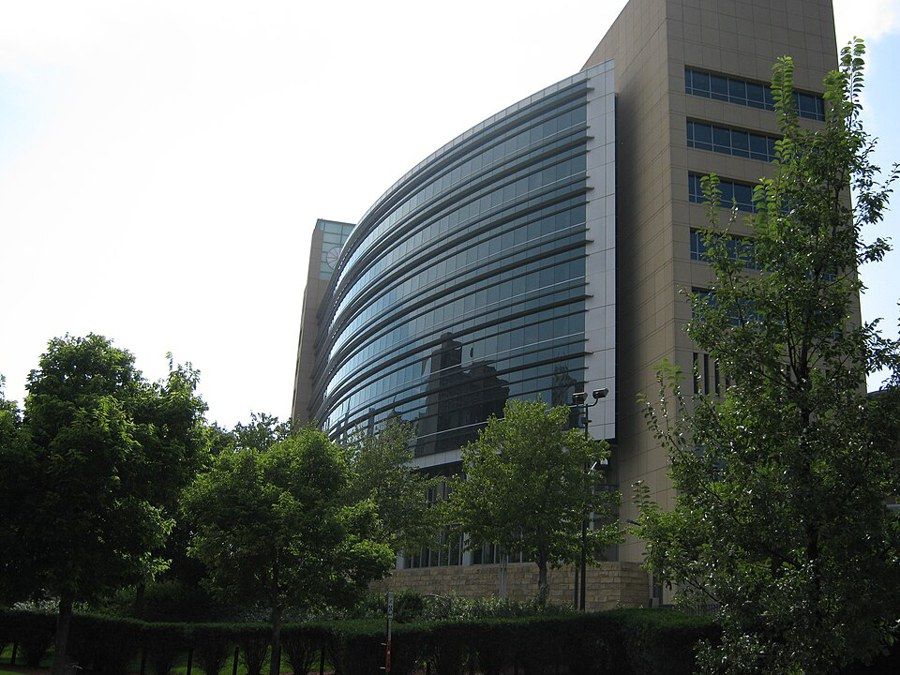
\includegraphics[height=0.34\textheight]{ch5_minneapolis_fed_2010.jpg}\\[1mm]
\imgcap{Federal Reserve Bank of Minneapolis, 2010}
\imgcredit{https://commons.wikimedia.org/wiki/File:Federal_Reserve_Bank_of_Minneapolis_building_2.jpg}{Foto: Innotata (2010); CC BY-SA 3.0; Wikimedia Commons}
\end{column}
\begin{column}{0.58\textwidth}
\begin{itemize}
    \item Începutul anilor 1980: Litterman realizează prognoze cu VAR bayesiene la Fed Minneapolis \refLit; distribuția a priori „Minnesota”
    \begin{itemize}
        \item \refDLS: suma coeficienților și proiecții condiționate; \refSims, \refSZ: observația inițială fictivă
    \end{itemize}
    \item 1989--2002: indici factoriali dinamici \refSWd, factori dinamici generalizați \refFHLR, indici de difuziune \refSWa
    \item 2005--2015: FAVAR \refBBE, nowcasting \refGRS, BVAR mari \refBGR, distribuții a priori ierarhice \refGLP
    \item O singură idee: cînd parametrii depășesc observațiile, adăugăm informație (o distribuție a priori) sau reducem dimensiunea (factori)
\end{itemize}
\end{column}
\end{columns}
\end{frame}


%=============================================================================
\section{Blestemul dimensionalității}
%=============================================================================

\begin{frame}{Numărarea parametrilor}
\itemsize{\small}
\begin{itemize}
    \item VAR($p$) cu $n$ variabile: $k = np + 1$ regresori pe ecuație, $nk$ coeficienți și $n(n + 1)/2$ covarianțe
    \begin{itemize}
        \item $n = 3$, $p = 13$: $k = 40$; $n = 20$: $k = 261$; $n = 102$: $k = 1\,327$ pe ecuație
        \item o fereastră de 10 ani are $T = 120$ de luni: cu $k > T$, OLS nu există ($X'X$ este singulară)
    \end{itemize}
    \item Chiar cu $k < T$, eroarea de estimare crește cu $k/T$: MSE la un pas $\approx \sigma^2(1 + k/T)$ pentru o regresie corect specificată
    \begin{itemize}
        \item supraajustare: potrivirea în eșantion se îmbunătățește, acuratețea în afara eșantionului se deteriorează
    \end{itemize}
    \item Trei remedii: (i) shrinkage (distribuții a priori bayesiene, ridge, LASSO); (ii) reducerea dimensiunii (factori); (iii) selecția variabilelor
\end{itemize}
\end{frame}

\begin{frame}{Simulare: VAR estimat prin OLS comparat cu un BVAR Minnesota}
\itemsize{\footnotesize}
\begin{center}
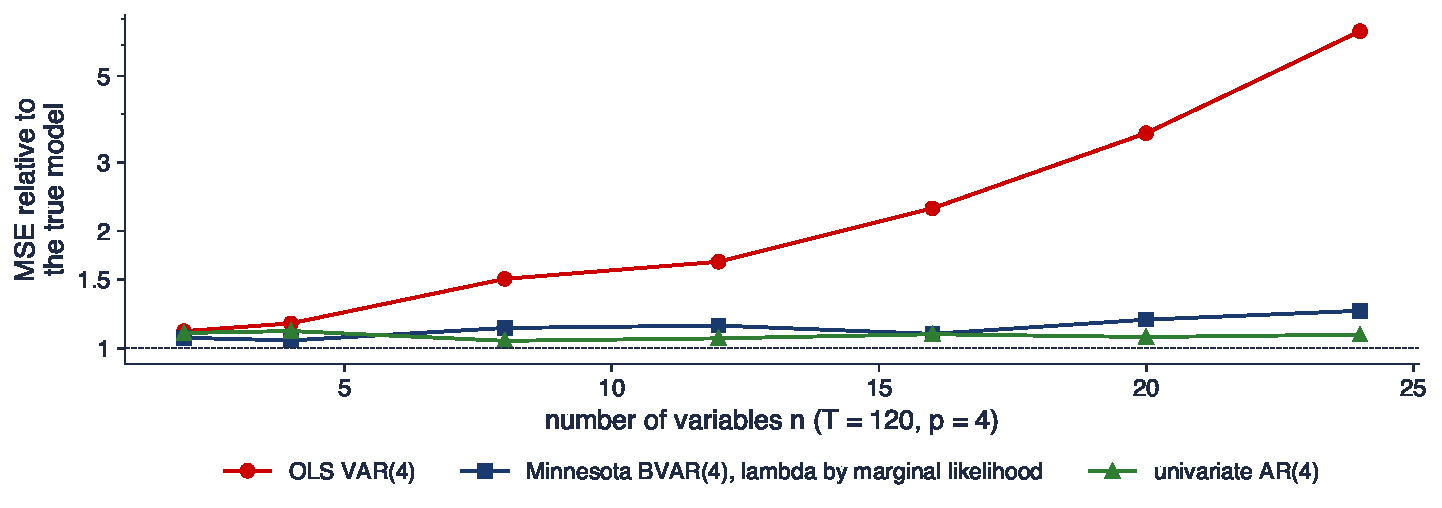
\includegraphics[width=0.97\textwidth,height=0.5\textheight,keepaspectratio]{ats_ch5_curse.pdf}
\end{center}
\vspace{-0.25cm}
\begin{itemize}
    \item Modelul adevărat: VAR(1) staționar $A = 0{,}5I + (0{,}3/n)\mathbf{1}\mathbf{1}'$; se estimează un VAR(4), $T = 120$; MSE la un pas al variabilei 1 raportat la modelul adevărat; 200 de replicări
\end{itemize}
\quantlet{ATS\_ch5\_bvar}{\qlurl{ATS_ch5_bvar}}
\end{frame}

\begin{frame}{Interpretarea simulării}
\itemsize{\small}
\begin{itemize}
    \item OLS: MSE relativ urcă la 6{,}52 pentru $n = 24$ ($k = 97$ de regresori pentru 116 observații)
    \item BVAR: 1{,}25 pentru $n = 24$; gradul de strîngere ales prin verosimilitatea marginală scade de la 0{,}31 ($n = 2$) la 0{,}14 ($n = 24$)
    \item Un AR(4) univariat rămîne în jurul valorii 1{,}08: informația dintre variabile există, dar este mică, iar OLS o risipește pe zgomot
    \item Cu cît sistemul este mai mare, cu atît distribuția a priori trebuie să fie mai strînsă: tema întregului capitol \refDGRa
\end{itemize}
\end{frame}

\begin{frame}{Recapitulare: blestemul dimensionalității}
\itemsize{\small}
\begin{itemize}
    \item Parametrii cresc cu $n^2p$; observațiile nu
    \item Shrinkage-ul schimbă o deplasare mică pe o reducere mare a varianței
    \item Factorii rezumă multe serii prin cîteva componente comune
\end{itemize}
\end{frame}


%=============================================================================
\section{Inferența bayesiană: ce ne trebuie}
%=============================================================================

\begin{frame}{Distribuția a priori, verosimilitatea, distribuția a posteriori}
\itemsize{\footnotesize}
\begin{columns}[T]
\begin{column}{0.34\textwidth}
\centering
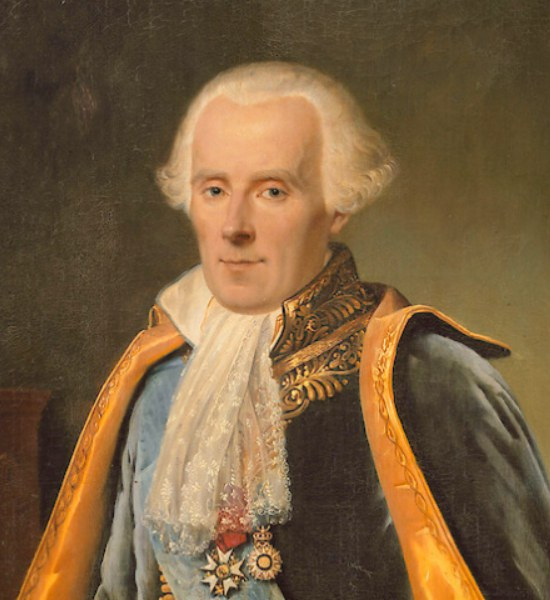
\includegraphics[height=0.36\textheight]{ch5_laplace_guerin_1838.jpg}\\[1mm]
\imgcap{Pierre-Simon Laplace, care a dezvoltat probabilitatea inversă}
\imgcredit{https://commons.wikimedia.org/wiki/File:Pierre-Simon_Laplace.jpg}{Portret: Paulin Guérin (1838); domeniu public; Wikimedia Commons}
\end{column}
\begin{column}{0.64\textwidth}
\begin{itemize}
    \item Bayes: $p(\theta\mid y) = p(y\mid\theta)p(\theta)/p(y)$, cu $p(y) = \int p(y\mid\theta)p(\theta)\,d\theta$
    \begin{itemize}
        \item $p(\theta)$: distribuția \textbf{a priori}; $p(y\mid\theta)$: verosimilitatea; $p(\theta\mid y)$: distribuția \textbf{a posteriori}
        \item $p(y)$: \textbf{verosimilitatea marginală}, evidența în favoarea modelului și a distribuției a priori
    \end{itemize}
    \item Conjugarea: distribuția a priori și cea a posteriori sînt din aceeași familie, deci cea a posteriori are formă închisă
    \begin{itemize}
        \item media distribuției Normale cu varianța cunoscută: Normală; coeficienți și varianță în regresie: Normal--inverse-gamma
    \end{itemize}
    \item Rezumate punctuale: media a posteriori (pierdere pătratică), mediana (pierdere absolută); mulțimi credibile din cuantilele a posteriori
\end{itemize}
\end{column}
\end{columns}
\end{frame}

\begin{frame}{Actualizarea Normală este o medie ponderată cu precizii}
\itemsize{\small}
\begin{itemize}
    \item Datele: $\hat\beta\mid\beta \sim N(\beta, s^2)$ cu $s^2 = \sigma^2/\sum x_t^2$; distribuția a priori: $\beta \sim N(m_0, v_0)$
    \begin{itemize}
        \item completăm pătratul în $\beta$: $\beta\mid y \sim N(m_1, v_1)$, $v_1^{-1} = v_0^{-1} + s^{-2}$
        \item $m_1 = w\,m_0 + (1 - w)\hat\beta$ cu $w = v_0^{-1}/(v_0^{-1} + s^{-2})$: preciziile se adună, mediile se mediază
    \end{itemize}
    \item În forma de regresie: $\bar\beta = (V_0^{-1} + X'X/\sigma^2)^{-1}(V_0^{-1}m_0 + X'y/\sigma^2)$
    \begin{itemize}
        \item cu $m_0 = 0$ și $V_0 = \tau^2I$ aceasta este regresia ridge cu penalizarea $\sigma^2/\tau^2$
        \item cînd $T \to \infty$, $X'X$ crește și ponderea distribuției a priori $w \to 0$: distribuția a priori contează în eșantioane mici și în modele mari
    \end{itemize}
    \item Seminarul 5, A1: actualizarea de mînă și alegerea bayesiană empirică a lui $\tau^2$
\end{itemize}
\end{frame}

\begin{frame}{Actualizarea unui coeficient AR(1)}
\itemsize{\footnotesize}
\begin{center}
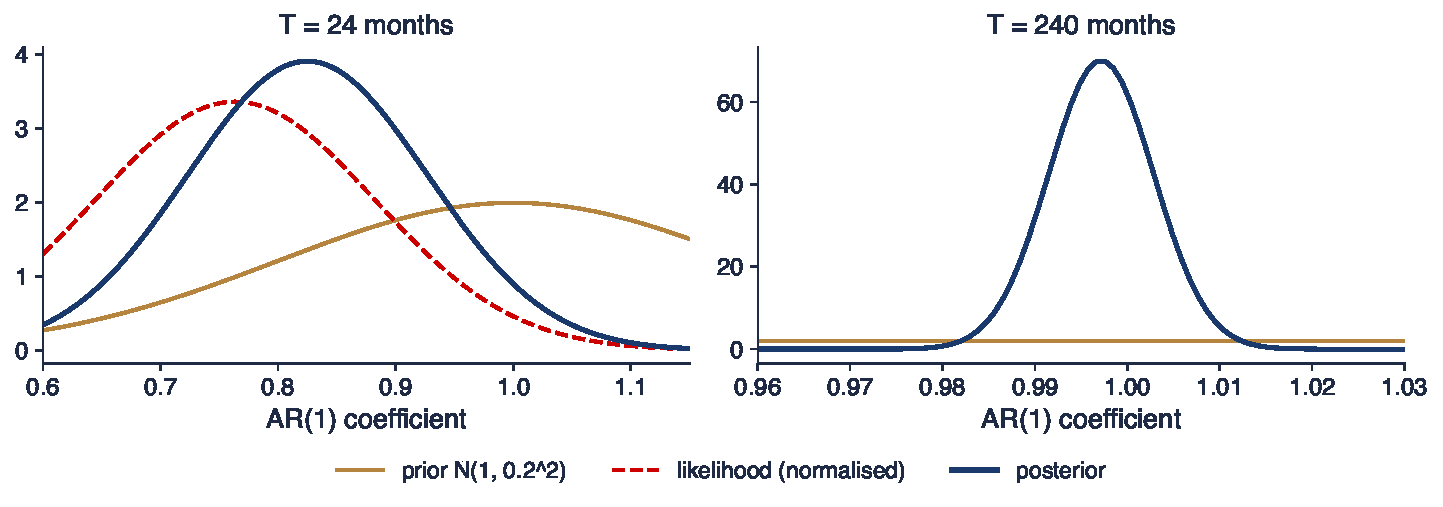
\includegraphics[width=0.97\textwidth,height=0.5\textheight,keepaspectratio]{ats_ch5_conjugate.pdf}
\end{center}
\vspace{-0.25cm}
\begin{itemize}
    \item Rata șomajului din SUA, lunar, ferestre care se încheie în decembrie 2019; distribuția a priori $N(1, 0{,}2^2)$ (mers aleator), $\sigma^2$ la estimația OLS
\end{itemize}
\quantlet{ATS\_ch5\_bayes}{\qlurl{ATS_ch5_bayes}}
\end{frame}

\begin{frame}{Interpretarea actualizării}
\itemsize{\small}
\begin{itemize}
    \item $T = 24$: OLS 0{,}763 (SE 0{,}119), media a posteriori 0{,}825 (abaterea standard 0{,}102); distribuția a priori are ponderea 26{,}0\%
    \item $T = 240$: OLS 0{,}997, a posteriori 0{,}997; ponderea distribuției a priori scade la 0{,}1\%
    \item Într-un VAR, fiecare ecuație are sute de coeficienți, dar același $T$: distribuția a priori păstrează ponderea pe care o are aici la $T = 24$
\end{itemize}
\end{frame}

\begin{frame}{Verosimilitatea marginală și factorii Bayes}
\itemsize{\small}
\begin{itemize}
    \item $p(y\mid M) = \int p(y\mid\theta, M)p(\theta\mid M)\,d\theta$: densitatea datelor \emph{înainte} de a le vedea
    \begin{itemize}
        \item descompunerea erorilor de predicție: $\ln p(y) = \sum_t \ln p(y_t\mid y_{1:t-1})$, o sumă de scoruri logaritmice la un pas (\atschlink{https://danpele.github.io/Advanced-Time-Series/RO/Cursuri/capitol1_evaluarea_prognozelor.pdf}{Capitolul 1})
        \item penalizează automat complexitatea: o distribuție a priori difuză împrăștie probabilitatea pe date care nu apar
    \end{itemize}
    \item Factorul Bayes $B_{12} = p(y\mid M_1)/p(y\mid M_2)$; $2\ln B_{12} > 6$ este o evidență „puternică” \refKR
    \begin{itemize}
        \item este sensibil la distribuția a priori: cu o distribuție a priori improprie nu este definit
    \end{itemize}
    \item Folosirea ierarhică: tratăm hiperparametrii $\gamma$ ai distribuției a priori ca parametri și maximizăm $p(y\mid\gamma)$ (Bayes empiric) sau le dăm o distribuție a priori \refGLP
\end{itemize}
\end{frame}

\begin{frame}{Eșantionarea Gibbs}
\itemsize{\small}
\begin{itemize}
    \item Cînd distribuția a posteriori comună nu are formă închisă, dar fiecare \textbf{distribuție condiționată completă} are: extragem $\theta_1\mid\theta_2, y$, apoi $\theta_2\mid\theta_1, y$ și repetăm \refGG, \refGS
    \begin{itemize}
        \item extragerile formează un lanț Markov a cărui distribuție staționară este cea a posteriori
        \item eliminăm o perioadă inițială (burn-in), apoi mediem funcții ale extragerilor (teorema ergodică)
    \end{itemize}
    \item Regresie cu distribuții a priori independente $\beta \sim N(b_0, V_0)$, $\sigma^2 \sim IG(a_0, d_0)$:
    \begin{itemize}
        \item $\beta\mid\sigma^2, y \sim N(\bar b, \bar V)$, $\bar V = (V_0^{-1} + X'X/\sigma^2)^{-1}$, $\bar b = \bar V(V_0^{-1}b_0 + X'y/\sigma^2)$
        \item $\sigma^2\mid\beta, y \sim IG(a_0 + T/2,\ d_0 + e'e/2)$ cu $e = y - X\beta$
    \end{itemize}
    \item În VAR: volatilitatea stochastică, distribuțiile a priori neconjugate și SVAR identificate pe mulțimi (\atschlink{https://danpele.github.io/Advanced-Time-Series/RO/Cursuri/capitol3_modele_var_structurale_proiectii_locale.pdf}{Capitolul 3}) cer pași Gibbs sau Metropolis--Hastings
\end{itemize}
\end{frame}

\begin{frame}{Diagnosticarea MCMC}
\itemsize{\small}
\begin{itemize}
    \item \textbf{Mărimea efectivă a eșantionului}: $\mathrm{ESS} = M/(1 + 2\sum_{k\ge1}\rho_k)$, cu $\rho_k$ autocorelațiile extragerilor
    \begin{itemize}
        \item lanț de tip AR(1): $\mathrm{ESS} = M(1 - \rho)/(1 + \rho)$; $\rho = 0{,}9$ păstrează aproximativ 5\% din extrageri
    \end{itemize}
    \item \textbf{$\widehat R$} \refGR: mai multe lanțuri din puncte de pornire dispersate; $\widehat R = \sqrt{\hat V/W}$, $\hat V = \frac{n-1}{n}W + B/n$
    \begin{itemize}
        \item $W$: varianța în interiorul lanțurilor, $B$: $n\times$ varianța mediilor lanțurilor; practica actuală: $\widehat R$ cu ranguri normalizate și lanțuri divizate $< 1{,}01$ \refVGS
    \end{itemize}
    \item Statistica $z$ \textbf{Geweke}: compară media primelor 10\% și a ultimelor 50\% din lanț, cu varianțe spectrale
    \item Niciuna nu demonstrează convergența; fiecare poate dezvălui un eșec
\end{itemize}
\end{frame}

\begin{frame}{Eșantionarea Gibbs: o parametrizare proastă și una bună}
\itemsize{\footnotesize}
\begin{center}
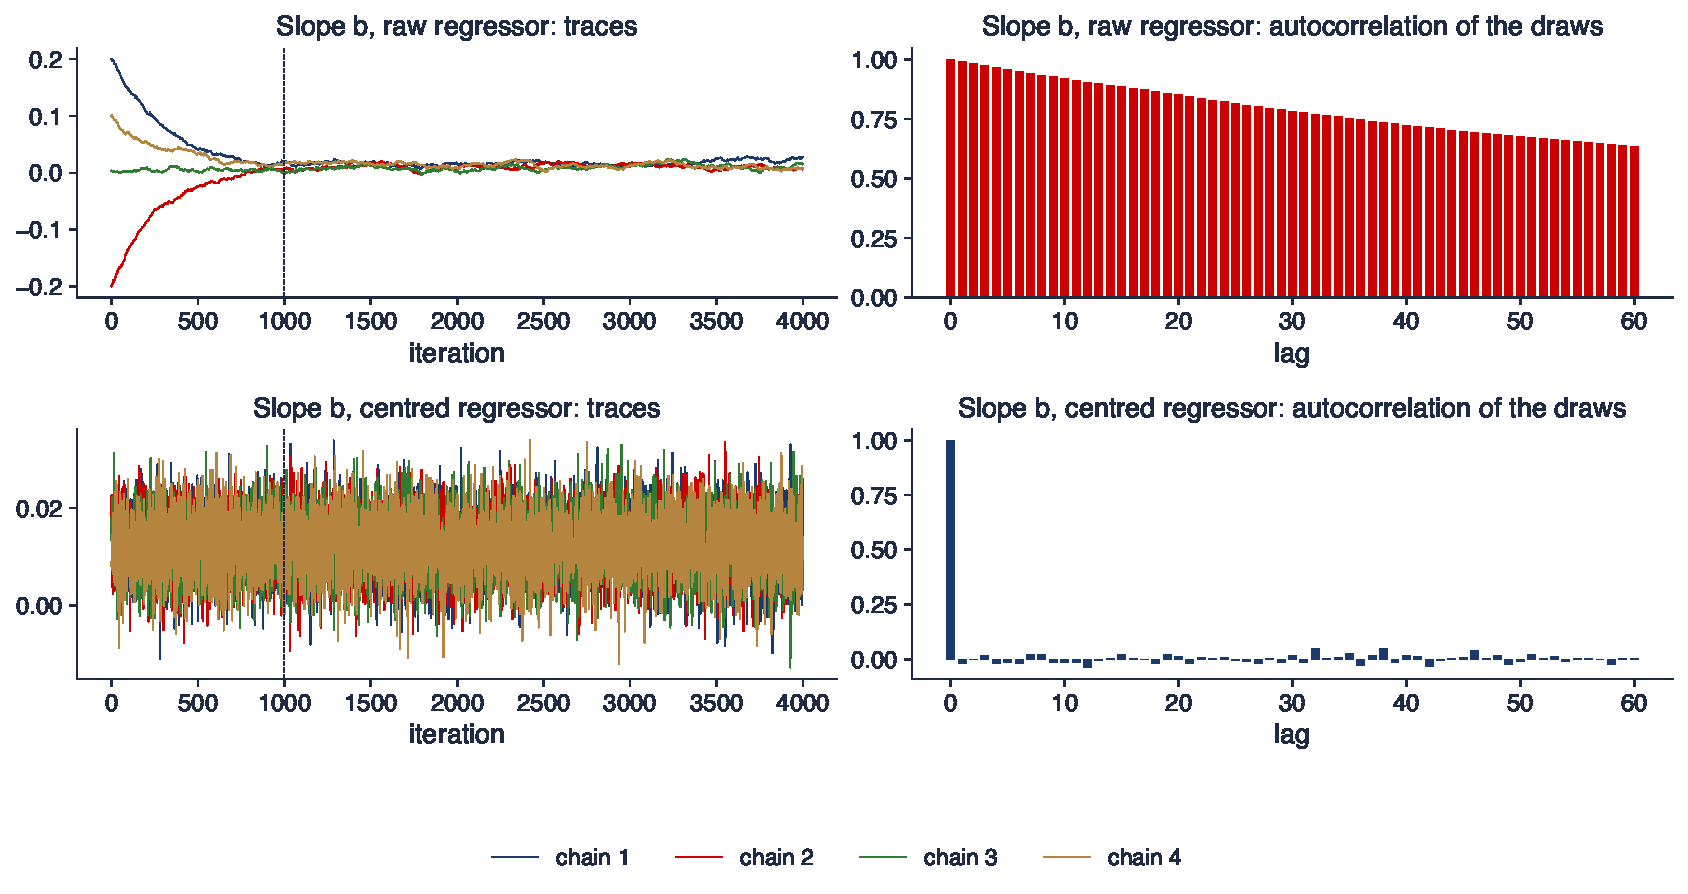
\includegraphics[width=0.97\textwidth,height=0.56\textheight,keepaspectratio]{ats_ch5_gibbs.pdf}
\end{center}
\vspace{-0.25cm}
\begin{itemize}
    \item Creșterea lunară a IP din SUA pe gradul de utilizare a capacităților decalat (media 79{,}0\%, abaterea standard 4{,}7), 1967--2019, $T = 635$; Gibbs pe cîte un parametru, patru lanțuri, 4\,000 de extrageri, burn-in 1\,000
\end{itemize}
\quantlet{ATS\_ch5\_bayes}{\qlurl{ATS_ch5_bayes}}
\end{frame}

\begin{frame}{Interpretarea celor două eșantionatoare}
\itemsize{\small}
\begin{itemize}
    \item Regresorul brut: corelația a posteriori dintre termenul liber și pantă este \ensuremath{-}0{,}998, deci fiecare pas condiționat se mișcă foarte puțin
    \begin{itemize}
        \item autocorelația de ordinul 1 0{,}992; ESS = 53 din 12\,000 de extrageri; $\widehat R$ = 1{,}32; $z$ Geweke = \ensuremath{-}2{,}27
    \end{itemize}
    \item Regresorul centrat: corelația \ensuremath{-}0{,}001, ESS = 11\,529, $\widehat R$ = 1{,}00, $z$ Geweke = 0{,}01
    \begin{itemize}
        \item același model, aceeași distribuție a posteriori a pantei (media 0{,}0123); s-a schimbat doar eșantionatorul
    \end{itemize}
    \item Lecția: reparametrizați sau extrageți împreună blocurile corelate; BVAR-urile conjugate evită problema extrăgînd $B$ într-un singur bloc
\end{itemize}
\end{frame}

\begin{frame}{Recapitulare: inferența bayesiană}
\itemsize{\small}
\begin{itemize}
    \item Precizia a posteriori = precizia a priori + precizia datelor; media este o medie ponderată
    \item Verosimilitatea marginală evaluează un model împreună cu distribuția lui a priori și poate alege hiperparametri
    \item Eșantionarea Gibbs cere distribuțiile condiționate complete; verificați ESS, $\widehat R$ și Geweke înainte de a avea încredere în extrageri
\end{itemize}
\end{frame}


%=============================================================================
\section{Distribuția a priori Minnesota și forma ei conjugată}
%=============================================================================

\begin{frame}{Distribuția a priori Minnesota}
\itemsize{\small}
\begin{itemize}
    \item Mediile a priori \refLit: $\E[(A_1)_{ii}] = \delta_i$, toți ceilalți coeficienți 0; $\delta_i = 1$ (mers aleator) pentru serii persistente, 0 (zgomot alb) în rest
    \begin{itemize}
        \item varianțele a priori \refBGR, ec.~(2): $\Var[(A_l)_{ij}] = \lambda^2/l^2$ dacă $j = i$, $\vartheta\lambda^2\sigma_i^2/(l^2\sigma_j^2)$ dacă $j \ne i$
    \end{itemize}
    \item Hiperparametri: $\lambda$ gradul general de strîngere, $1/l^2$ descreșterea cu decalajul, $\vartheta \in (0, 1]$ shrinkage-ul între variabile
    \begin{itemize}
        \item $\sigma_i^2$: varianța reziduală a unui AR univariat pentru $y_i$, astfel încît $\sigma_i^2/\sigma_j^2$ fixează unitățile de măsură
        \item $\lambda = 0$: a posteriori = a priori; $\lambda \to \infty$: media a posteriori = OLS
    \end{itemize}
    \item Versiunea originală: $\Sigma$ diagonală și fixă, fiecare ecuație o regresie separată de tip ridge, cu termen liber difuz
\end{itemize}
\end{frame}

\begin{frame}{Distribuția a priori natural conjugată}
\itemsize{\small}
\begin{itemize}
    \item Regresia multivariată $Y = XB + U$, liniile lui $U$ i.i.d.\ $N(0, \Sigma)$; distribuția a priori \refKK: $\mathrm{vec}(B)\mid\Sigma \sim N(\mathrm{vec}(B_0), \Sigma\otimes\Omega_0)$, $\Sigma \sim IW(\Psi, d)$
    \begin{itemize}
        \item a posteriori: $\bar\Omega^{-1} = \Omega_0^{-1} + X'X$, $\bar B = \bar\Omega(\Omega_0^{-1}B_0 + X'Y)$
        \item $\Sigma\mid Y \sim IW(\bar\Psi, T + d)$, $\bar\Psi = \Psi + \hat U'\hat U + (\bar B - B_0)'\Omega_0^{-1}(\bar B - B_0)$, $\hat U = Y - X\bar B$
    \end{itemize}
    \item Prețul conjugării: structura Kronecker dă fiecărei ecuații același $\Omega_0$, deci $\vartheta = 1$
    \begin{itemize}
        \item momentele Minnesota cu $\Omega_0 = \mathrm{diag}(\lambda^2/(l^2\sigma_j^2))$ și $\E\Sigma = \mathrm{diag}(\sigma_i^2)$ ($d = n + 2$, $\Psi = \mathrm{diag}(\sigma_i^2)$)
    \end{itemize}
    \item Cîștigul: o singură inversare $k\times k$ pentru toate ecuațiile; extrageri exacte fără MCMC; verosimilitatea marginală în formă închisă (\atsapplink{atsapp1}{atssrc1}{anexă})
\end{itemize}
\end{frame}

\begin{frame}{Observații fictive}
\itemsize{\small}
\begin{itemize}
    \item Estimarea mixtă Theil: adăugăm $T_d$ linii artificiale $(Y_d, X_d)$ și aplicăm OLS pe $\binom{Y_d}{Y}$, $\binom{X_d}{X}$
    \begin{itemize}
        \item echivalent cu distribuția a priori NIW cu $B_0 = (X_d'X_d)^{-1}X_d'Y_d$, $\Omega_0 = (X_d'X_d)^{-1}$ \refBGR, ec.~(5)
        \item blocul Minnesota: $Y_d = \mathrm{diag}(\delta_i\sigma_i)/\lambda$, $X_d = J_p\otimes\mathrm{diag}(\sigma_i)/\lambda$, $J_p = \mathrm{diag}(1, \dots, p)$
    \end{itemize}
    \item \textbf{Suma coeficienților} \refDLS: $Y_d = \mathrm{diag}(\bar y_i)/\mu$, $X_d = (\mathbf{1}_p'\otimes\mathrm{diag}(\bar y_i)/\mu,\ 0)$
    \begin{itemize}
        \item strînge $\Pi = I - \sum_l A_l$ spre 0 („diferențiere inexactă”): $\mu \to 0$ dă un VAR în diferențe, fără cointegrare
    \end{itemize}
    \item \textbf{Observația inițială fictivă} \refSims, \refSZ: o linie $y = \bar y'/\phi$, $x = (\bar y'/\phi, \dots, \bar y'/\phi, 1/\phi)$
    \begin{itemize}
        \item împinge spre rădăcini unitare \emph{sau} spre un model staționar cu media $\bar y$: permite cointegrarea (\atschlink{https://danpele.github.io/Advanced-Time-Series/RO/Cursuri/capitol4_cointegrare_vecm_ardl_panel.pdf}{Capitolul 4})
    \end{itemize}
\end{itemize}
\end{frame}

\begin{frame}{Cît shrinkage? Potrivirea în eșantion comparată cu acuratețea în afara eșantionului}
\itemsize{\footnotesize}
\begin{center}
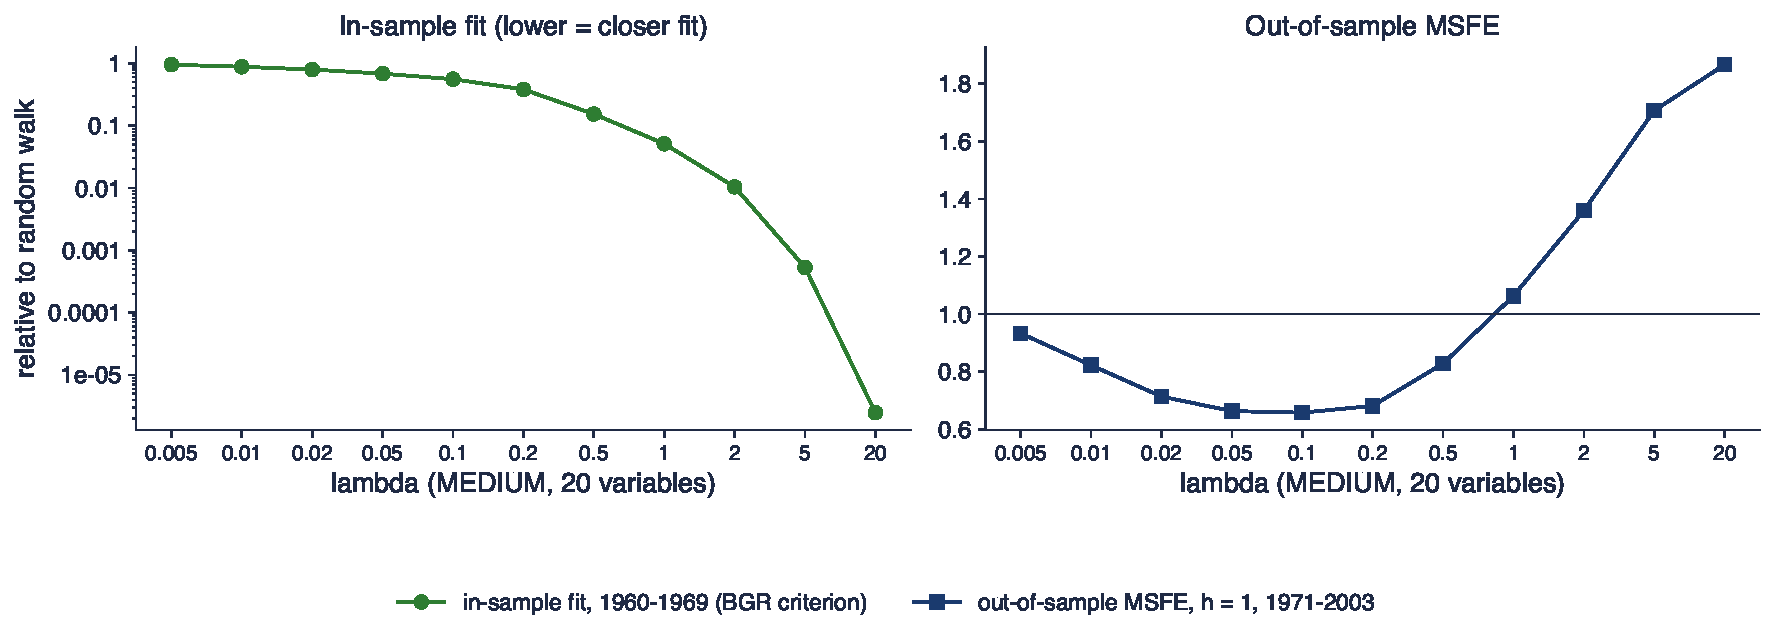
\includegraphics[width=0.97\textwidth,height=0.5\textheight,keepaspectratio]{ats_ch5_tradeoff.pdf}
\end{center}
\vspace{-0.25cm}
\begin{itemize}
    \item Sistemul MEDIUM (20 de variabile, $p = 13$, $k = 261$), distribuția a priori BGR, ferestre mobile de 10 ani; în afara eșantionului: MSFE la un pas pentru ocupare, IPC și dobînda federal funds, 1971--2003, relativ la mersul aleator
\end{itemize}
\quantlet{ATS\_ch5\_large\_bvar}{\qlurl{ATS_ch5_large_bvar}}
\end{frame}

\begin{frame}{Interpretarea compromisului}
\itemsize{\small}
\begin{itemize}
    \item Potrivirea în eșantion se îmbunătățește fără limită cînd $\lambda$ crește: cu $k = 261$ și $T = 120$, o distribuție a priori largă interpolează datele
    \item În afara eșantionului: formă de U; minimul 0{,}66 la $\lambda = 0{,}10$; 0{,}93 cu $\lambda = 0{,}005$ (aproape mersul aleator); 1{,}87 cu $\lambda = 20$
    \item Shrinkage-ul trebuie ales fără a privi eșantionul de evaluare: printr-o regulă de potrivire (BGR) sau prin verosimilitatea marginală (GLP)
\end{itemize}
\end{frame}

\begin{frame}{Recapitulare: distribuțiile a priori Minnesota și NIW}
\itemsize{\small}
\begin{itemize}
    \item Minnesota: centrăm fiecare ecuație pe un mers aleator sau pe zgomot alb; strîngem mai mult decalajele îndepărtate și celelalte variabile
    \item Forma natural conjugată păstrează formulele închise cu prețul $\vartheta = 1$
    \item Observațiile fictive implementează distribuția a priori prin OLS și adaugă convingeri despre suma coeficienților și observația inițială
\end{itemize}
\end{frame}


%=============================================================================
\section{Alegerea shrinkage-ului: distribuții a priori ierarhice}
%=============================================================================

\begin{frame}{Giannone, Lenza și Primiceri (2015)}
\itemsize{\small}
\begin{itemize}
    \item Tratăm $\gamma = (\lambda, \mu, \phi)$ ca parametri cu distribuții a priori proprii: $p(\gamma\mid y) \propto p(y\mid\gamma)p(\gamma)$ \refGLP
    \begin{itemize}
        \item $p(y\mid\gamma)$ este cunoscută în formă închisă pentru distribuția NIW cu observații fictive: datele plus observațiile fictive, minus observațiile fictive singure
        \item distribuții a priori pentru hiperparametri: Gamma cu modul 0,2 și abaterea standard 0,4 pentru $\lambda$, modul 1 și abaterea standard 1 pentru $\mu$ și $\phi$
    \end{itemize}
    \item Interpretare: verosimilitatea marginală este un scor în afara eșantionului al densităților predictive la un pas (secțiunea anterioară)
    \begin{itemize}
        \item deci echilibrează potrivirea și complexitatea fără un eșantion de evaluare
    \end{itemize}
    \item Folosim modul a posteriori al lui $\gamma$ (ca aici) sau integrăm $\gamma$ prin Metropolis--Hastings; GLP constată că ambele prognozează cam la fel de bine ca modelele factoriale
\end{itemize}
\end{frame}

\begin{frame}{Verosimilitatea marginală în funcție de gradul de strîngere}
\itemsize{\footnotesize}
\begin{center}
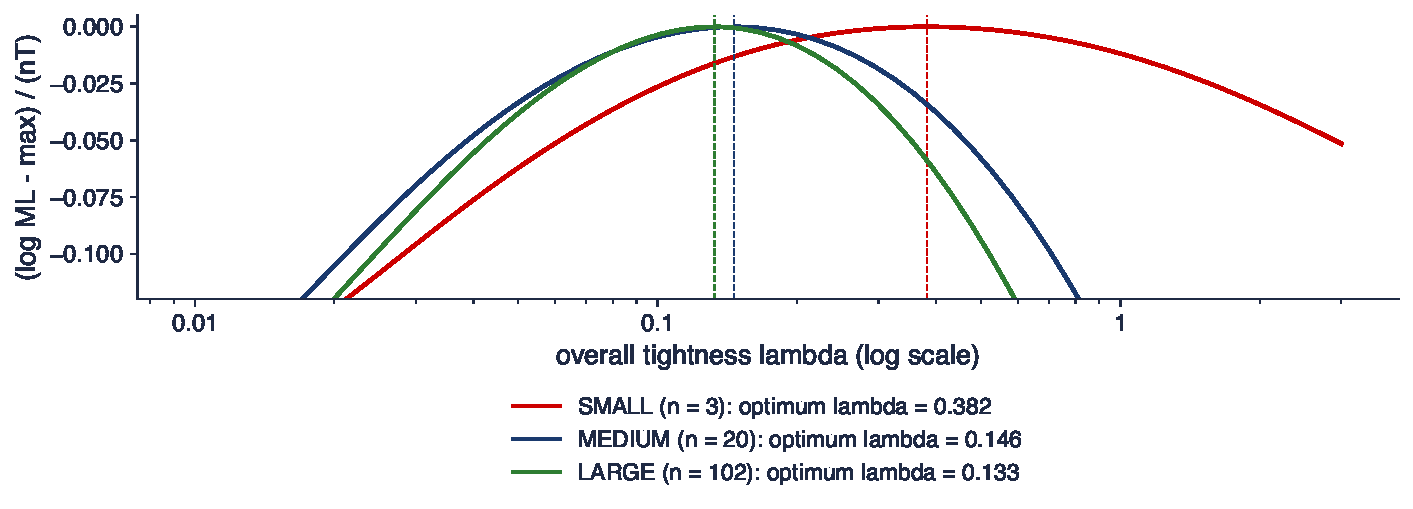
\includegraphics[width=0.97\textwidth,height=0.5\textheight,keepaspectratio]{ats_ch5_lambda.pdf}
\end{center}
\vspace{-0.25cm}
\begin{itemize}
    \item SMALL ($n = 3$), MEDIUM ($n = 20$), LARGE ($n = 102$), $p = 13$, 1960:1--2019:12 ($T = 707$); $\mu = \phi = 1$; log ML minus maximul, împărțit la $nT$
\end{itemize}
\quantlet{ATS\_ch5\_large\_bvar}{\qlurl{ATS_ch5_large_bvar}}
\end{frame}

\begin{frame}{Interpretarea verosimilității marginale}
\itemsize{\small}
\begin{itemize}
    \item Gradul optim de strîngere: 0{,}382 (SMALL), 0{,}146 (MEDIUM), 0{,}133 (LARGE): sistemele mai mari cer o distribuție a priori mai strînsă
    \item Valoarea din manuale $\lambda = 0{,}2$ costă \ensuremath{-}46{,}9 puncte logaritmice pentru MEDIUM și \ensuremath{-}597{,}2 pentru LARGE; $\lambda = 1$ costă \ensuremath{-}15571{,}6 pentru LARGE
    \item Modul comun cu distribuțiile hiperparametrilor: SMALL $\mu = 0{,}20$, $\phi = 0{,}44$; MEDIUM $\mu = 0{,}13$, $\phi = 0{,}44$: datele cer distribuții strînse pentru suma coeficienților și observația inițială
\end{itemize}
\end{frame}

\begin{frame}{Două reguli pentru un singur hiperparametru}
\itemsize{\small}
\begin{itemize}
    \item \textbf{Regula potrivirii BGR}: alegem $\lambda$ astfel încît potrivirea în eșantion la un pas a variabilelor-cheie să fie egală cu cea a unui VAR mic estimat prin OLS \refBGR, secțiunea~3
    \begin{itemize}
        \item $\mathrm{Fit}(\lambda) = \frac13\sum_{i\in I}\mathrm{msfe}_i^{(\lambda)}/\mathrm{msfe}_i^{(0)}$ pe 1960--1969; aici ținta este 0{,}43
        \item valorile noastre: MEDIUM 0{,}158, LARGE 0{,}059 (BGR, tabelul~1: 0,108 și 0,035 pe setul lor de date)
    \end{itemize}
    \item \textbf{Verosimilitatea marginală GLP}: reestimată pe fiecare fereastră; pe ferestre de 10 ani modul median este 0{,}34 (SMALL) și 0{,}28 (MEDIUM)
    \begin{itemize}
        \item intervalul 10\%--90\% al modului MEDIUM între ferestre: [0{,}23; 0{,}33]
    \end{itemize}
    \item Pachetul Python \texttt{bvar} al Băncii Angliei implementează optimizarea GLP pentru modelul conjugat; notebook-ul îl compară cu codul nostru \texttt{numpy}
\end{itemize}
\end{frame}

\begin{frame}{Recapitulare: distribuții a priori ierarhice}
\itemsize{\small}
\begin{itemize}
    \item Verosimilitatea marginală alege shrinkage-ul; acesta scade cînd sistemul crește
    \item Distribuțiile pentru suma coeficienților și observația inițială se aleg la fel
    \item O regulă de potrivire este o alternativă transparentă atunci cînd evaluarea trebuie să reproducă un studiu publicat
\end{itemize}
\end{frame}


%=============================================================================
\section{Studiu de caz: modele VAR bayesiene mari}
%=============================================================================

\begin{frame}{Bańbura, Giannone și Reichlin (2010): designul}
\itemsize{\small}
\begin{itemize}
    \item \refBGR: poate un VAR cu 131 de variabile să prognozeze și să identifice șocuri? Sistemele SMALL (ocupare, IPC, dobînda federal funds), MEDIUM (20), LARGE (toate)
    \begin{itemize}
        \item $p = 13$; ferestre mobile de 10 ani; prognoze punctuale din media a posteriori, iterate pînă la $h = 12$; reper: mers aleator cu derivă
        \item distribuția a priori NIW Minnesota plus suma coeficienților cu $\tau = 10\lambda$ (secțiunea~3.3); $\lambda$ prin regula potrivirii pe 1960--1969
    \end{itemize}
    \item Datele noastre: panelul în format FRED-MD; LARGE = cele 102 serii observate pe 1960--2026 (agregate și componente)
    \begin{itemize}
        \item MEDIUM: lista BGR, cu S\&P 500, cursul de schimb efectiv și rezervele neîmprumutate înlocuite de randamentul Baa, dobînda la 3 luni și autorizațiile de construcție (indisponibile pentru 1960--2026 sau negative după 2008)
    \end{itemize}
    \item Evaluarea: ținte 1971--2003 (lucrarea), 2004--2019 și 2004--2026 (extinderi); 678 de origini ale prognozelor; adăugăm GLP SMALL și MEDIUM
\end{itemize}
\end{frame}

\begin{frame}{Acuratețea prognozelor, 1971--2003}
\itemsize{\footnotesize}
\begin{center}
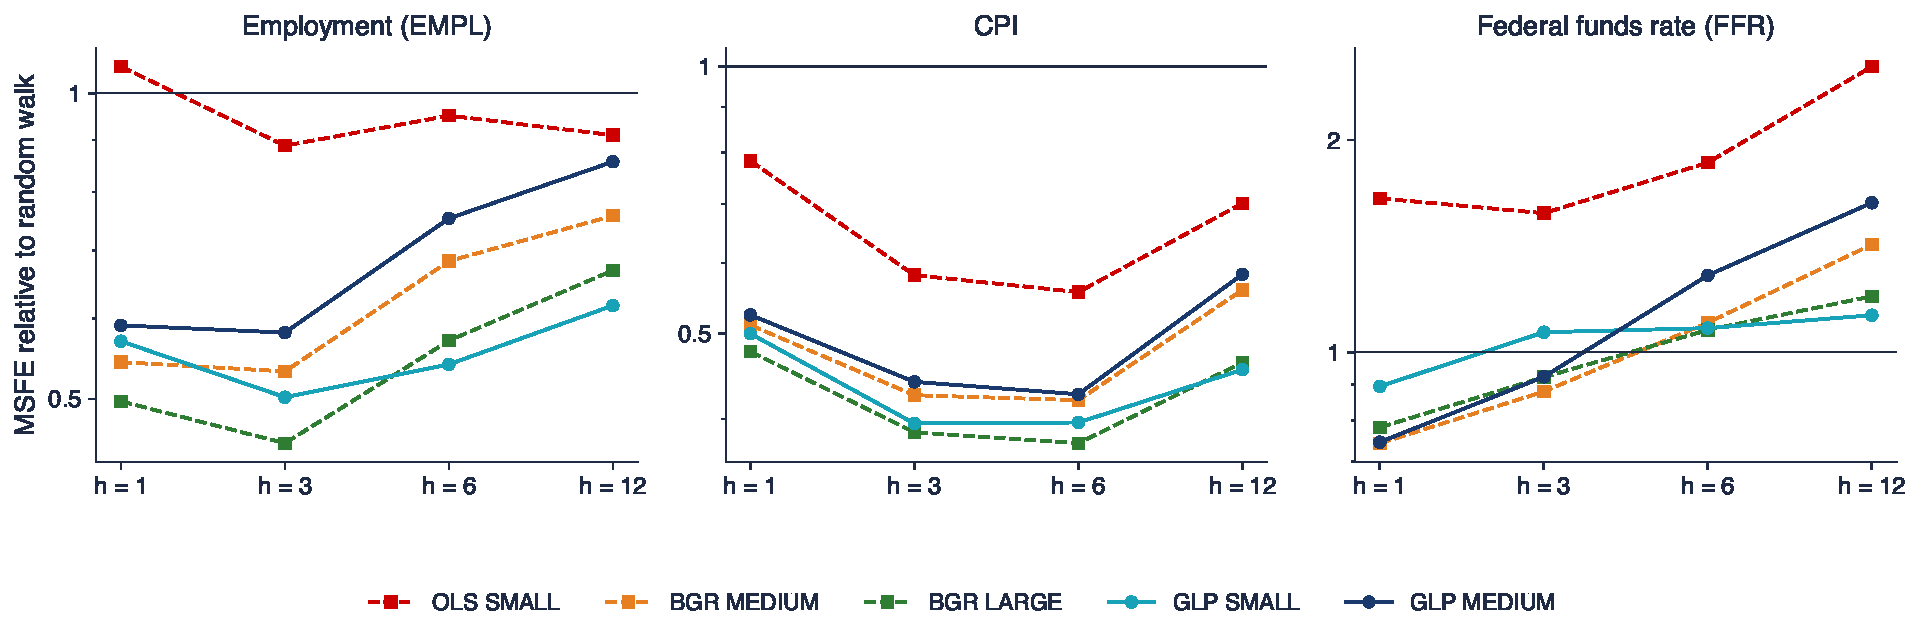
\includegraphics[width=0.97\textwidth,height=0.5\textheight,keepaspectratio]{ats_ch5_bgr.pdf}
\end{center}
\vspace{-0.25cm}
\begin{itemize}
    \item MSFE relativ la mersul aleator cu derivă (scară logaritmică; sub 1 = mai bine), ocuparea și IPC în 100 $\times$ logaritmul nivelului, dobînda în procente
\end{itemize}
\quantlet{ATS\_ch5\_large\_bvar}{\qlurl{ATS_ch5_large_bvar}}
\end{frame}

\begin{frame}{Interpretarea comparației prognozelor}
\itemsize{\small}
\begin{itemize}
    \item $h = 1$, ocuparea: OLS SMALL 1{,}06, BGR MEDIUM 0{,}54, LARGE 0{,}50 (BGR, tabelul~1: 1,14; 0,54; 0,46)
    \begin{itemize}
        \item IPC: 0{,}78; 0{,}51; 0{,}48; dobînda federal funds: 1{,}65; 0{,}74; 0{,}78
    \end{itemize}
    \item Adăugarea de variabile cu mai mult shrinkage ajută: LARGE bate SMALL pentru fiecare variabilă la $h \le 6$
    \item GLP SMALL este aproape la fel de bun ca sistemele mari pentru ocupare și IPC (0{,}57; 0{,}50): mare parte din cîștig vine din distribuția a priori, nu doar din variabile
    \item Dobînda federal funds după 3 luni este dificilă pentru toate modelele (LARGE 1{,}20 la $h = 12$)
\end{itemize}
\end{frame}

\begin{frame}{După 2003: extinderea și martie 2020}
\itemsize{\footnotesize}
\begin{center}
\scriptsize
\begin{tabular}{lcccccc}
\toprule
\textbf{Modelul} & \textbf{EMPL, 1} & \textbf{EMPL, 12} & \textbf{CPI, 1} & \textbf{CPI, 12} & \textbf{FFR, 1} & \textbf{FFR, 12} \\
\midrule
OLS SMALL & 0{,}38 & 1{,}08 & 1{,}26 & 2{,}43 & 0{,}98 & 3{,}51 \\
BGR MEDIUM & 0{,}20 & 0{,}66 & 0{,}97 & 6{,}49 & 0{,}55 & 1{,}91 \\
BGR LARGE & 0{,}19 & 0{,}67 & 0{,}92 & 3{,}73 & 0{,}45 & 1{,}79 \\
GLP SMALL & 0{,}24 & 0{,}33 & 0{,}93 & 1{,}07 & 0{,}61 & 0{,}67 \\
GLP MEDIUM & 0{,}20 & 0{,}28 & 0{,}95 & 2{,}55 & 0{,}57 & 0{,}91 \\
\bottomrule
\end{tabular}
\end{center}
\begin{itemize}
    \item Ținte 2004:1--2019:12, MSFE relativ (mersul aleator cu derivă = 1)
    \item Incluzînd 2020--2026, MSFE la 12 luni pentru ocupare explodează: BGR MEDIUM 500{,}06, GLP SMALL 8{,}64: ferestrele care conțin aprilie 2020 tratează prăbușirea ca dinamică
    \item Remediul: scalăm varianța reziduală a lunilor pandemiei cu factori estimați \refLP{} sau folosim volatilitatea stochastică (secțiunea următoare)
\end{itemize}
\end{frame}

\begin{frame}{Un șoc de politică monetară într-un VAR mare}
\itemsize{\small}
\begin{itemize}
    \item Schema recursivă din \refBGR, secțiunea~4: $y_t = (X_t, r_t, Z_t)$, variabile lente $X_t$ (activitate reală, prețuri), dobînda $r_t$, variabile rapide $Z_t$ (monedă, dobînzi, cursuri de schimb)
    \begin{itemize}
        \item contează doar poziția lui $r_t$ (\atschlink{https://danpele.github.io/Advanced-Time-Series/RO/Cursuri/capitol3_modele_var_structurale_proiectii_locale.pdf}{Capitolul 3}): nu este nevoie de nicio ordonare în interiorul blocurilor
    \end{itemize}
    \item Benzi bayesiene: pentru fiecare extragere $(B, \Sigma)$ din distribuția a posteriori NIW calculăm coloana de impact Cholesky și răspunsurile; raportăm cuantilele a posteriori
    \begin{itemize}
        \item 500 de extrageri, șoc de 100 bp, eșantion 1961--2002, $p = 13$; SMALL cu o distribuție a priori aproape plată
    \end{itemize}
    \item Acestea sînt benzile a posteriori anunțate în \atschlink{https://danpele.github.io/Advanced-Time-Series/RO/Cursuri/capitol3_modele_var_structurale_proiectii_locale.pdf}{Capitolul 3}: intervale credibile punctuale, condiționate de ipoteza de identificare
\end{itemize}
\end{frame}

\begin{frame}{Răspunsuri la un șoc de 100 bp al dobînzii federal funds}
\itemsize{\footnotesize}
\begin{center}
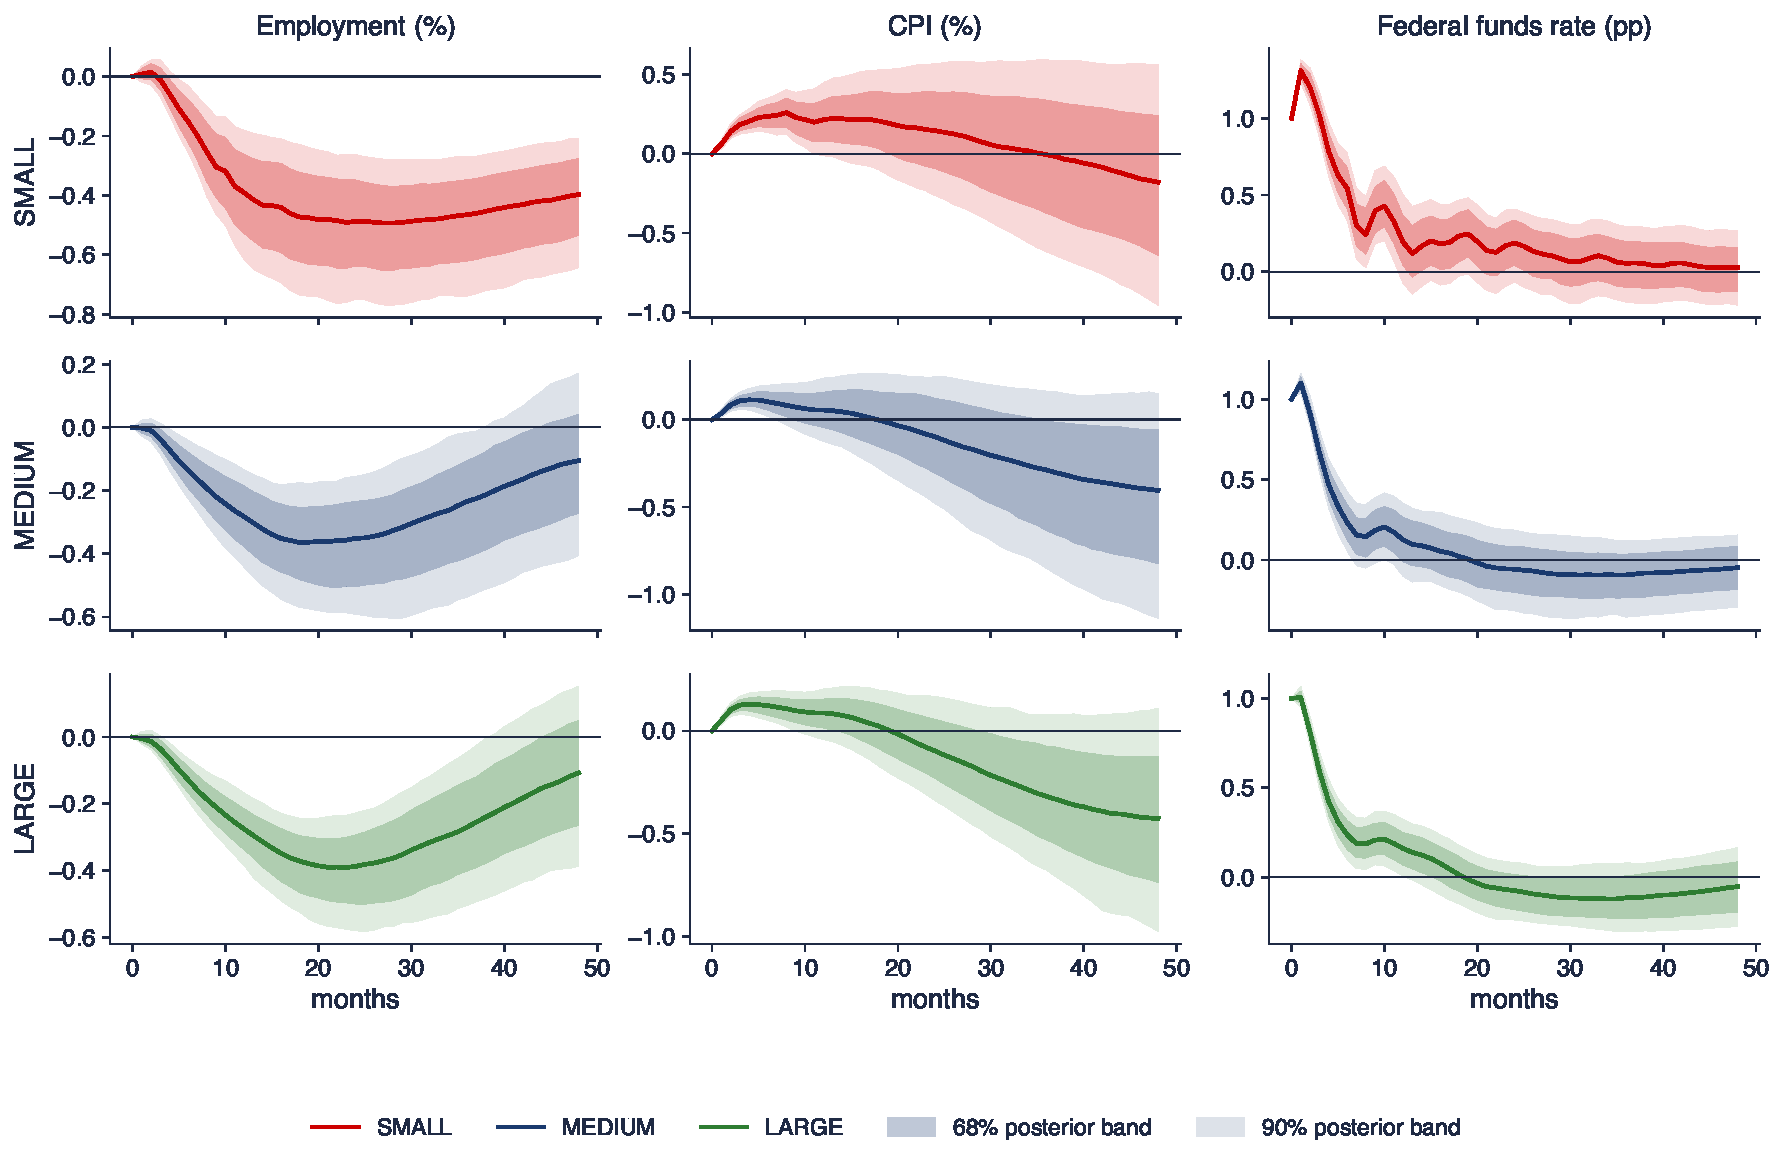
\includegraphics[width=0.97\textwidth,height=0.6\textheight,keepaspectratio]{ats_ch5_bvar_irf.pdf}
\end{center}
\vspace{-0.25cm}
\begin{itemize}
    \item Mediane a posteriori cu benzi de 68\% și 90\%; liniile: SMALL, MEDIUM, LARGE; ocuparea și IPC în procente
\end{itemize}
\quantlet{ATS\_ch5\_large\_bvar}{\qlurl{ATS_ch5_large_bvar}}
\end{frame}

\begin{frame}{Interpretarea răspunsurilor}
\itemsize{\small}
\begin{itemize}
    \item Ocuparea: minimum \ensuremath{-}0{,}49\% (SMALL, luna 28), \ensuremath{-}0{,}39\% (LARGE, luna 23); după patru ani LARGE revine la \ensuremath{-}0{,}11\% (banda [\ensuremath{-}0{,}39; 0{,}15])
    \item IPC: anomalia prețurilor scade de la 0{,}26\% (SMALL) la 0{,}13\% (LARGE); după patru ani LARGE dă \ensuremath{-}0{,}43\% (banda [\ensuremath{-}0{,}97; 0{,}11])
    \item Ca în BGR: mai multă informație face răspunsul ocupării mai puțin persistent și răspunsul prețurilor mai plauzibil
    \item Benzile nu se lărgesc cu 102 variabile: distribuția a priori plătește coeficienții suplimentari
\end{itemize}
\end{frame}

\begin{frame}{Recapitulare: modele BVAR mari}
\itemsize{\small}
\begin{itemize}
    \item Cu un shrinkage care crește odată cu sistemul, un VAR cu 102 variabile prognozează mai bine decît un VAR cu 3 variabile estimat prin OLS
    \item Rezultatele BGR pentru 1971--2003 se replică pe datele actuale; după 2020 BVAR-ul homoscedastic eșuează
    \item Seturile mari de informații reduc anomalia prețurilor din VAR-urile monetare mici
\end{itemize}
\end{frame}


%=============================================================================
\section{Volatilitate stochastică în modelele BVAR}
%=============================================================================

\begin{frame}{Modele BVAR mari cu volatilitate stochastică}
\itemsize{\small}
\begin{itemize}
    \item \textbf{Volatilitate comună} \refCCMa: $u_t = \sqrt{f_t}\,\varepsilon_t$, $\varepsilon_t \sim N(0, \Sigma)$, $\ln f_t = \phi\ln f_{t-1} + \nu_t$
    \begin{itemize}
        \item dat fiind $f_{1:T}$, modelul este un BVAR conjugat ponderat (liniile împărțite la $\sqrt{f_t}$); $f_t$ se extrage cu un pas Kim--Shephard--Chib
    \end{itemize}
    \item \textbf{Volatilități specifice fiecărei variabile} \refCCMb, \refClark: $\Sigma_t = A^{-1}H_tA^{-1\prime}$, $H_t$ diagonală cu volatilități log-AR \refPrim
    \begin{itemize}
        \item conjugarea se pierde; algoritmul triunghiular extrage ecuațiile una cîte una și face posibil $n = 100$
    \end{itemize}
    \item Cîștigurile: mai ales în prognozele de densitate (intervale calibrate) și în robustețea la valori extreme precum 2020
\end{itemize}
\end{frame}

\begin{frame}{Un factor comun de volatilitate în reziduurile BVAR}
\itemsize{\footnotesize}
\begin{center}
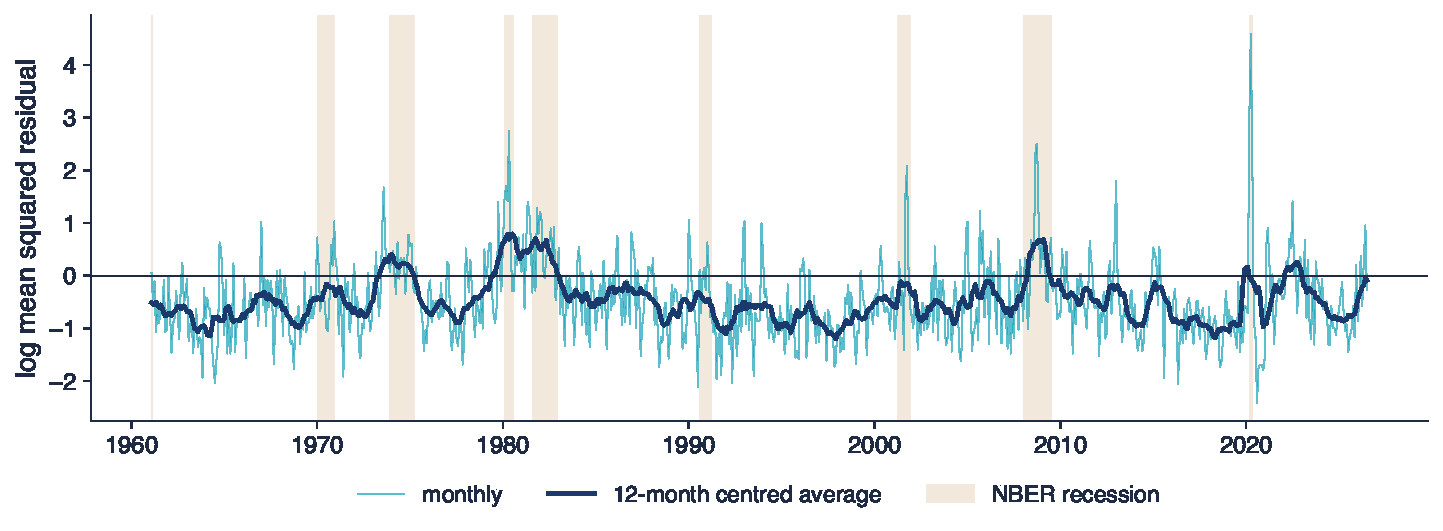
\includegraphics[width=0.97\textwidth,height=0.5\textheight,keepaspectratio]{ats_ch5_common_vol.pdf}
\end{center}
\vspace{-0.25cm}
\begin{itemize}
    \item BVAR MEDIUM (hiperparametri GLP), 1960--2026: logaritmul mediei transversale a pătratelor reziduurilor standardizate
\end{itemize}
\quantlet{ATS\_ch5\_large\_bvar}{\qlurl{ATS_ch5_large_bvar}}
\end{frame}

\begin{frame}{Interpretarea indicatorului de volatilitate}
\itemsize{\small}
\begin{itemize}
    \item Mișcări comune: varianța reziduală crește în fiecare recesiune și scade în Marea Moderație (1960--1984 este de 1{,}28 ori 1985--2007)
    \item Aprilie 2020 este de 176 ori luna mediană: un BVAR gaussian homoscedastic o tratează ca pe o observație obișnuită
    \item Acesta este argumentul pentru modelul cu volatilitate comună (o singură stare în plus) înaintea modelului complet cu volatilități specifice; \atschlink{https://danpele.github.io/Advanced-Time-Series/RO/Cursuri/capitol6_modele_spatiul_starilor_filtrare_bayesiana.pdf}{Capitolul 6} dă instrumentele de filtrare
\end{itemize}
\end{frame}


%=============================================================================
\section{Modele factoriale aproximative}
%=============================================================================

\begin{frame}{Modelul factorial aproximativ}
\itemsize{\small}
\begin{itemize}
    \item $x_{it} = \lambda_i'F_t + e_{it}$, $i = 1, \dots, N$, $t = 1, \dots, T$; $F_t$: $r$ factori comuni, $\lambda_i$: ponderi factoriale (loadings), $e_{it}$: componente idiosincratice
    \begin{itemize}
        \item \emph{aproximativ} \refCR: $e_{it}$ pot fi slab corelate între $i$ și în timp, cu condiția ca acea corelație să rămînă mărginită cînd $N \to \infty$
        \item caracterul general: $\Lambda'\Lambda/N \to \Sigma_\Lambda > 0$; cele mai mari $r$ valori proprii ale lui $XX'$ cresc cu $N$, celelalte nu
    \end{itemize}
    \item Identificarea: $\Lambda F_t = (\Lambda H)(H^{-1}F_t)$ pentru orice $H$ inversabilă: este identificat doar spațiul factorilor
    \begin{itemize}
        \item normalizarea pentru PCA: $F'F/T = I_r$ și $\Lambda'\Lambda$ diagonală
    \end{itemize}
    \item Forma statică a unui model dinamic: decalajele factorilor dinamici sînt așezate în $F_t$ \refSWc; modelul dinamic generalizat lucrează în domeniul frecvențelor \refFHLR
\end{itemize}
\end{frame}

\begin{frame}{Componente principale}
\itemsize{\small}
\begin{itemize}
    \item Cele mai mici pătrate: $\min_{F, \Lambda}\sum_{i,t}(x_{it} - \lambda_i'F_t)^2$ cu $F'F/T = I$: $\hat F = \sqrt T\times$ primii $r$ vectori proprii ai lui $XX'$, $\hat\Lambda = X'\hat F/T$
    \begin{itemize}
        \item standardizați întîi fiecare serie: PCA nu este invariantă la scară
    \end{itemize}
    \item Consistența \refSWa, \refBai: $\hat F_t \to HF_t$ cînd $N, T \to \infty$, cu viteza $\min(\sqrt N, \sqrt T)$
    \begin{itemize}
        \item dacă $\sqrt T/N \to 0$, factorii estimați pot fi folosiți ca regresori ca și cum ar fi observați (fără corecția pentru regresori generați)
    \end{itemize}
    \item Valori lipsă și date de început diferite: EM \refSWb, \refMN: completăm cu 0, aplicăm PCA, recompletăm celulele lipsă cu $\hat\lambda_i'\hat F_t$, iterăm
\end{itemize}
\end{frame}

\begin{frame}{Baza de date FRED-MD}
\itemsize{\small}
\begin{itemize}
    \item \refMN: aproximativ 130 de serii lunare SUA începînd din 1959, actualizate lunar, cu un cod de transformare pentru fiecare serie și cu ediții pentru analize în timp real
    \begin{itemize}
        \item opt grupe: producție și venit, piața muncii, locuințe, consum și comenzi, monedă și credit, dobînzi și cursuri de schimb, prețuri, piața de acțiuni
        \item valori extreme: o observație aflată la mai mult de 10 abateri intercuartilice de mediană devine lipsă (3 celule aici)
    \end{itemize}
    \item Panelul nostru: 117 serii FRED-MD distribuite de FRED (seriile bursiere nu sînt), 1960:1--2026:7, 4{,}5\% celule lipsă
    \begin{itemize}
        \item fișierul oficial (current.csv al St.~Louis Fed) îl poate înlocui în notebook printr-o singură linie
    \end{itemize}
    \item Doar ediția curentă: rezultatele sînt pseudo în afara eșantionului, nu în timp real \refCS
\end{itemize}
\end{frame}

\begin{frame}{Factorii panelului FRED-MD}
\itemsize{\footnotesize}
\begin{center}
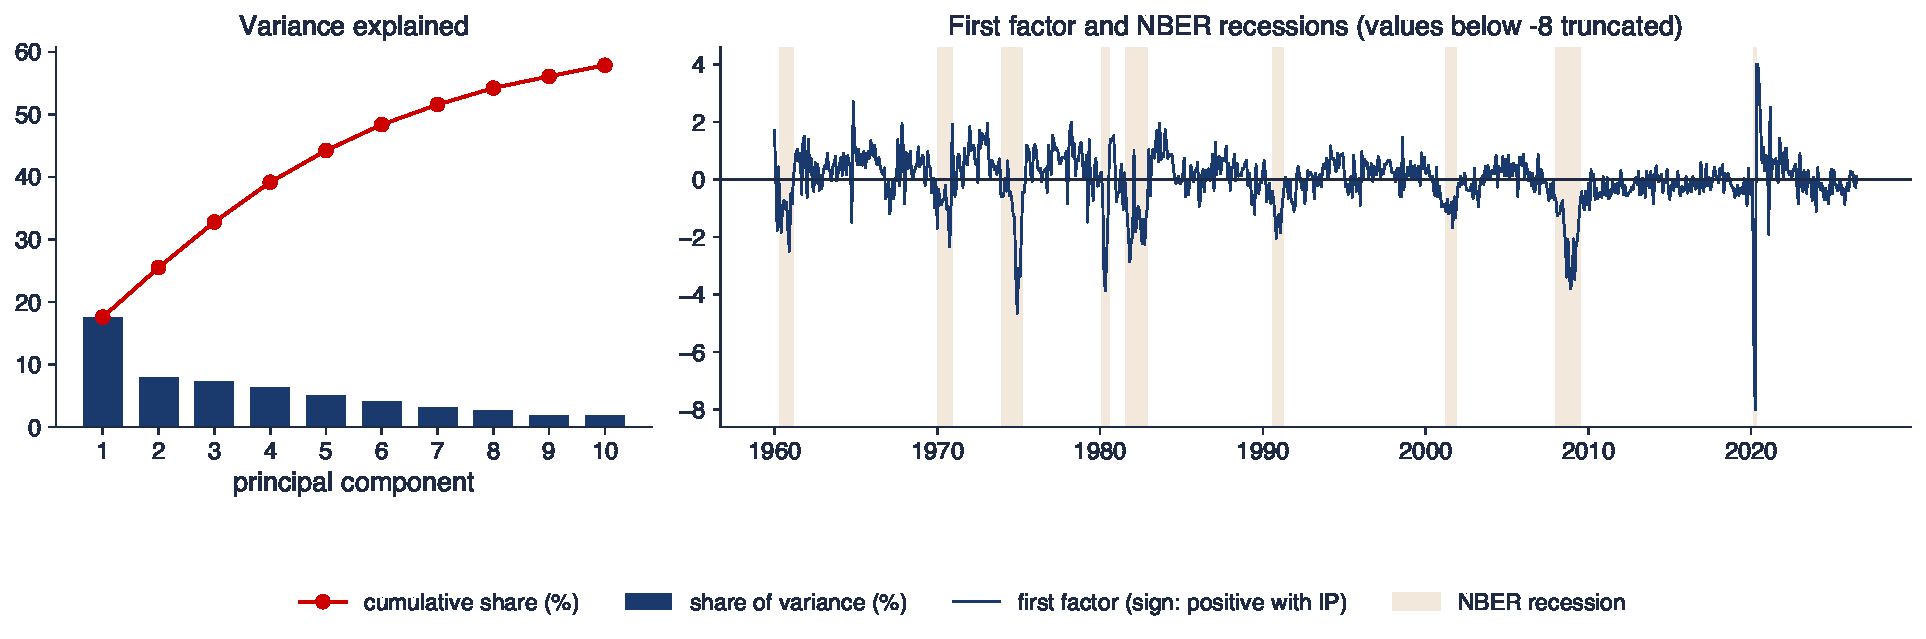
\includegraphics[width=0.97\textwidth,height=0.5\textheight,keepaspectratio]{ats_ch5_factors.pdf}
\end{center}
\vspace{-0.25cm}
\begin{itemize}
    \item Stînga: ponderea varianței panelului standardizat explicată de fiecare componentă principală; dreapta: primul factor (EM, 8 factori), recesiunile NBER marcate
\end{itemize}
\quantlet{ATS\_ch5\_factors}{\qlurl{ATS_ch5_factors}}
\end{frame}

\begin{frame}{Interpretarea factorilor}
\itemsize{\small}
\begin{itemize}
    \item Prima componentă explică 17{,}6\%, a doua 7{,}9\%; cinci explică 44{,}2\%, opt 54{,}2\%
    \item Primul factor este un indice al activității reale: corelația \ensuremath{-}0{,}58 cu indicatorul recesiunilor NBER; minimul este în aprilie 2020
    \item Nicio componentă nu domină: panelurile macro au cîțiva factori puternici și o coadă lungă de factori slabi, ceea ce face din numărul de factori o întrebare reală
\end{itemize}
\end{frame}

\begin{frame}{Cîți factori? Bai și Ng (2002)}
\itemsize{\small}
\begin{itemize}
    \item $V(k) = (NT)^{-1}\sum_{i,t}(x_{it} - \hat\lambda_i'\hat F_t)^2$ după $k$ componente; scade cu $k$, deci are nevoie de o penalizare \refBN
    \begin{itemize}
        \item $IC_{p1}(k) = \ln V(k) + k\frac{N + T}{NT}\ln\frac{NT}{N + T}$, $IC_{p2}(k) = \ln V(k) + k\frac{N + T}{NT}\ln C_{NT}^2$, $C_{NT}^2 = \min(N, T)$
        \item variantele $PC_{p}$: $V(k) + k\hat\sigma^2 g(N, T)$ cu $\hat\sigma^2 = V(k_{\max})$: depind de $k_{\max}$
    \end{itemize}
    \item Panelul nostru ($k_{\max} = 15$): $IC_{p1}$ = 8, $IC_{p2}$ = 8, $IC_{p3}$ = 10, $PC_{p1}$ = 13, $PC_{p2}$ = 11
    \begin{itemize}
        \item criteriile nu sînt de acord atunci cînd valorile proprii scad lent; raportați alegerea și sensibilitatea ei
    \end{itemize}
    \item Pentru prognoză, numărul de factori din regresie se alege separat (prin BIC), ca în prognozele cu indici de difuziune
\end{itemize}
\end{frame}

\begin{frame}{Conținutul economic al factorilor}
\itemsize{\footnotesize}
\begin{center}
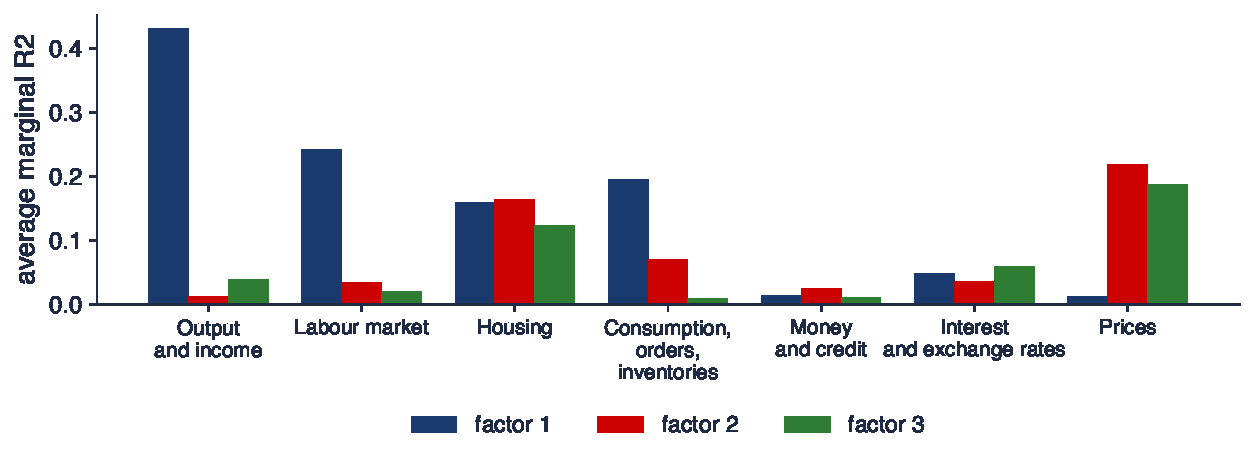
\includegraphics[width=0.97\textwidth,height=0.5\textheight,keepaspectratio]{ats_ch5_mr2.pdf}
\end{center}
\vspace{-0.25cm}
\begin{itemize}
    \item $R^2$ marginal mediu al regresiei fiecărei serii standardizate pe un singur factor, pe grupe (ca în McCracken și Ng 2016)
\end{itemize}
\quantlet{ATS\_ch5\_factors}{\qlurl{ATS_ch5_factors}}
\end{frame}

\begin{frame}{Interpretarea R2 marginal}
\itemsize{\small}
\begin{itemize}
    \item Factorul 1 este activitatea reală: $R^2$ 0{,}43 pentru producție, 0{,}24 pentru muncă; cea mai bine explicată serie are 0{,}78
    \item Factorii 2 și 3 se încarcă pe prețuri (0{,}22; 0{,}19) și pe locuințe (0{,}16; 0{,}12)
    \item Dobînzile se încarcă slab pe primii trei factori: informația monetară se află în factori ulteriori sau în dobînzile înseși, motivația pentru FAVAR
    \item Etichetele sînt o alegere de rotație: este identificat spațiul factorilor, nu fiecare factor
\end{itemize}
\end{frame}

\begin{frame}{Prognoze cu indici de difuziune: Stock și Watson (2002)}
\itemsize{\small}
\begin{itemize}
    \item \refSWb: $y_{t+h}^h = \alpha_h + \beta_h'\hat F_t + \sum_{j=0}^{p}\gamma_{hj}z_{t-j} + \varepsilon_{t+h}$ (prognoză directă, o ecuație pentru fiecare $h$)
    \begin{itemize}
        \item serii reale: $y_{t+h}^h = \frac{1200}{h}\ln(Y_{t+h}/Y_t)$; prețuri: $\frac{1200}{h}\ln(P_{t+h}/P_t) - 1200\ln(P_t/P_{t-1})$
        \item DI: doar factori, $k \in \{1, \dots, 12\}$ prin BIC; DI-AR, Lag: factori și $p \in \{0, \dots, 5\}$ decalaje prin BIC; reperul: AR cu decalaje alese prin BIC
    \end{itemize}
    \item Recursiv: factorii sînt reestimați la fiecare origine prin EM pe datele disponibile atunci; originile încep în 1970:1
    \begin{itemize}
        \item evaluarea 1970--1998 (lucrarea) și 1999--2019 (extindere), după originea prognozei
    \end{itemize}
    \item Variabilele-țintă: producția industrială, numărul de salariați, inflația IPC; $h = 1, 6, 12$ luni
\end{itemize}
\end{frame}

\begin{frame}{Prognoze cu indici de difuziune comparate cu un AR}
\itemsize{\footnotesize}
\begin{center}
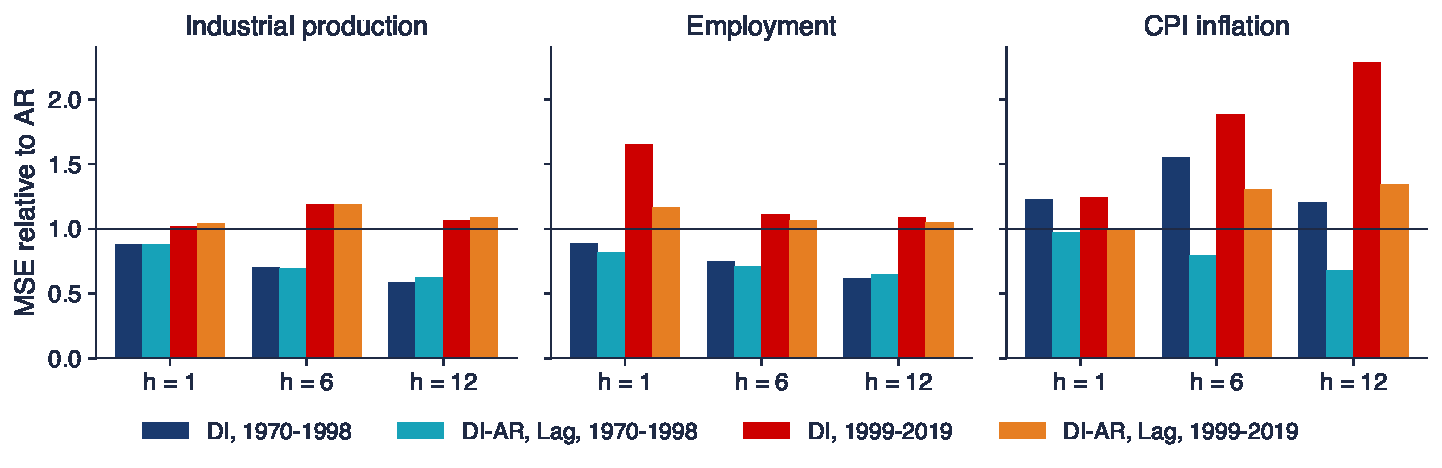
\includegraphics[width=0.97\textwidth,height=0.5\textheight,keepaspectratio]{ats_ch5_di.pdf}
\end{center}
\vspace{-0.25cm}
\begin{itemize}
    \item MSE relativ la prognoza AR cu decalaje alese prin BIC (sub 1 = mai bine)
\end{itemize}
\quantlet{ATS\_ch5\_factors}{\qlurl{ATS_ch5_factors}}
\end{frame}

\begin{frame}{Interpretarea indicilor de difuziune}
\itemsize{\small}
\begin{itemize}
    \item 1970--1998: cîștiguri mari pentru activitatea reală la $h = 12$: IP 0{,}58, ocupare 0{,}62; pentru inflație doar cu decalajele proprii (DI-AR, Lag 0{,}68)
    \item 1999--2019: cîștigurile dispar (IP 1{,}07, ocupare 1{,}09, inflație 1{,}35): Marea Moderație a făcut activitatea mai puțin previzibilă din panel
    \item BIC alege în mediană 7 factori (10\%--90\%: 5--12) pentru DI-AR, Lag la $h = 12$
    \item Shrinkage-ul bayesian și componentele principale dau prognoze puternic corelate în panelurile mari \refDGRa: două căi pentru aceeași informație
\end{itemize}
\end{frame}

\begin{frame}{Recapitulare: modele factoriale}
\itemsize{\small}
\begin{itemize}
    \item Cîțiva factori rezumă o sută de serii; PCA estimează consistent spațiul factorilor cînd $N, T \to \infty$
    \item Criteriile Bai--Ng aleg numărul de factori; verificați sensibilitatea lor
    \item Indicii de difuziune au ajutat mult înainte de 1999 și mult mai puțin după: evaluați pe mai multe perioade
\end{itemize}
\end{frame}


%=============================================================================
\section{Modele VAR augmentate cu factori}
%=============================================================================

\begin{frame}{FAVAR: Bernanke, Boivin și Eliasz (2005)}
\itemsize{\footnotesize}
\begin{columns}[T]
\begin{column}{0.30\textwidth}
\centering

\includegraphics[height=0.32\textheight]{ch5_bernanke_2008.jpg}\\[1mm]
\imgcap{Ben Bernanke, 2008}
\imgcredit{https://commons.wikimedia.org/wiki/File:Ben_Bernanke_official_portrait_(cropped).jpg}{Foto: Federal Reserve (2008); domeniu public; Wikimedia Commons}
\end{column}
\begin{column}{0.68\textwidth}
\begin{itemize}
    \item \refBBE: $\binom{F_t}{Y_t} = \Phi(L)\binom{F_{t-1}}{Y_{t-1}} + v_t$, $X_t = \Lambda^fF_t + \Lambda^yY_t + e_t$, $Y_t$ = dobînda federal funds
    \begin{itemize}
        \item VAR-ul vede informația a 100 de serii prin $K$ factori; răspunsurile sînt disponibile pentru fiecare serie din $X_t$
    \end{itemize}
    \item Estimarea în doi pași (secțiunea III): componentele principale $\hat C_t$ ale lui $X_t$; factorii lenți din seriile lente; eliminăm $Y_t$: $\hat F_t = \hat C_t - \hat b_Y Y_t$
    \begin{itemize}
        \item $K = 3$, VAR(13), 1960:1--2001:8 (la noi: $T = 500$, $N = 102$ serii complete, 76 lente); Cholesky cu $Y_t$ ultimul; șoc de 25 bp
    \end{itemize}
    \item Prețurile și masa monetară intră ca rate lunare de creștere; răspunsurile se cumulează în niveluri
\end{itemize}
\end{column}
\end{columns}
\end{frame}

\begin{frame}{Răspunsurile FAVAR la un șoc de politică monetară de 25 bp}
\itemsize{\footnotesize}
\begin{center}
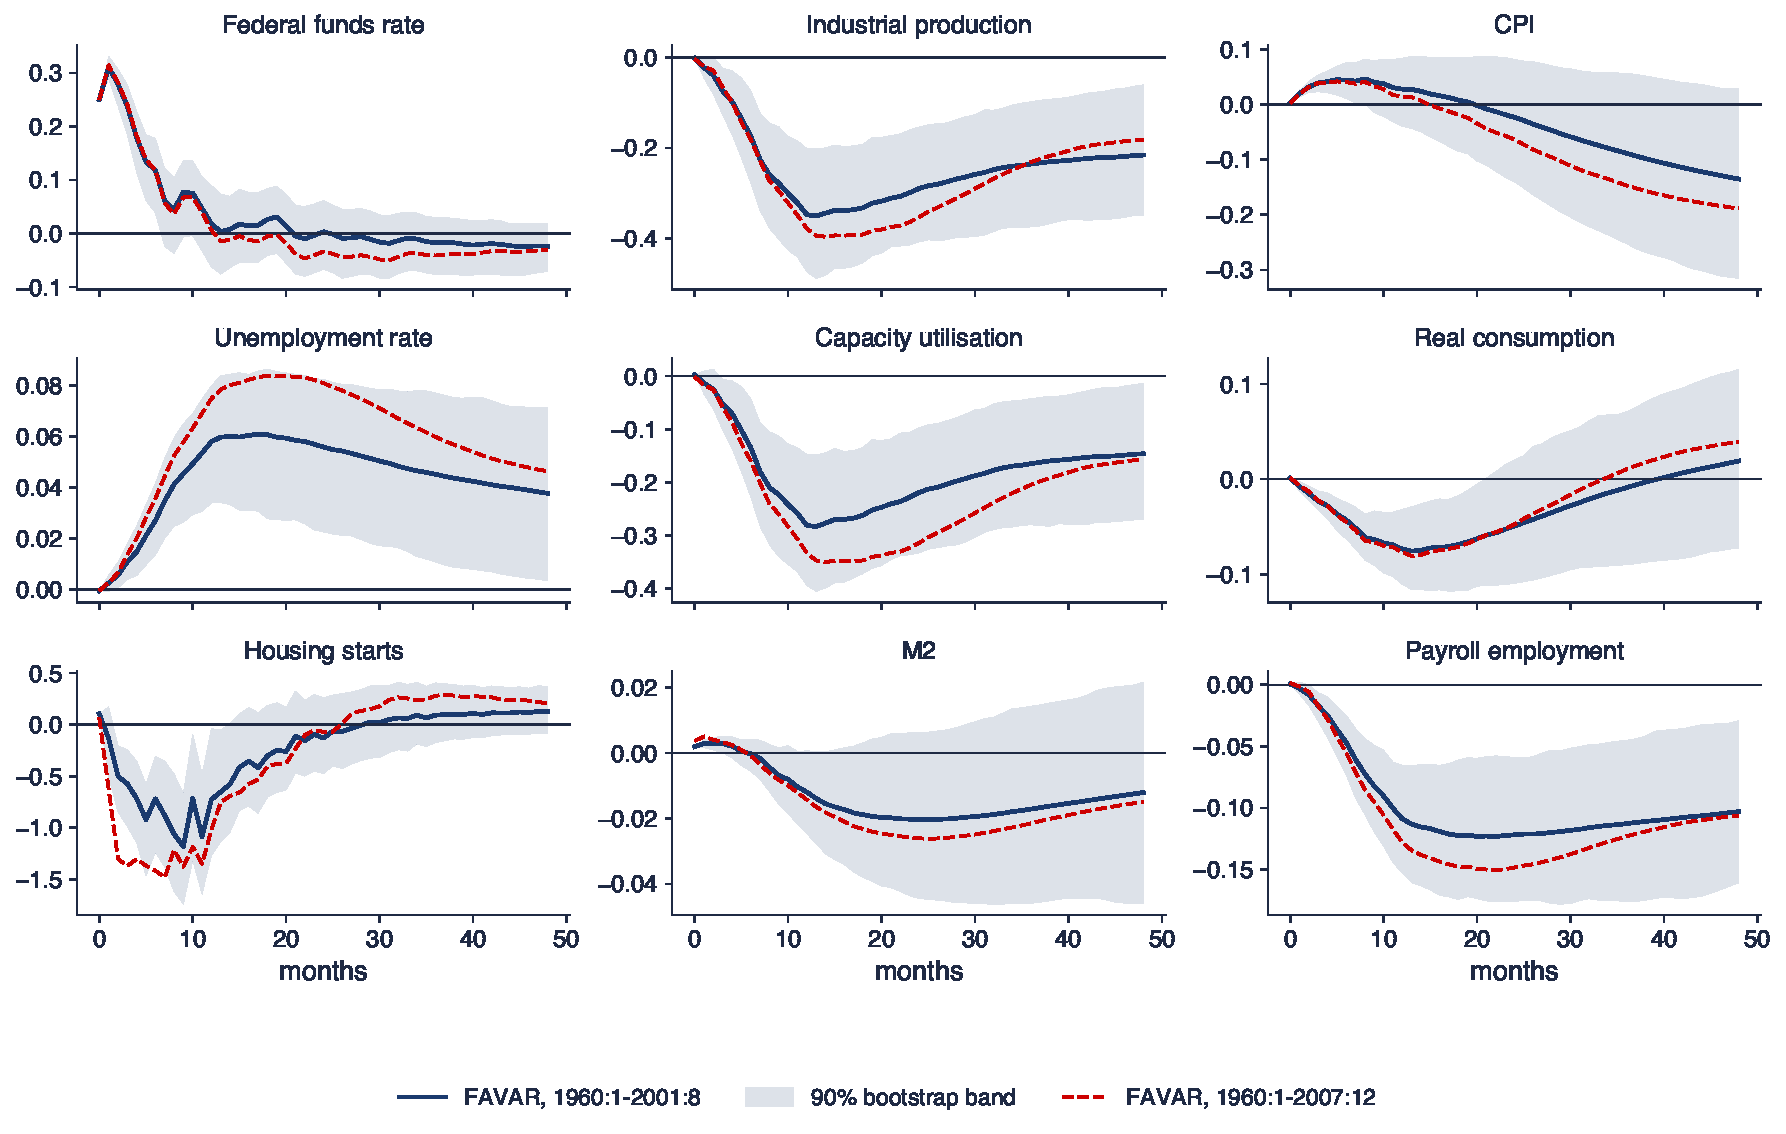
\includegraphics[width=0.97\textwidth,height=0.6\textheight,keepaspectratio]{ats_ch5_favar.pdf}
\end{center}
\vspace{-0.25cm}
\begin{itemize}
    \item Niveluri în procente (dobînzi și șomaj în pp); benzi bootstrap pe reziduuri de 90\%, factorii tratați ca date; linia întreruptă: eșantion pînă în 2007:12
\end{itemize}
\quantlet{ATS\_ch5\_favar}{\qlurl{ATS_ch5_favar}}
\end{frame}

\begin{frame}{Interpretarea FAVAR}
\itemsize{\small}
\begin{itemize}
    \item Activitatea reală scade cu întîrziere: IP minim \ensuremath{-}0{,}35\% după 13 luni, gradul de utilizare a capacităților \ensuremath{-}0{,}28 pp, numărul de salariați \ensuremath{-}0{,}12\%, șomajul crește cu 0{,}061 pp
    \item Locuințele începute reacționează primele și cel mai puternic (\ensuremath{-}1{,}18\% după 9 luni): sectorul sensibil la dobîndă
    \item Anomalia prețurilor este mică (cel mult 0{,}046\%, luna 8); IPC ajunge la \ensuremath{-}0{,}14\% după 48 de luni (banda [\ensuremath{-}0{,}32; 0{,}03]); pînă în 2007: \ensuremath{-}0{,}19\%
    \item Seminarul 5, B4: cu $K = 1$ sau $K = 5$ anomalia revine; alegerea lui $K$ este o ipoteză de identificare, nu un detaliu
\end{itemize}
\end{frame}


%=============================================================================
\section{Modele factoriale dinamice în forma spațiului stărilor}
%=============================================================================

\begin{frame}{Modelul factorial dinamic}
\itemsize{\small}
\begin{itemize}
    \item Ecuația de măsurare: $x_t = \Lambda f_t + e_t$, $e_t \sim N(0, \Psi)$, $\Psi$ diagonală; ecuația de tranziție: $f_t = A_1f_{t-1} + \dots + A_qf_{t-q} + u_t$, $u_t \sim N(0, Q)$
    \begin{itemize}
        \item un model în spațiul stărilor (\atschlink{https://danpele.github.io/Time-Series-Analysis/RO/Cursuri/capitol10_spatiul_starilor_kalman_markov_switching.pdf}{TSA, Capitolul 10}; \atschlink{https://danpele.github.io/Advanced-Time-Series/RO/Cursuri/capitol6_modele_spatiul_starilor_filtrare_bayesiana.pdf}{Capitolul 6}): starea $s_t = (f_t', \dots, f_{t-m}')'$, filtrul și netezitorul Kalman
    \end{itemize}
    \item \textbf{În doi pași} \refDGRb: PCA pentru $\hat f_t$, OLS pentru $\Lambda$ și $\Psi$, un VAR pe $\hat f_t$ pentru $A$ și $Q$, apoi netezitorul Kalman reestimează $f_t$
    \begin{itemize}
        \item consistent pentru $N$ și $T$ mari, deși $\Psi$ diagonală este o specificare greșită
    \end{itemize}
    \item \textbf{Verosimilitate cvasi-maximă prin EM} \refDGRc, \refBM: pasul E = netezitorul Kalman, pasul M = regresii pe momentele netezite; tratează orice structură de date lipsă și componente idiosincratice AR(1)
\end{itemize}
\end{frame}

\begin{frame}{Datele lipsă nu sînt o problemă pentru filtrul Kalman}
\itemsize{\small}
\begin{itemize}
    \item La momentul $t$ păstrăm doar liniile observate: $x_t^o = W_tx_t$, $\Lambda_t = W_t\Lambda$, $\Psi_t = W_t\Psi W_t'$, cu $W_t$ o matrice de selecție
    \begin{itemize}
        \item dacă nu se observă nimic, pasul de actualizare se omite și predicția se transmite mai departe
    \end{itemize}
    \item \textbf{Date incomplete la sfîrșitul eșantionului (ragged edge)}: fiecare serie se oprește în altă lună (întîrzieri de publicare); filtrul folosește ce există
    \begin{itemize}
        \item același mecanism tratează seriile care încep tîrziu (încrederea în servicii din 2002) și seriile trimestriale observate în fiecare a treia lună
    \end{itemize}
    \item De aceea nowcasting-ul este o problemă de filtrare și de aceea \atschlink{https://danpele.github.io/Advanced-Time-Series/RO/Cursuri/capitol6_modele_spatiul_starilor_filtrare_bayesiana.pdf}{Capitolul 6} dezvoltă filtrul complet
\end{itemize}
\end{frame}


%=============================================================================
\section{Frecvențe mixte și nowcasting}
%=============================================================================

\begin{frame}{Problema nowcasting-ului}
\itemsize{\footnotesize}
\begin{columns}[T]
\begin{column}{0.32\textwidth}
\centering
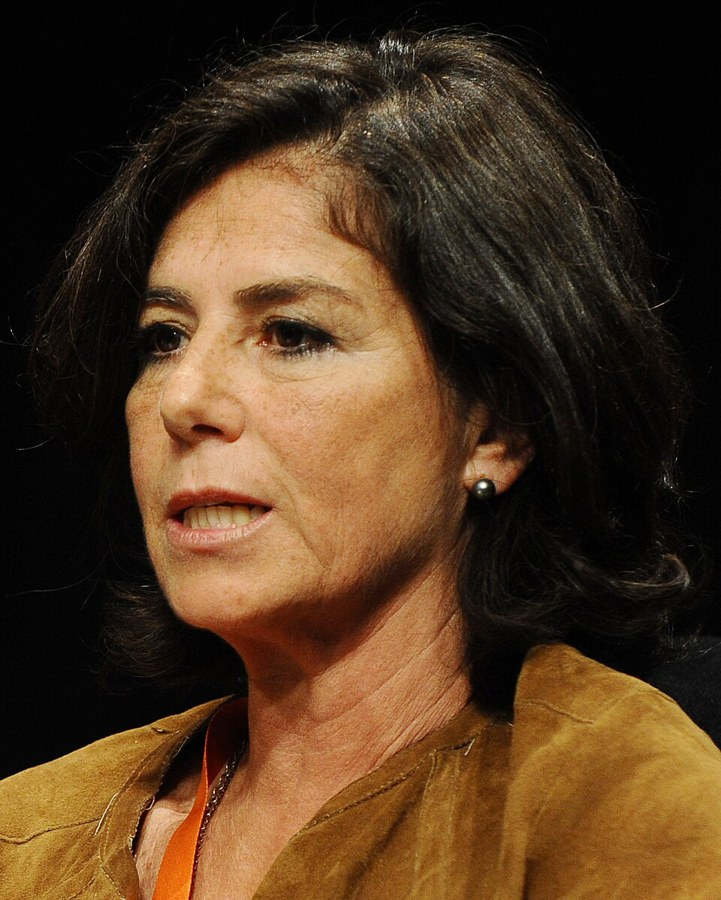
\includegraphics[height=0.34\textheight]{ch5_reichlin_2013.jpg}\\[1mm]
\imgcap{Lucrezia Reichlin, 2013}
\imgcredit{https://commons.wikimedia.org/wiki/File:Lucrezia_Reichlin_-_Festival_Economia_2013_(cropped).JPG}{Foto: Niccolò Caranti (2013); CC BY-SA 3.0; Wikimedia Commons}
\end{column}
\begin{column}{0.66\textwidth}
\begin{itemize}
    \item \textbf{Nowcasting}: estimarea prezentului și a trecutului recent al unei variabile de frecvență joasă (PIB) din date de frecvență înaltă, publicate mai repede \refGRS, \refBGMR
    \begin{itemize}
        \item backcast (trimestrul trecut, încă nepublicat), nowcast (trimestrul curent), forecast (trimestrul următor)
    \end{itemize}
    \item Trei dificultăți: frecvențe mixte, mulți indicatori, publicări asincrone (ragged edge)
    \begin{itemize}
        \item anchetele apar la sfîrșitul lunii; producția industrială după mai mult de o lună; PIB-ul la cîteva săptămîni după trimestru
    \end{itemize}
    \item Instrumente: ecuații punte \refBGP, MIDAS \refGSV, \refGSVb, DFM cu frecvențe mixte \refMM, \refBM{} și VAR cu frecvențe mixte \refSS
\end{itemize}
\end{column}
\end{columns}
\end{frame}

\begin{frame}{Ecuații punte și MIDAS}
\itemsize{\small}
\begin{itemize}
    \item \textbf{Punte}: prognozăm lunile lipsă ale fiecărui indicator (AR), agregăm la trimestru, regresăm PIB-ul pe agregatele trimestriale \refBGP
    \begin{itemize}
        \item simplă și transparentă; eroarea prognozelor AR lunare trece în nowcast
    \end{itemize}
    \item \textbf{MIDAS} \refGSV: $y_\tau = \beta_0 + \beta_1\sum_{j=0}^{K-1}w_j(\theta)x_{m_\tau - j} + \rho y_{\tau - s} + \varepsilon_\tau$, cu ultima valoare lunară disponibilă $x_{m_\tau}$
    \begin{itemize}
        \item Almon exponențial: $w_j(\theta) = e^{\theta_1j + \theta_2j^2}/\sum_ke^{\theta_1k + \theta_2k^2}$; doi parametri pentru $K$ decalaje, estimați prin NLS
        \item MIDAS cu valori anticipate \refAGK, \refCG: o regresie pentru fiecare set de informații; U-MIDAS lasă $w_j$ nerestricționate cînd $K$ este mic \refFMS
    \end{itemize}
    \item Niciuna nu folosește dinamica comună a indicatorilor; DFM o folosește
\end{itemize}
\end{frame}

\begin{frame}{Legătura dintre luni și trimestre: Mariano și Murasawa (2003)}
\itemsize{\small}
\begin{itemize}
    \item Fie $Y_t^M$ un nivel lunar latent, iar PIB-ul trimestrial media pe 3 luni, observată în a treia lună
    \begin{itemize}
        \item aproximarea prin media geometrică: $\ln Y_t^Q \approx \frac13(\ln Y_t^M + \ln Y_{t-1}^M + \ln Y_{t-2}^M)$
        \item creșterea trimestrială $y_t^Q = \ln Y_t^Q - \ln Y_{t-3}^Q = \frac13(y_t + 2y_{t-1} + 3y_{t-2} + 2y_{t-3} + y_{t-4})$, $y_t$ = creșterea lunară \refMM
    \end{itemize}
    \item În DFM: $y_t^Q = \lambda_y'\sum_{j=0}^{4}w_jf_{t-j} + e_t^Q$, $w = (1, 2, 3, 2, 1)/3$: starea trebuie să conțină cinci decalaje ale lui $f_t$
    \begin{itemize}
        \item PIB-ul este o variabilă lunară observată din trei în trei luni: lipsește în lunile 1 și 2 ale fiecărui trimestru
    \end{itemize}
    \item Seminarul 5, A7: ponderile de mînă
\end{itemize}
\end{frame}

\begin{frame}{Studiu de caz: nowcasting pentru PIB-ul României}
\itemsize{\footnotesize}
\begin{columns}[T]
\begin{column}{0.34\textwidth}
\centering
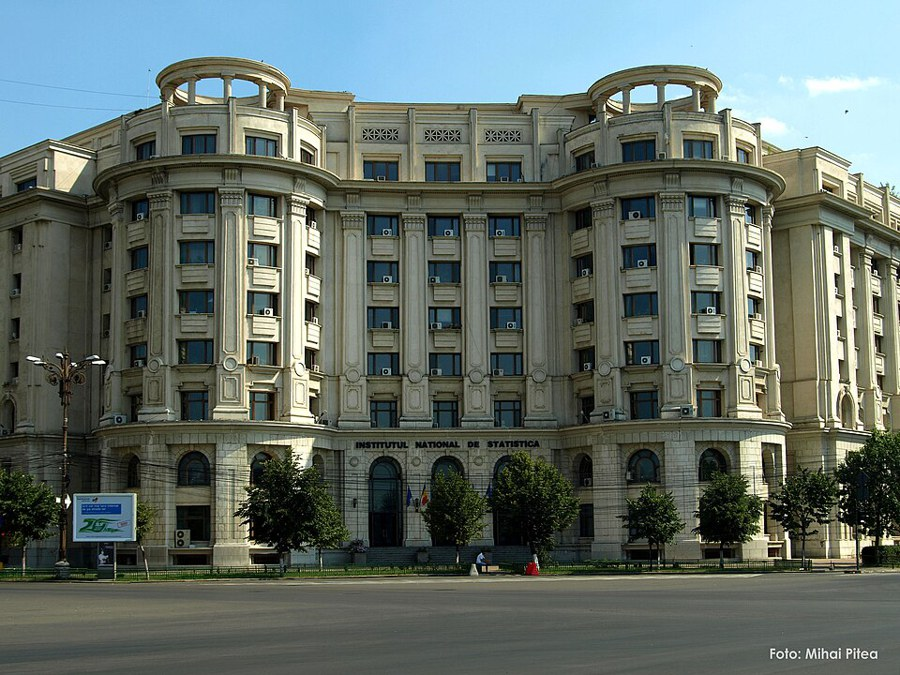
\includegraphics[height=0.3\textheight]{ch5_ins_bucharest_2009.jpg}\\[1mm]
\imgcap{Institutul Național de Statistică, București}
\imgcredit{https://commons.wikimedia.org/wiki/File:Institutul_Național_de_Statistică.jpg}{Foto: Dan Mihai Pitea (2009); CC BY-SA 3.0; Wikimedia Commons}
\end{column}
\begin{column}{0.64\textwidth}
\begin{itemize}
    \item Ținta: creșterea t/t a PIB-ului real (Eurostat), 94 de trimestre pînă în T2 2026; panelul lunar: 11 serii din 2003 (Eurostat)
    \begin{itemize}
        \item date „hard” ca rate lunare de creștere: IP, comerț, construcții, IP din zona euro; variația șomajului; nivelurile a șase solduri de încredere
    \end{itemize}
    \item Întîrzieri stilizate de publicare la sfîrșitul fiecărei luni: anchete 0, șomaj 1, date hard 2 luni; PIB-ul la 2 luni după trimestru
    \begin{itemize}
        \item datele din ediția curentă: pseudo timp real (fără revizuiri)
    \end{itemize}
    \item Modelele: AR(1), punte (IP, comerț, ESI), MIDAS (IP, ESI; $K = 6$), DFM cu doi factori (în doi pași și EM)
\end{itemize}
\end{column}
\end{columns}
\end{frame}

\begin{frame}{PIB-ul României și doi indicatori lunari}
\itemsize{\footnotesize}
\begin{center}
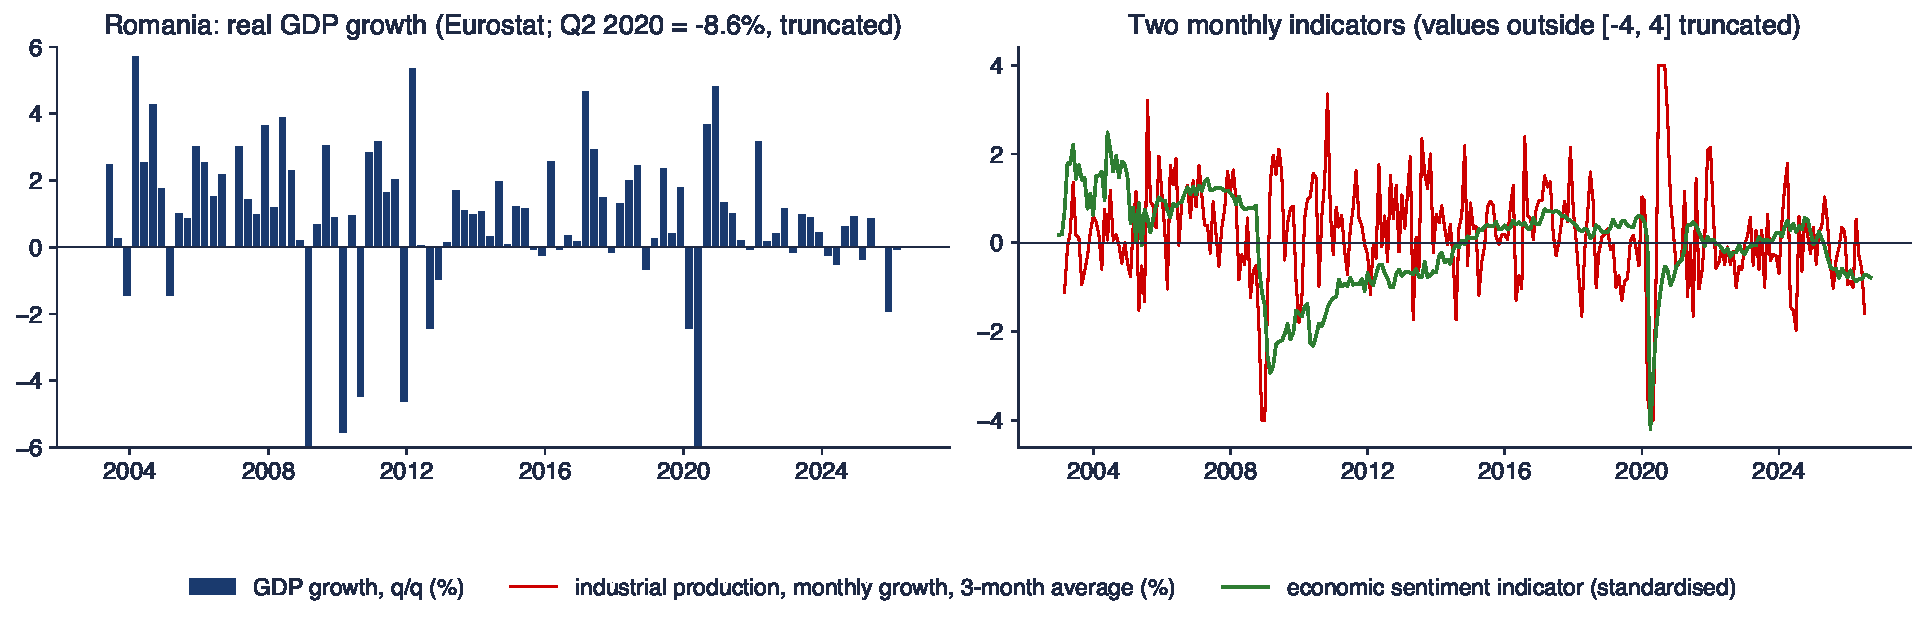
\includegraphics[width=0.97\textwidth,height=0.5\textheight,keepaspectratio]{ats_ch5_ro_data.pdf}
\end{center}
\vspace{-0.25cm}
\begin{itemize}
    \item Creșterea trimestrială a PIB-ului (T2 2020: \ensuremath{-}8{,}6\%, trunchiată); creșterea IP (medie pe 3 luni) și ESI standardizat
\end{itemize}
\quantlet{ATS\_ch5\_nowcast}{\qlurl{ATS_ch5_nowcast}}
\end{frame}

\begin{frame}{Interpretarea datelor pentru România}
\itemsize{\small}
\begin{itemize}
    \item Creșterea trimestrială este volatilă: oscilațiile de $\pm 5$ pp din 2009--2012 și prăbușirea din 2020 domină varianța
    \item ESI (medie pe 3 luni) are corelația 0{,}44 cu creșterea PIB înainte de 2020: informativ, departe de perfect
    \item Ultimul trimestru publicat: T2 2026, creștere 0{,}00\%; ținta nowcast-ului este T3 2026
\end{itemize}
\end{frame}

\begin{frame}{Ponderile MIDAS pentru România}
\itemsize{\footnotesize}
\begin{center}
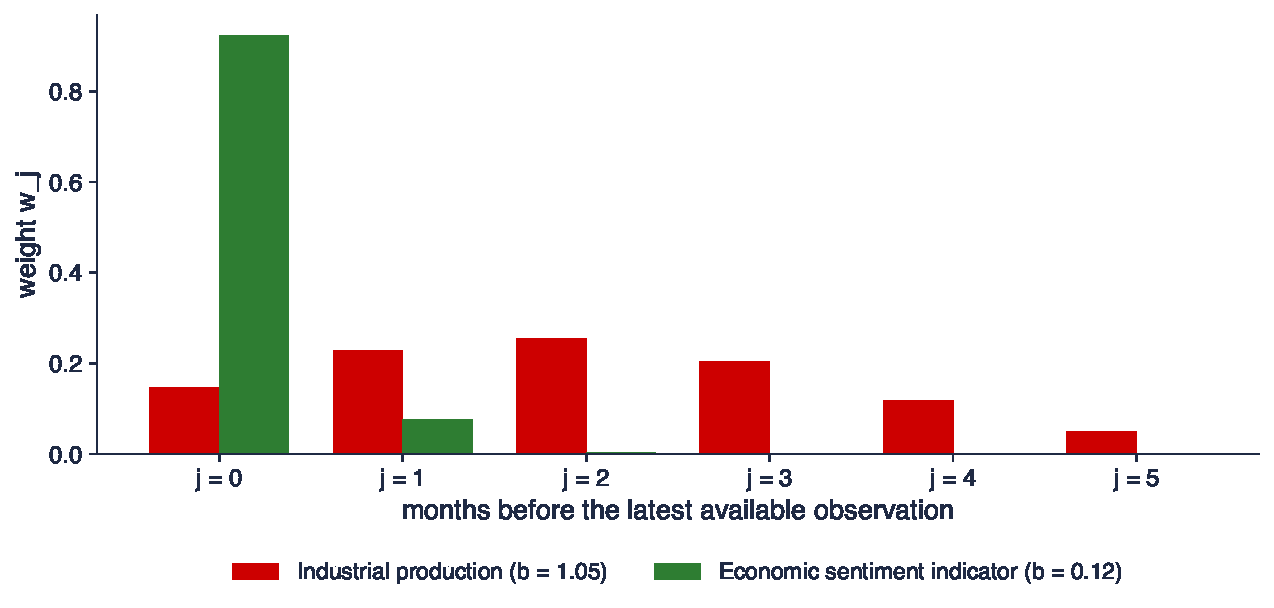
\includegraphics[width=0.97\textwidth,height=0.48\textheight,keepaspectratio]{ats_ch5_midas.pdf}
\end{center}
\vspace{-0.25cm}
\begin{itemize}
    \item ADL-MIDAS cu ponderi Almon exponențiale la sfîrșitul lunii a treia a trimestrului, 2003--2026
\end{itemize}
\quantlet{ATS\_ch5\_nowcast}{\qlurl{ATS_ch5_nowcast}}
\end{frame}

\begin{frame}{Interpretarea ponderilor MIDAS}
\itemsize{\small}
\begin{itemize}
    \item IP: ponderi în formă de cocoașă, cu maximul la decalajul 2 (0{,}25): contează lunile trimestrului însuși, cum prezic ponderile Mariano--Murasawa
    \item ESI: ponderea 0{,}92 pe ultima lună: un indicator de nivel rezumă deja trecutul
    \item Creșterea PIB decalată are coeficientul \ensuremath{-}0{,}28: seria zgomotoasă t/t revine la medie
\end{itemize}
\end{frame}

\begin{frame}{Evaluarea în pseudo timp real}
\itemsize{\small}
\begin{itemize}
    \item Pentru fiecare trimestru T1 2013--T2 2026, nowcast-uri la sfîrșitul lunilor 1, 2, 3 ale trimestrului și la sfîrșitul primei luni de după
    \begin{itemize}
        \item toți parametrii sînt reestimați pe datele disponibile la acea dată; T2--T3 2020 sînt excluse din RMSE (raportăm și cu ele)
    \end{itemize}
    \item Eșantionul de evaluare începe în 2013 pentru că oscilațiile din 2009--2012 sînt mai mari decît orice eroare de model; din 2010 RMSE urcă la aproximativ 2 pp pentru toate modelele
    \begin{itemize}
        \item abaterea standard a țintei 2013--2026 (fără T2--T3 2020): 1{,}33 pp
    \end{itemize}
    \item Întrebarea: scade RMSE pe măsură ce trimestrul avansează și cu cît față de un AR?
\end{itemize}
\end{frame}

\begin{frame}{Acuratețea nowcast-ului în funcție de setul de informații}
\itemsize{\footnotesize}
\begin{center}
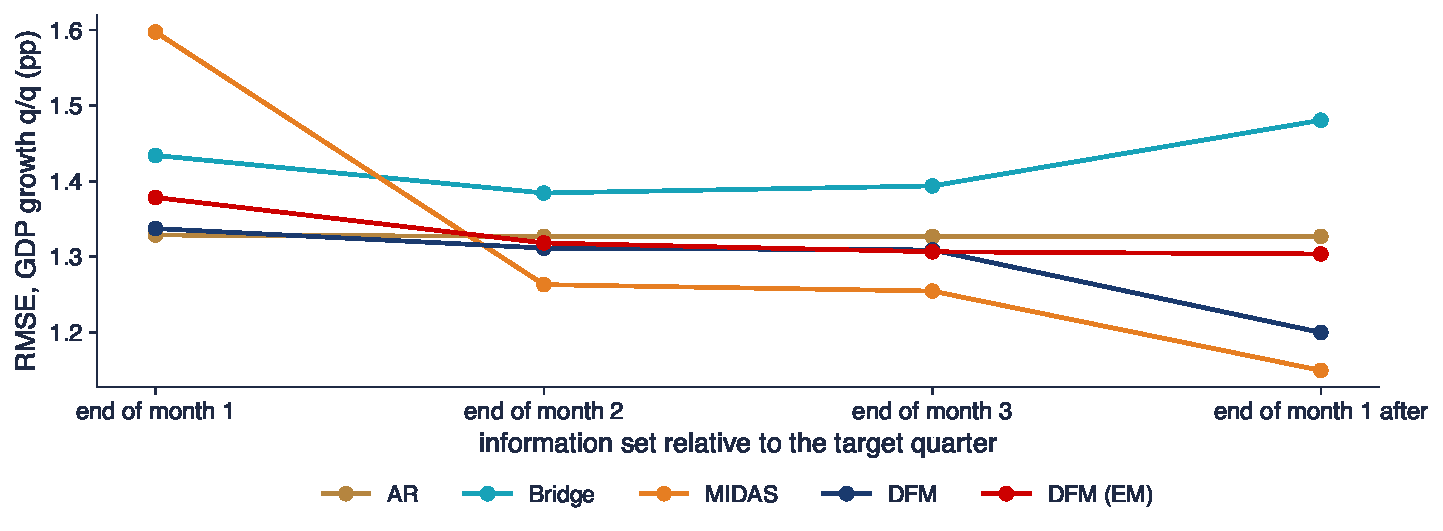
\includegraphics[width=0.97\textwidth,height=0.5\textheight,keepaspectratio]{ats_ch5_nowcast.pdf}
\end{center}
\vspace{-0.25cm}
\begin{itemize}
    \item RMSE al nowcast-urilor pentru creșterea t/t a PIB-ului, T1 2013--T2 2026 fără T2--T3 2020
\end{itemize}
\quantlet{ATS\_ch5\_nowcast}{\qlurl{ATS_ch5_nowcast}}
\end{frame}

\begin{frame}{Interpretarea acurateței nowcast-ului}
\itemsize{\small}
\begin{itemize}
    \item AR: 1{,}33 pp peste tot; DFM: de la 1{,}34 (luna 1) la 1{,}20 (luna 1 de după); MIDAS: de la 1{,}60 la 1{,}15
    \item Ecuația punte nu bate AR (1{,}39); estimarea EM a DFM este apropiată de AR (1{,}31 în luna 3)
    \item Diebold--Mariano DFM comparat cu AR în luna 3: $t = \ensuremath{-}0{,}30$, $p = 0{,}76$: cîștigul nu este semnificativ pe 54 de trimestre
    \item Cu 2020: AR 1{,}90, DFM 1{,}30 în luna 1 de după: datele lunare surprind prăbușirea, AR nu poate
\end{itemize}
\end{frame}

\begin{frame}{Știri și revizuiri: Bańbura și Modugno (2014)}
\itemsize{\small}
\begin{itemize}
    \item Seturile de informații $\Omega_v \subset \Omega_{v+1}$; noile publicări $x_j$, $j \in J_{v+1}$; \textbf{știrea} este $I_j = x_j - \E[x_j\mid\Omega_v]$, nu $x_j$
    \begin{itemize}
        \item cu parametri ficși: $\E[y\mid\Omega_{v+1}] - \E[y\mid\Omega_v] = \E[yI']\E[II']^{-1}I = \sum_j w_jI_j$ \refBM
    \end{itemize}
    \item În DFM: $I_j = \lambda_j'(f_{t_j} - \hat f_{t_j\mid v}) + e_j$, deci $\E[II'] = H P_{\mid v}H' + \Psi_J$ și $\E[yI'] = z_y'P_{\mid v}H'$
    \begin{itemize}
        \item $P_{\mid v}$: covarianța stării stivuite dat fiind $\Omega_v$, din filtrul Kalman
    \end{itemize}
    \item O publicare mare dar așteptată nu schimbă nimic; o surpriză mică într-o serie cu pondere mare schimbă mult; publicările corelate își împart ponderea
\end{itemize}
\end{frame}

\begin{frame}{Nowcast pentru T3 2026 și sursa revizuirii}
\itemsize{\footnotesize}
\begin{center}
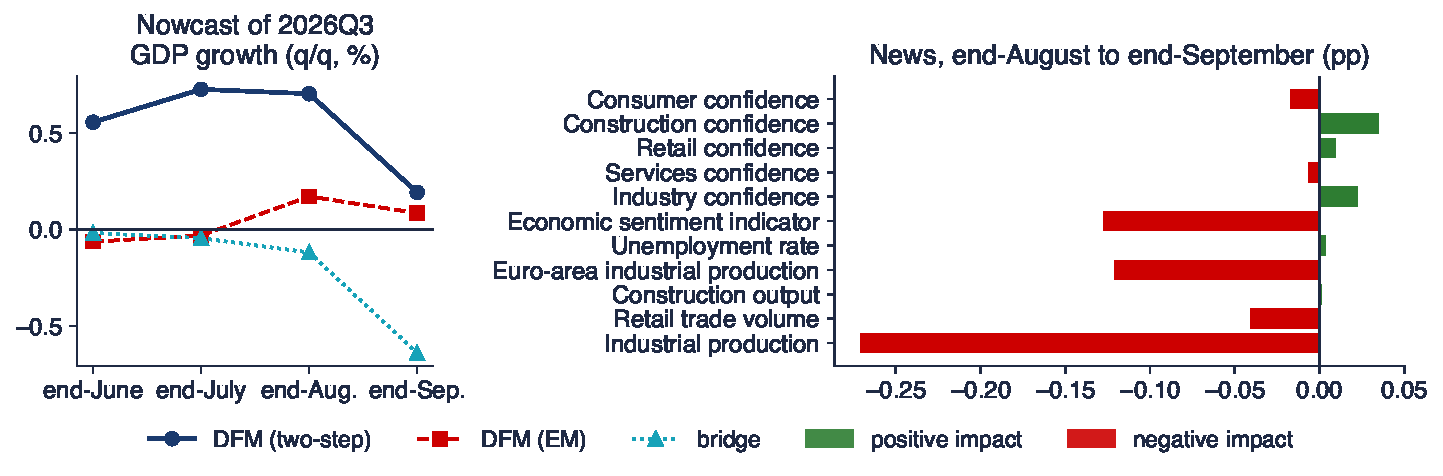
\includegraphics[width=0.97\textwidth,height=0.5\textheight,keepaspectratio]{ats_ch5_news.pdf}
\end{center}
\vspace{-0.25cm}
\begin{itemize}
    \item Stînga: nowcast-uri la sfîrșitul lunilor iunie--septembrie 2026; dreapta: descompunerea în știri a nowcast-ului DFM în doi pași între seturile de informații din august și septembrie
\end{itemize}
\quantlet{ATS\_ch5\_nowcast}{\qlurl{ATS_ch5_nowcast}}
\end{frame}

\begin{frame}{Interpretarea știrilor}
\itemsize{\small}
\begin{itemize}
    \item Nowcast-ul DFM pentru T3 2026: 0{,}70\% la sfîrșitul lui august, 0{,}19\% la sfîrșitul lui septembrie; cele 11 publicări noi însumează exact \ensuremath{-}0{,}51 pp
    \item Publicarea IP pentru iulie a fost cu \ensuremath{-}3{,}7 pp sub așteptarea modelului; cu ponderea 0{,}073 a redus nowcast-ul cu \ensuremath{-}0{,}27 pp; ESI \ensuremath{-}0{,}13, IP din zona euro \ensuremath{-}0{,}12
    \item Alte modele la sfîrșitul lui septembrie: DFM EM 0{,}08\%, punte \ensuremath{-}0{,}64\%, AR 0{,}76\%: prima estimare oficială pentru T3 2026 le va judeca
    \item Descompunerea în știri transformă o cifră într-o explicație pe care o bancă centrală o poate verifica publicare cu publicare
\end{itemize}
\end{frame}

\begin{frame}{Recapitulare: nowcasting}
\itemsize{\small}
\begin{itemize}
    \item Nowcasting = filtrarea unui sistem cu frecvențe mixte și date incomplete la sfîrșitul eșantionului
    \item Ecuațiile punte, MIDAS și DFM folosesc aceeași legătură Mariano--Murasawa între luni și trimestre
    \item Pentru România, datele lunare îmbunătățesc nowcast-ul spre sfîrșitul trimestrului; cîștigul este modest și nesemnificativ
    \item Orice revizuire se descompune exact în știri cînd parametrii sînt ficși
\end{itemize}
\end{frame}


%=============================================================================
\section{AI în descoperirea științifică}
%=============================================================================

\begin{frame}{O întrebare deschisă}
\itemsize{\small}
\begin{itemize}
    \item Poate un model de nowcasting să bată în mod semnificativ statistic un AR simplu pentru creșterea PIB-ului României și ce publicări poartă informația?
    \begin{itemize}
        \item formal: $H_0$: MSE egal pentru nowcast-urile DFM și AR la sfîrșitul lunii 3 (Diebold--Mariano, \atschlink{https://danpele.github.io/Advanced-Time-Series/RO/Cursuri/capitol1_evaluarea_prognozelor.pdf}{Capitolul 1}), cu eșantionul, modelele și decalajele preînregistrate
        \item infirmată de o respingere pe trimestre pe care modelul nu le-a văzut, cu ediții în timp real ale PIB
    \end{itemize}
    \item De ce contează: deciziile fiscale și monetare din 2025--2026 s-au luat cu PIB-ul cunoscut la cîteva săptămîni după fiecare trimestru
    \begin{itemize}
        \item literatura de pornire: \refGRS, \refBM, \refBGMR, \refGLPb, \refSS
    \end{itemize}
\end{itemize}
\end{frame}

\begin{frame}{Bucla de cercetare cu un asistent AI}
\itemsize{\footnotesize}
\begin{itemize}
    \item Un asistent AI (un LLM precum Claude, ChatGPT, Gemini sau Copilot) accelerează fiecare etapă; Semantic Scholar și Elicit ajută la literatură
    \begin{itemize}
        \item \textbf{literatura}: \aiprompt{Listează articole recenzate care fac nowcasting pentru PIB-ul țărilor din Europa Centrală și de Est cu modele factoriale sau MIDAS; dă DOI-urile.} Apoi verificați fiecare DOI pe Crossref
        \item \textbf{ipoteza}: \aiprompt{Ce publicări lunare din România ar trebui să conțină știri despre PIB și în ce lună a trimestrului?}
        \item \textbf{cod și replicare}: cereți un filtru Kalman cu date lipsă, apoi reproduceți întîi o cifră cunoscută (suma știrilor din acest curs)
        \item \textbf{robustețe și critică}: \aiprompt{Joacă rolul unui recenzent ostil al unui articol de nowcasting: enumeră felurile în care designul în pseudo timp real ar putea avantaja modelul.}
    \end{itemize}
    \item Raportul: ce s-a cerut, ce s-a păstrat, ce s-a respins (AI\_USE.md, AI\_ERRORS.md)
\end{itemize}
\end{frame}

\begin{frame}{Verificări necesare}
\itemsize{\small}
\begin{itemize}
    \item Fiecare referință există și spune ce se afirmă (DOI-ul funcționează, titlul coincide, rezultatul se află în lucrare)
    \item Setul de informații la fiecare dată conține doar datele publicate pînă atunci; datele din ediția curentă supraestimează acuratețea
    \item Hiperparametrii, factorii și decalajele se aleg în interiorul fiecărei ferestre de estimare, niciodată pe eșantionul de evaluare
    \item Perioada de evaluare și tratarea anului 2020 sînt fixate înaintea rezultatelor; toate variantele sînt raportate
    \item O afirmație despre „nowcast-uri mai bune” se sprijină pe un test, nu doar pe un RMSE mai mic
\end{itemize}
\end{frame}

\begin{frame}{Mini studiu de caz: cît de robustă este o clasificare?}
\itemsize{\footnotesize}
\begin{center}
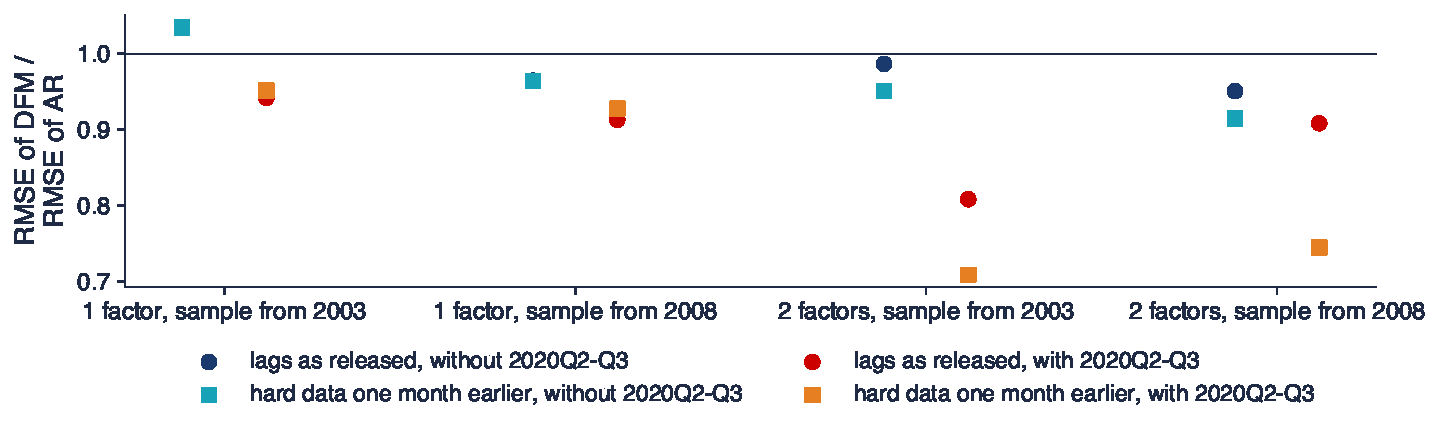
\includegraphics[width=0.97\textwidth,height=0.48\textheight,keepaspectratio]{ats_ch5_ai_case.pdf}
\end{center}
\vspace{-0.25cm}
\begin{itemize}
    \item RMSE al nowcast-ului DFM relativ la AR la sfîrșitul lunii 3, 2013--2026, pentru diferite numere de factori, începuturi ale eșantionului, întîrzieri de publicare și tratări ale anului 2020
    \item Cele 16 variante variază între 0{,}71 și 1{,}03; DFM cîștigă în 14 dintre ele: un rezumat AI care raportează cea mai bună variantă drept „rezultatul” greșește
\end{itemize}
\quantlet{ATS\_ch5\_nowcast}{\qlurl{ATS_ch5_nowcast}}
\end{frame}

\begin{frame}{Idee de proiect}
\itemsize{\small}
\begin{itemize}
    \item \textbf{Un model de nowcasting în timp real pentru PIB-ul României}: întîi replicare, apoi extindere
    \begin{itemize}
        \item replicați: descompunerea în știri din acest curs (\ensuremath{-}0{,}51 pp între august și septembrie 2026) și tabelul BGR pentru 1971--2003
        \item extindeți: datele reale de publicare (calendarul INS), edițiile PIB salvate de acum înainte, blocuri de factori pentru date hard și soft, un BVAR cu frecvențe mixte, nowcast-uri de densitate
        \item preînregistrați: ținta, trimestrele, modelele, seturile de informații, tratarea anului 2020 și testul Diebold--Mariano
    \end{itemize}
    \item Livrabilele urmează regulile cursului: repository, raport, AI\_USE.md, AI\_ERRORS.md, susținere orală
\end{itemize}
\end{frame}


%=============================================================================
\section{Încheiere}
%=============================================================================

\begin{frame}{Idei de reținut}
\itemsize{\small}
\begin{itemize}
    \item Multe serii și puține observații: strîngeți (distribuții a priori) sau comprimați (factori)
    \item Distribuția Minnesota în formă conjugată dă distribuții a posteriori închise, extrageri exacte și o verosimilitate marginală care alege shrinkage-ul
    \item Sistemele mai mari cer distribuții mai strînse; atunci prognozează mai bine și dau răspunsuri mai plauzibile
    \item Componentele principale estimează spațiul factorilor; Bai--Ng îi alege dimensiunea; FAVAR și DFM îl folosesc
    \item Nowcasting-ul este filtrare Kalman cu date incomplete la sfîrșitul eșantionului; orice revizuire este o sumă de știri
\end{itemize}
\end{frame}

\begin{frame}{Autoevaluare}
\itemsize{\small}
\begin{columns}[T]
\begin{column}{0.56\textwidth}
\begin{block}{Întrebări}
\begin{itemize}
    \item Ce se întîmplă cu media a posteriori Minnesota cînd $\lambda \to 0$?
    \item De ce impune distribuția natural conjugată $\vartheta = 1$?
    \item Ce distribuție permite cointegrarea: suma coeficienților sau observația inițială?
    \item De ce poate identifica PCA doar spațiul factorilor?
    \item De ce o publicare mare, dar așteptată, nu este o știre?
\end{itemize}
\end{block}
\end{column}
\begin{column}{0.40\textwidth}
\begin{block}{Urmează: \atschlink{https://danpele.github.io/Advanced-Time-Series/RO/Cursuri/capitol6_modele_spatiul_starilor_filtrare_bayesiana.pdf}{Capitolul 6}}
\begin{itemize}
    \item Modele în spațiul stărilor și filtrare bayesiană
    \item Filtrul și netezitorul Kalman complet; EM, filtre de particule, volatilitate stochastică
\end{itemize}
\end{block}
\end{column}
\end{columns}
\end{frame}


%=============================================================================
\section{Anexă}
%=============================================================================

\begin{frame}{Anexă: distribuția a posteriori natural conjugată}
\hypertarget{atsapp1}{}\atsappback{atssrc1}{Înapoi}
\itemsize{\small}
\begin{itemize}
    \item Verosimilitatea: $p(Y\mid B, \Sigma) \propto |\Sigma|^{-T/2}\exp\{-\frac12\mathrm{tr}[\Sigma^{-1}(Y - XB)'(Y - XB)]\}$
    \item Distribuția a priori: $|\Sigma|^{-k/2}\exp\{-\frac12\mathrm{tr}[\Sigma^{-1}(B - B_0)'\Omega_0^{-1}(B - B_0)]\}\times|\Sigma|^{-(d + n + 1)/2}\exp\{-\frac12\mathrm{tr}(\Sigma^{-1}\Psi)\}$
    \item Completăm pătratul în $B$: $(Y - XB)'(Y - XB) + (B - B_0)'\Omega_0^{-1}(B - B_0) = (B - \bar B)'\bar\Omega^{-1}(B - \bar B) + \hat U'\hat U + (\bar B - B_0)'\Omega_0^{-1}(\bar B - B_0)$
    \item Deci $B\mid\Sigma, Y \sim MN(\bar B, \bar\Omega, \Sigma)$ și $\Sigma\mid Y \sim IW(\bar\Psi, T + d)$: aceleași familii ca distribuția a priori
\end{itemize}
\end{frame}

\begin{frame}{Anexă: verosimilitatea marginală în formă închisă}
\hypertarget{atsapp2}{}\atsappback{atssrc1}{Înapoi}
\itemsize{\small}
\begin{itemize}
    \item Integrînd $B$ și $\Sigma$ (GLP, anexă): $p(Y) = \pi^{-nT/2}\frac{\Gamma_n(\frac{T + d}2)}{\Gamma_n(\frac d2)}|\Omega_0|^{-\frac n2}|X'X + \Omega_0^{-1}|^{-\frac n2}|\Psi|^{\frac d2}|\bar\Psi|^{-\frac{T + d}2}$
    \item $|\Omega_0|\,|X'X + \Omega_0^{-1}| = |I + \Omega_0X'X|$: penalizarea complexității, care crește cu $\lambda$
    \item $|\bar\Psi|$: termenul de potrivire, care scade cu $\lambda$; optimul le echilibrează
    \item Cu observații fictive: $\ln p(Y\mid\gamma) = \ln p(Y, Y_d\mid\gamma) - \ln p(Y_d\mid\gamma)$, fiecare cu formula de mai sus
\end{itemize}
\end{frame}


%=============================================================================
\section{Bibliografie}
%=============================================================================

\begin{frame}{Bibliografie (1/5)}
\itemsize{\tiny}
\begin{itemize}
    \item Andreou, E., Ghysels, E., \& Kourtellos, A. (2013). Should macroeconomic forecasters use daily financial data and how? \textit{Journal of Business \& Economic Statistics}, 31(2), 240--251. \href{https://doi.org/10.1080/07350015.2013.767199}{doi:10.1080/07350015.2013.767199}
    \item Aruoba, S. B., Diebold, F. X., \& Scotti, C. (2009). Real-time measurement of business conditions. \textit{Journal of Business \& Economic Statistics}, 27(4), 417--427. \href{https://doi.org/10.1198/jbes.2009.07205}{doi:10.1198/jbes.2009.07205}
    \item Bańbura, M., Giannone, D., Modugno, M., \& Reichlin, L. (2013). Now-casting and the real-time data flow. In G. Elliott \& A. Timmermann (Eds.), \textit{Handbook of Economic Forecasting} (Vol.\ 2A, pp.\ 195--237). Elsevier. \href{https://doi.org/10.1016/B978-0-444-53683-9.00004-9}{doi:10.1016/B978-0-444-53683-9.00004-9}
    \item Bańbura, M., Giannone, D., \& Reichlin, L. (2010). Large Bayesian vector auto regressions. \textit{Journal of Applied Econometrics}, 25(1), 71--92. \href{https://doi.org/10.1002/jae.1137}{doi:10.1002/jae.1137}
    \item Bańbura, M., \& Modugno, M. (2014). Maximum likelihood estimation of factor models on datasets with arbitrary pattern of missing data. \textit{Journal of Applied Econometrics}, 29(1), 133--160. \href{https://doi.org/10.1002/jae.2306}{doi:10.1002/jae.2306}
    \item Baffigi, A., Golinelli, R., \& Parigi, G. (2004). Bridge models to forecast the euro area GDP. \textit{International Journal of Forecasting}, 20(3), 447--460. \href{https://doi.org/10.1016/S0169-2070(03)00067-0}{doi:10.1016/S0169-2070(03)00067-0}
    \item Bai, J. (2003). Inferential theory for factor models of large dimensions. \textit{Econometrica}, 71(1), 135--171. \href{https://doi.org/10.1111/1468-0262.00392}{doi:10.1111/1468-0262.00392}
    \item Bai, J., \& Ng, S. (2002). Determining the number of factors in approximate factor models. \textit{Econometrica}, 70(1), 191--221. \href{https://doi.org/10.1111/1468-0262.00273}{doi:10.1111/1468-0262.00273}
    \item Bernanke, B. S., Boivin, J., \& Eliasz, P. (2005). Measuring the effects of monetary policy: A factor-augmented vector autoregressive (FAVAR) approach. \textit{The Quarterly Journal of Economics}, 120(1), 387--422. \href{https://doi.org/10.1162/0033553053327452}{doi:10.1162/0033553053327452}
    \item Carriero, A., Clark, T. E., \& Marcellino, M. (2016). Common drifting volatility in large Bayesian VARs. \textit{Journal of Business \& Economic Statistics}, 34(3), 375--390. \href{https://doi.org/10.1080/07350015.2015.1040116}{doi:10.1080/07350015.2015.1040116}
    \item Carriero, A., Clark, T. E., \& Marcellino, M. (2019). Large Bayesian vector autoregressions with stochastic volatility and non-conjugate priors. \textit{Journal of Econometrics}, 212(1), 137--154. \href{https://doi.org/10.1016/j.jeconom.2019.04.024}{doi:10.1016/j.jeconom.2019.04.024}
    \item Chamberlain, G., \& Rothschild, M. (1983). Arbitrage, factor structure, and mean-variance analysis on large asset markets. \textit{Econometrica}, 51(5), 1281--1304. \href{https://doi.org/10.2307/1912275}{doi:10.2307/1912275}
\end{itemize}
\end{frame}

\begin{frame}{Bibliografie (2/5)}
\itemsize{\tiny}
\begin{itemize}
    \item Chan, J. C. C. (2020). Large Bayesian vector autoregressions. In P. Fuleky (Ed.), \textit{Macroeconomic Forecasting in the Era of Big Data} (pp.\ 95--125). Springer. \href{https://doi.org/10.1007/978-3-030-31150-6_4}{doi:10.1007/978-3-030-31150-6\_4}
    \item Clark, T. E. (2011). Real-time density forecasts from Bayesian vector autoregressions with stochastic volatility. \textit{Journal of Business \& Economic Statistics}, 29(3), 327--341. \href{https://doi.org/10.1198/jbes.2010.09248}{doi:10.1198/jbes.2010.09248}
    \item Clements, M. P., \& Galvão, A. B. (2008). Macroeconomic forecasting with mixed-frequency data: Forecasting output growth in the United States. \textit{Journal of Business \& Economic Statistics}, 26(4), 546--554. \href{https://doi.org/10.1198/073500108000000015}{doi:10.1198/073500108000000015}
    \item Croushore, D., \& Stark, T. (2001). A real-time data set for macroeconomists. \textit{Journal of Econometrics}, 105(1), 111--130. \href{https://doi.org/10.1016/S0304-4076(01)00072-0}{doi:10.1016/S0304-4076(01)00072-0}
    \item De Mol, C., Giannone, D., \& Reichlin, L. (2008). Forecasting using a large number of predictors: Is Bayesian shrinkage a valid alternative to principal components? \textit{Journal of Econometrics}, 146(2), 318--328. \href{https://doi.org/10.1016/j.jeconom.2008.08.011}{doi:10.1016/j.jeconom.2008.08.011}
    \item Doan, T., Litterman, R., \& Sims, C. (1984). Forecasting and conditional projection using realistic prior distributions. \textit{Econometric Reviews}, 3(1), 1--100. \href{https://doi.org/10.1080/07474938408800053}{doi:10.1080/07474938408800053}
    \item Doz, C., Giannone, D., \& Reichlin, L. (2012). A quasi-maximum likelihood approach for large, approximate dynamic factor models. \textit{The Review of Economics and Statistics}, 94(4), 1014--1024. \href{https://doi.org/10.1162/REST_a_00225}{doi:10.1162/REST\_a\_00225}
    \item Doz, C., Giannone, D., \& Reichlin, L. (2011). A two-step estimator for large approximate dynamic factor models based on Kalman filtering. \textit{Journal of Econometrics}, 164(1), 188--205. \href{https://doi.org/10.1016/j.jeconom.2011.02.012}{doi:10.1016/j.jeconom.2011.02.012}
    \item Durbin, J., \& Koopman, S. J. (2012). \textit{Time Series Analysis by State Space Methods} (2nd ed.). Oxford University Press. \href{https://doi.org/10.1093/acprof:oso/9780199641178.001.0001}{doi:10.1093/acprof:oso/9780199641178.001.0001}
    \item Forni, M., Hallin, M., Lippi, M., \& Reichlin, L. (2000). The generalized dynamic-factor model: Identification and estimation. \textit{The Review of Economics and Statistics}, 82(4), 540--554. \href{https://doi.org/10.1162/003465300559037}{doi:10.1162/003465300559037}
    \item Foroni, C., Marcellino, M., \& Schumacher, C. (2015). Unrestricted mixed data sampling (MIDAS): MIDAS regressions with unrestricted lag polynomials. \textit{Journal of the Royal Statistical Society: Series A}, 178(1), 57--82. \href{https://doi.org/10.1111/rssa.12043}{doi:10.1111/rssa.12043}
    \item Gelfand, A. E., \& Smith, A. F. M. (1990). Sampling-based approaches to calculating marginal densities. \textit{Journal of the American Statistical Association}, 85(410), 398--409. \href{https://doi.org/10.1080/01621459.1990.10476213}{doi:10.1080/01621459.1990.10476213}
\end{itemize}
\end{frame}

\begin{frame}{Bibliografie (3/5)}
\itemsize{\tiny}
\begin{itemize}
    \item Gelman, A., Carlin, J. B., Stern, H. S., Dunson, D. B., Vehtari, A., \& Rubin, D. B. (2013). \textit{Bayesian Data Analysis} (3rd ed.). Chapman and Hall/CRC. \href{https://doi.org/10.1201/b16018}{doi:10.1201/b16018}
    \item Gelman, A., \& Rubin, D. B. (1992). Inference from iterative simulation using multiple sequences. \textit{Statistical Science}, 7(4), 457--472. \href{https://doi.org/10.1214/ss/1177011136}{doi:10.1214/ss/1177011136}
    \item Geman, S., \& Geman, D. (1984). Stochastic relaxation, Gibbs distributions, and the Bayesian restoration of images. \textit{IEEE Transactions on Pattern Analysis and Machine Intelligence}, PAMI-6(6), 721--741. \href{https://doi.org/10.1109/TPAMI.1984.4767596}{doi:10.1109/TPAMI.1984.4767596}
    \item Ghysels, E. (2016). Macroeconomics and the reality of mixed frequency data. \textit{Journal of Econometrics}, 193(2), 294--314. \href{https://doi.org/10.1016/j.jeconom.2016.04.008}{doi:10.1016/j.jeconom.2016.04.008}
    \item Ghysels, E., Santa-Clara, P., \& Valkanov, R. (2006). Predicting volatility: Getting the most out of return data sampled at different frequencies. \textit{Journal of Econometrics}, 131(1--2), 59--95. \href{https://doi.org/10.1016/j.jeconom.2005.01.004}{doi:10.1016/j.jeconom.2005.01.004}
    \item Ghysels, E., Sinko, A., \& Valkanov, R. (2007). MIDAS regressions: Further results and new directions. \textit{Econometric Reviews}, 26(1), 53--90. \href{https://doi.org/10.1080/07474930600972467}{doi:10.1080/07474930600972467}
    \item Giannone, D., Lenza, M., \& Primiceri, G. E. (2021). Economic predictions with big data: The illusion of sparsity. \textit{Econometrica}, 89(5), 2409--2437. \href{https://doi.org/10.3982/ECTA17842}{doi:10.3982/ECTA17842}
    \item Giannone, D., Lenza, M., \& Primiceri, G. E. (2015). Prior selection for vector autoregressions. \textit{The Review of Economics and Statistics}, 97(2), 436--451. \href{https://doi.org/10.1162/REST_a_00483}{doi:10.1162/REST\_a\_00483}
    \item Giannone, D., Reichlin, L., \& Small, D. (2008). Nowcasting: The real-time informational content of macroeconomic data. \textit{Journal of Monetary Economics}, 55(4), 665--676. \href{https://doi.org/10.1016/j.jmoneco.2008.05.010}{doi:10.1016/j.jmoneco.2008.05.010}
    \item Hamilton, J. D. (1994). \textit{Time Series Analysis}. Princeton University Press. \href{https://doi.org/10.2307/j.ctv14jx6sm}{doi:10.2307/j.ctv14jx6sm}
    \item Kadiyala, K. R., \& Karlsson, S. (1997). Numerical methods for estimation and inference in Bayesian VAR-models. \textit{Journal of Applied Econometrics}, 12(2), 99--132. \href{https://doi.org/10.1002/(SICI)1099-1255(199703)12:2\%3C99::AID-JAE429\%3E3.0.CO;2-A}{doi:10.1002/(SICI)1099-1255(199703)12:2\textless{}99::AID-JAE429\textgreater{}3.0.CO;2-A}
    \item Karlsson, S. (2013). Forecasting with Bayesian vector autoregression. In G. Elliott \& A. Timmermann (Eds.), \textit{Handbook of Economic Forecasting} (Vol.\ 2B, pp.\ 791--897). Elsevier. \href{https://doi.org/10.1016/B978-0-444-62731-5.00015-4}{doi:10.1016/B978-0-444-62731-5.00015-4}
\end{itemize}
\end{frame}

\begin{frame}{Bibliografie (4/5)}
\itemsize{\tiny}
\begin{itemize}
    \item Kass, R. E., \& Raftery, A. E. (1995). Bayes factors. \textit{Journal of the American Statistical Association}, 90(430), 773--795. \href{https://doi.org/10.1080/01621459.1995.10476572}{doi:10.1080/01621459.1995.10476572}
    \item Kilian, L., \& Lütkepohl, H. (2017). \textit{Structural Vector Autoregressive Analysis}. Cambridge University Press. \href{https://doi.org/10.1017/9781108164818}{doi:10.1017/9781108164818}
    \item Koop, G. (2013). Forecasting with medium and large Bayesian VARs. \textit{Journal of Applied Econometrics}, 28(2), 177--203. \href{https://doi.org/10.1002/jae.1270}{doi:10.1002/jae.1270}
    \item Koop, G., \& Korobilis, D. (2010). Bayesian multivariate time series methods for empirical macroeconomics. \textit{Foundations and Trends in Econometrics}, 3(4), 267--358. \href{https://doi.org/10.1561/0800000013}{doi:10.1561/0800000013}
    \item Lenza, M., \& Primiceri, G. E. (2022). How to estimate a vector autoregression after March 2020. \textit{Journal of Applied Econometrics}, 37(4), 688--699. \href{https://doi.org/10.1002/jae.2895}{doi:10.1002/jae.2895}
    \item Litterman, R. B. (1986). Forecasting with Bayesian vector autoregressions: Five years of experience. \textit{Journal of Business \& Economic Statistics}, 4(1), 25--38. \href{https://doi.org/10.1080/07350015.1986.10509491}{doi:10.1080/07350015.1986.10509491}
    \item Mariano, R. S., \& Murasawa, Y. (2003). A new coincident index of business cycles based on monthly and quarterly series. \textit{Journal of Applied Econometrics}, 18(4), 427--443. \href{https://doi.org/10.1002/jae.695}{doi:10.1002/jae.695}
    \item McCracken, M. W., \& Ng, S. (2016). FRED-MD: A monthly database for macroeconomic research. \textit{Journal of Business \& Economic Statistics}, 34(4), 574--589. \href{https://doi.org/10.1080/07350015.2015.1086655}{doi:10.1080/07350015.2015.1086655}
    \item Petropoulos, F., Apiletti, D., Assimakopoulos, V., Babai, M. Z., et al.\ (2022). Forecasting: Theory and practice. \textit{International Journal of Forecasting}, 38(3), 705--871. \href{https://doi.org/10.1016/j.ijforecast.2021.11.001}{doi:10.1016/j.ijforecast.2021.11.001}
    \item Primiceri, G. E. (2005). Time varying structural vector autoregressions and monetary policy. \textit{The Review of Economic Studies}, 72(3), 821--852. \href{https://doi.org/10.1111/j.1467-937X.2005.00353.x}{doi:10.1111/j.1467-937X.2005.00353.x}
    \item Schorfheide, F., \& Song, D. (2015). Real-time forecasting with a mixed-frequency VAR. \textit{Journal of Business \& Economic Statistics}, 33(3), 366--380. \href{https://doi.org/10.1080/07350015.2014.954707}{doi:10.1080/07350015.2014.954707}
    \item Sims, C. A. (1993). A nine-variable probabilistic macroeconomic forecasting model. In J. H. Stock \& M. W. Watson (Eds.), \textit{Business Cycles, Indicators and Forecasting} (pp.\ 179--212). University of Chicago Press. \href{https://www.nber.org/books-and-chapters/business-cycles-indicators-and-forecasting/nine-variable-probabilistic-macroeconomic-forecasting-model}{nber.org}
\end{itemize}
\end{frame}

\begin{frame}{Bibliografie (5/5)}
\itemsize{\tiny}
\begin{itemize}
    \item Sims, C. A., \& Zha, T. (1998). Bayesian methods for dynamic multivariate models. \textit{International Economic Review}, 39(4), 949--968. \href{https://doi.org/10.2307/2527347}{doi:10.2307/2527347}
    \item Stock, J. H., \& Watson, M. W. (2002a). Forecasting using principal components from a large number of predictors. \textit{Journal of the American Statistical Association}, 97(460), 1167--1179. \href{https://doi.org/10.1198/016214502388618960}{doi:10.1198/016214502388618960}
    \item Stock, J. H., \& Watson, M. W. (2002b). Macroeconomic forecasting using diffusion indexes. \textit{Journal of Business \& Economic Statistics}, 20(2), 147--162. \href{https://doi.org/10.1198/073500102317351921}{doi:10.1198/073500102317351921}
    \item Stock, J. H., \& Watson, M. W. (2016). Dynamic factor models, factor-augmented vector autoregressions, and structural vector autoregressions in macroeconomics. In J. B. Taylor \& H. Uhlig (Eds.), \textit{Handbook of Macroeconomics} (Vol.\ 2A, pp.\ 415--525). Elsevier. \href{https://doi.org/10.1016/bs.hesmac.2016.04.002}{doi:10.1016/bs.hesmac.2016.04.002}
    \item Stock, J. H., \& Watson, M. W. (1989). New indexes of coincident and leading economic indicators. \textit{NBER Macroeconomics Annual}, 4, 351--394. \href{https://doi.org/10.1086/654119}{doi:10.1086/654119}
    \item Vehtari, A., Gelman, A., Simpson, D., Carpenter, B., \& Bürkner, P.-C. (2021). Rank-normalization, folding, and localization: An improved $\widehat{R}$ for assessing convergence of MCMC. \textit{Bayesian Analysis}, 16(2), 667--718. \href{https://doi.org/10.1214/20-BA1221}{doi:10.1214/20-BA1221}
\end{itemize}
\end{frame}

\end{document}
